\documentclass[twoside]{book}

% Packages required by doxygen
\usepackage{fixltx2e}
\usepackage{calc}
\usepackage{doxygen}
\usepackage[export]{adjustbox} % also loads graphicx
\usepackage{graphicx}
\usepackage[utf8]{inputenc}
\usepackage{makeidx}
\usepackage{multicol}
\usepackage{multirow}
\PassOptionsToPackage{warn}{textcomp}
\usepackage{textcomp}
\usepackage[nointegrals]{wasysym}
\usepackage[table]{xcolor}

% Font selection
\usepackage[T1]{fontenc}
\usepackage[scaled=.90]{helvet}
\usepackage{courier}
\usepackage{amssymb}
\usepackage{sectsty}
\renewcommand{\familydefault}{\sfdefault}
\allsectionsfont{%
  \fontseries{bc}\selectfont%
  \color{darkgray}%
}
\renewcommand{\DoxyLabelFont}{%
  \fontseries{bc}\selectfont%
  \color{darkgray}%
}
\newcommand{\+}{\discretionary{\mbox{\scriptsize$\hookleftarrow$}}{}{}}

% Page & text layout
\usepackage{geometry}
\geometry{%
  a4paper,%
  top=2.5cm,%
  bottom=2.5cm,%
  left=2.5cm,%
  right=2.5cm%
}
\tolerance=750
\hfuzz=15pt
\hbadness=750
\setlength{\emergencystretch}{15pt}
\setlength{\parindent}{0cm}
\setlength{\parskip}{3ex plus 2ex minus 2ex}
\makeatletter
\renewcommand{\paragraph}{%
  \@startsection{paragraph}{4}{0ex}{-1.0ex}{1.0ex}{%
    \normalfont\normalsize\bfseries\SS@parafont%
  }%
}
\renewcommand{\subparagraph}{%
  \@startsection{subparagraph}{5}{0ex}{-1.0ex}{1.0ex}{%
    \normalfont\normalsize\bfseries\SS@subparafont%
  }%
}
\makeatother

% Headers & footers
\usepackage{fancyhdr}
\pagestyle{fancyplain}
\fancyhead[LE]{\fancyplain{}{\bfseries\thepage}}
\fancyhead[CE]{\fancyplain{}{}}
\fancyhead[RE]{\fancyplain{}{\bfseries\leftmark}}
\fancyhead[LO]{\fancyplain{}{\bfseries\rightmark}}
\fancyhead[CO]{\fancyplain{}{}}
\fancyhead[RO]{\fancyplain{}{\bfseries\thepage}}
\fancyfoot[LE]{\fancyplain{}{}}
\fancyfoot[CE]{\fancyplain{}{}}
\fancyfoot[RE]{\fancyplain{}{\bfseries\scriptsize Generated by Doxygen }}
\fancyfoot[LO]{\fancyplain{}{\bfseries\scriptsize Generated by Doxygen }}
\fancyfoot[CO]{\fancyplain{}{}}
\fancyfoot[RO]{\fancyplain{}{}}
\renewcommand{\footrulewidth}{0.4pt}
\renewcommand{\chaptermark}[1]{%
  \markboth{#1}{}%
}
\renewcommand{\sectionmark}[1]{%
  \markright{\thesection\ #1}%
}

% Indices & bibliography
\usepackage{natbib}
\usepackage[titles]{tocloft}
\setcounter{tocdepth}{3}
\setcounter{secnumdepth}{5}
\makeindex

% Hyperlinks (required, but should be loaded last)
\usepackage{ifpdf}
\ifpdf
  \usepackage[pdftex,pagebackref=true]{hyperref}
\else
  \usepackage[ps2pdf,pagebackref=true]{hyperref}
\fi
\hypersetup{%
  colorlinks=true,%
  linkcolor=blue,%
  citecolor=blue,%
  unicode%
}

% Custom commands
\newcommand{\clearemptydoublepage}{%
  \newpage{\pagestyle{empty}\cleardoublepage}%
}

\usepackage{caption}
\captionsetup{labelsep=space,justification=centering,font={bf},singlelinecheck=off,skip=4pt,position=top}

%===== C O N T E N T S =====

\begin{document}

% Titlepage & ToC
\hypersetup{pageanchor=false,
             bookmarksnumbered=true,
             pdfencoding=unicode
            }
\pagenumbering{alph}
\begin{titlepage}
\vspace*{7cm}
\begin{center}%
{\Large W\+U\+T\+\_\+\+Monopoly }\\
\vspace*{1cm}
{\large Generated by Doxygen 1.8.14}\\
\end{center}
\end{titlepage}
\clearemptydoublepage
\pagenumbering{roman}
\tableofcontents
\clearemptydoublepage
\pagenumbering{arabic}
\hypersetup{pageanchor=true}

%--- Begin generated contents ---
\chapter{Namespace Index}
\section{Namespace List}
Here is a list of all namespaces with brief descriptions\+:\begin{DoxyCompactList}
\item\contentsline{section}{\mbox{\hyperlink{namespacegui}{gui}} }{\pageref{namespacegui}}{}
\end{DoxyCompactList}

\chapter{Hierarchical Index}
\section{Class Hierarchy}
This inheritance list is sorted roughly, but not completely, alphabetically\+:\begin{DoxyCompactList}
\item \contentsline{section}{Button}{\pageref{class_button}}{}
\item \contentsline{section}{gui\+:\+:button}{\pageref{classgui_1_1button}}{}
\item \contentsline{section}{entity}{\pageref{classentity}}{}
\begin{DoxyCompactList}
\item \contentsline{section}{board}{\pageref{classboard}}{}
\item \contentsline{section}{field}{\pageref{classfield}}{}
\begin{DoxyCompactList}
\item \contentsline{section}{property\+Field}{\pageref{classproperty_field}}{}
\item \contentsline{section}{trap\+Field}{\pageref{classtrap_field}}{}
\end{DoxyCompactList}
\item \contentsline{section}{token}{\pageref{classtoken}}{}
\item \contentsline{section}{turn}{\pageref{classturn}}{}
\end{DoxyCompactList}
\item \contentsline{section}{game}{\pageref{classgame}}{}
\item \contentsline{section}{gui\+:\+:info\+Bar}{\pageref{classgui_1_1info_bar}}{}
\item \contentsline{section}{gui\+:\+:menu}{\pageref{classgui_1_1menu}}{}
\item \contentsline{section}{player}{\pageref{classplayer}}{}
\item \contentsline{section}{state}{\pageref{classstate}}{}
\begin{DoxyCompactList}
\item \contentsline{section}{game\+State}{\pageref{classgame_state}}{}
\item \contentsline{section}{main\+Menu\+State}{\pageref{classmain_menu_state}}{}
\end{DoxyCompactList}
\item \contentsline{section}{text\+Box}{\pageref{classtext_box}}{}
\end{DoxyCompactList}

\chapter{Class Index}
\section{Class List}
Here are the classes, structs, unions and interfaces with brief descriptions\+:\begin{DoxyCompactList}
\item\contentsline{section}{\mbox{\hyperlink{classboard}{board}} }{\pageref{classboard}}{}
\item\contentsline{section}{\mbox{\hyperlink{class_button}{Button}} }{\pageref{class_button}}{}
\item\contentsline{section}{\mbox{\hyperlink{classgui_1_1button}{gui\+::button}} }{\pageref{classgui_1_1button}}{}
\item\contentsline{section}{\mbox{\hyperlink{classentity}{entity}} }{\pageref{classentity}}{}
\item\contentsline{section}{\mbox{\hyperlink{classfield}{field}} }{\pageref{classfield}}{}
\item\contentsline{section}{\mbox{\hyperlink{classgame}{game}} }{\pageref{classgame}}{}
\item\contentsline{section}{\mbox{\hyperlink{classgame_state}{game\+State}} }{\pageref{classgame_state}}{}
\item\contentsline{section}{\mbox{\hyperlink{classgui_1_1info_bar}{gui\+::info\+Bar}} }{\pageref{classgui_1_1info_bar}}{}
\item\contentsline{section}{\mbox{\hyperlink{classmain_menu_state}{main\+Menu\+State}} }{\pageref{classmain_menu_state}}{}
\item\contentsline{section}{\mbox{\hyperlink{classgui_1_1menu}{gui\+::menu}} }{\pageref{classgui_1_1menu}}{}
\item\contentsline{section}{\mbox{\hyperlink{classplayer}{player}} }{\pageref{classplayer}}{}
\item\contentsline{section}{\mbox{\hyperlink{classproperty_field}{property\+Field}} }{\pageref{classproperty_field}}{}
\item\contentsline{section}{\mbox{\hyperlink{classstate}{state}} }{\pageref{classstate}}{}
\item\contentsline{section}{\mbox{\hyperlink{classtext_box}{text\+Box}} }{\pageref{classtext_box}}{}
\item\contentsline{section}{\mbox{\hyperlink{classtoken}{token}} }{\pageref{classtoken}}{}
\item\contentsline{section}{\mbox{\hyperlink{classtrap_field}{trap\+Field}} }{\pageref{classtrap_field}}{}
\item\contentsline{section}{\mbox{\hyperlink{classturn}{turn}} }{\pageref{classturn}}{}
\end{DoxyCompactList}

\chapter{File Index}
\section{File List}
Here is a list of all files with brief descriptions\+:\begin{DoxyCompactList}
\item\contentsline{section}{\mbox{\hyperlink{board_8cpp}{board.\+cpp}} }{\pageref{board_8cpp}}{}
\item\contentsline{section}{\mbox{\hyperlink{board_8h}{board.\+h}} }{\pageref{board_8h}}{}
\item\contentsline{section}{\mbox{\hyperlink{entity_8cpp}{entity.\+cpp}} }{\pageref{entity_8cpp}}{}
\item\contentsline{section}{\mbox{\hyperlink{entity_8h}{entity.\+h}} }{\pageref{entity_8h}}{}
\item\contentsline{section}{\mbox{\hyperlink{field_8cpp}{field.\+cpp}} }{\pageref{field_8cpp}}{}
\item\contentsline{section}{\mbox{\hyperlink{field_8h}{field.\+h}} }{\pageref{field_8h}}{}
\item\contentsline{section}{\mbox{\hyperlink{game_8cpp}{game.\+cpp}} }{\pageref{game_8cpp}}{}
\item\contentsline{section}{\mbox{\hyperlink{game_8h}{game.\+h}} }{\pageref{game_8h}}{}
\item\contentsline{section}{\mbox{\hyperlink{game_state_8cpp}{game\+State.\+cpp}} }{\pageref{game_state_8cpp}}{}
\item\contentsline{section}{\mbox{\hyperlink{game_state_8h}{game\+State.\+h}} }{\pageref{game_state_8h}}{}
\item\contentsline{section}{\mbox{\hyperlink{gui_8cpp}{gui.\+cpp}} }{\pageref{gui_8cpp}}{}
\item\contentsline{section}{\mbox{\hyperlink{gui_8h}{gui.\+h}} }{\pageref{gui_8h}}{}
\item\contentsline{section}{\mbox{\hyperlink{main_8cpp}{main.\+cpp}} }{\pageref{main_8cpp}}{}
\item\contentsline{section}{\mbox{\hyperlink{main_menu_state_8cpp}{main\+Menu\+State.\+cpp}} }{\pageref{main_menu_state_8cpp}}{}
\item\contentsline{section}{\mbox{\hyperlink{main_menu_state_8h}{main\+Menu\+State.\+h}} }{\pageref{main_menu_state_8h}}{}
\item\contentsline{section}{\mbox{\hyperlink{multiplayer__test_8cpp}{multiplayer\+\_\+test.\+cpp}} }{\pageref{multiplayer__test_8cpp}}{}
\item\contentsline{section}{\mbox{\hyperlink{player_8cpp}{player.\+cpp}} }{\pageref{player_8cpp}}{}
\item\contentsline{section}{\mbox{\hyperlink{player_8h}{player.\+h}} }{\pageref{player_8h}}{}
\item\contentsline{section}{\mbox{\hyperlink{property_field_8cpp}{property\+Field.\+cpp}} }{\pageref{property_field_8cpp}}{}
\item\contentsline{section}{\mbox{\hyperlink{property_field_8h}{property\+Field.\+h}} }{\pageref{property_field_8h}}{}
\item\contentsline{section}{\mbox{\hyperlink{state_8cpp}{state.\+cpp}} }{\pageref{state_8cpp}}{}
\item\contentsline{section}{\mbox{\hyperlink{state_8h}{state.\+h}} }{\pageref{state_8h}}{}
\item\contentsline{section}{\mbox{\hyperlink{token_8cpp}{token.\+cpp}} }{\pageref{token_8cpp}}{}
\item\contentsline{section}{\mbox{\hyperlink{token_8h}{token.\+h}} }{\pageref{token_8h}}{}
\item\contentsline{section}{\mbox{\hyperlink{trap_field_8cpp}{trap\+Field.\+cpp}} }{\pageref{trap_field_8cpp}}{}
\item\contentsline{section}{\mbox{\hyperlink{trap_field_8h}{trap\+Field.\+h}} }{\pageref{trap_field_8h}}{}
\item\contentsline{section}{\mbox{\hyperlink{turn_8cpp}{turn.\+cpp}} }{\pageref{turn_8cpp}}{}
\item\contentsline{section}{\mbox{\hyperlink{turn_8h}{turn.\+h}} }{\pageref{turn_8h}}{}
\item\contentsline{section}{from\+\_\+previous\+\_\+tuts/\mbox{\hyperlink{button_8cpp}{button.\+cpp}} }{\pageref{button_8cpp}}{}
\item\contentsline{section}{from\+\_\+previous\+\_\+tuts/\mbox{\hyperlink{button_8h}{button.\+h}} }{\pageref{button_8h}}{}
\item\contentsline{section}{from\+\_\+previous\+\_\+tuts/\mbox{\hyperlink{gui__tests_8cpp}{gui\+\_\+tests.\+cpp}} }{\pageref{gui__tests_8cpp}}{}
\item\contentsline{section}{from\+\_\+previous\+\_\+tuts/\mbox{\hyperlink{text_box_8h}{text\+Box.\+h}} }{\pageref{text_box_8h}}{}
\end{DoxyCompactList}

\chapter{Namespace Documentation}
\hypertarget{namespacegui}{}\section{gui Namespace Reference}
\label{namespacegui}\index{gui@{gui}}
\subsection*{Classes}
\begin{DoxyCompactItemize}
\item 
class \mbox{\hyperlink{classgui_1_1button}{button}}
\item 
class \mbox{\hyperlink{classgui_1_1info_bar}{info\+Bar}}
\item 
class \mbox{\hyperlink{classgui_1_1menu}{menu}}
\end{DoxyCompactItemize}


\subsection{Detailed Description}
Namespace zawieraj�cy mini-\/klasy gui. 
\chapter{Class Documentation}
\hypertarget{classboard}{}\section{board Class Reference}
\label{classboard}\index{board@{board}}


{\ttfamily \#include $<$board.\+h$>$}

Inheritance diagram for board\+:\begin{figure}[H]
\begin{center}
\leavevmode
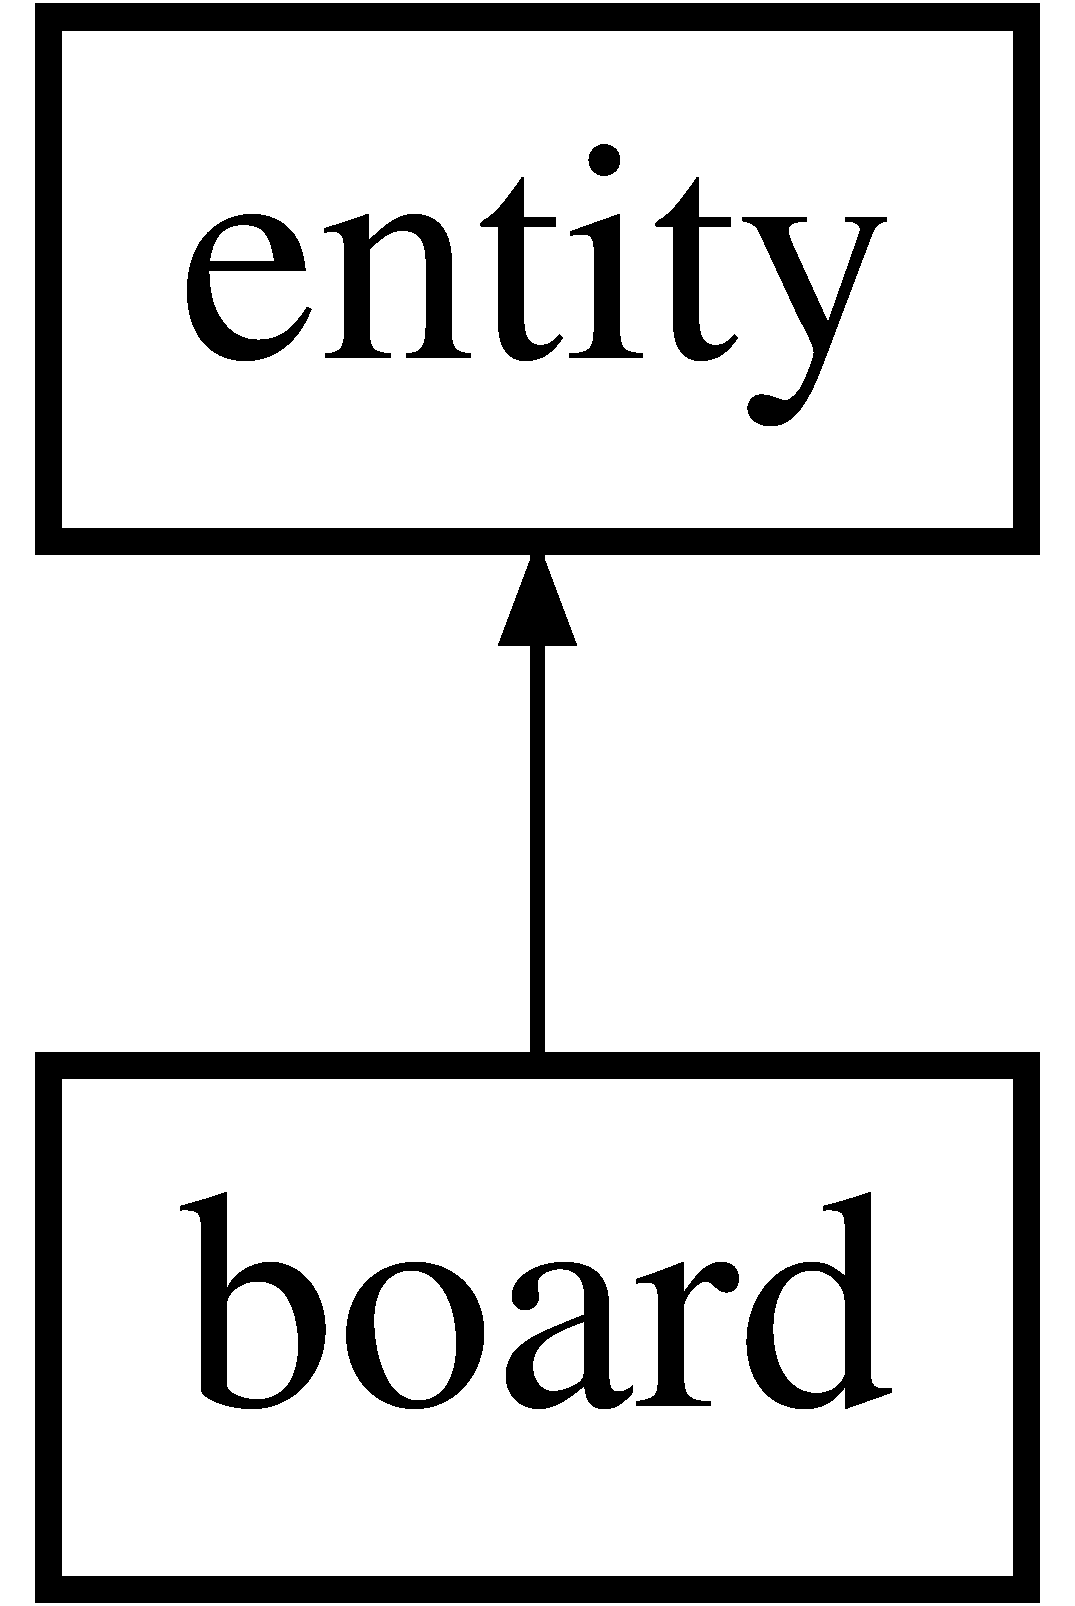
\includegraphics[height=2.000000cm]{classboard}
\end{center}
\end{figure}
\subsection*{Public Member Functions}
\begin{DoxyCompactItemize}
\item 
\mbox{\hyperlink{classboard_ae4a39ba645ad37214ecc99b4a9fe0ed1}{board}} (float x, float y, float width, float height, std\+::vector$<$ \mbox{\hyperlink{classplayer}{player}} $\ast$$>$ $\ast$players, const sf\+::\+Color board\+Color)
\item 
virtual \mbox{\hyperlink{classboard_a978427d3593354f5d735a766585a2ad2}{$\sim$board}} ()
\item 
void \mbox{\hyperlink{classboard_a092056b291f6ff6cb438903a5e416ecb}{render}} (sf\+::\+Render\+Target $\ast$target)
\item 
void \mbox{\hyperlink{classboard_a73a36842b85ae6074c10d9cd2fd8592b}{update}} (const float \&dt, sf\+::\+Vector2f mouse\+Pos)
\end{DoxyCompactItemize}
\subsection*{Additional Inherited Members}


\subsection{Detailed Description}
Klasa odpowiedzialna za plansz� do gry. Wszystkie elementy znajduj�ce si� na planszy s� tutaj inicjalizowane. 

Definition at line 5 of file board.\+h.



\subsection{Constructor \& Destructor Documentation}
\mbox{\Hypertarget{classboard_ae4a39ba645ad37214ecc99b4a9fe0ed1}\label{classboard_ae4a39ba645ad37214ecc99b4a9fe0ed1}} 
\index{board@{board}!board@{board}}
\index{board@{board}!board@{board}}
\subsubsection{\texorpdfstring{board()}{board()}}
{\footnotesize\ttfamily board\+::board (\begin{DoxyParamCaption}\item[{float}]{x,  }\item[{float}]{y,  }\item[{float}]{width,  }\item[{float}]{height,  }\item[{std\+::vector$<$ \mbox{\hyperlink{classplayer}{player}} $\ast$$>$ $\ast$}]{players,  }\item[{const sf\+::\+Color}]{board\+Color }\end{DoxyParamCaption})}

~\newline
Inicjalizuje powstanie nowej planszy. Nadaje domy�lne parametry. Inicjalizuje tekstury, zmienne, rozmiary, pozycj�, pola, graczy, tokeny, tur�, komponenty.

Definition at line 346 of file board.\+cpp.

\mbox{\Hypertarget{classboard_a978427d3593354f5d735a766585a2ad2}\label{classboard_a978427d3593354f5d735a766585a2ad2}} 
\index{board@{board}!````~board@{$\sim$board}}
\index{````~board@{$\sim$board}!board@{board}}
\subsubsection{\texorpdfstring{$\sim$board()}{~board()}}
{\footnotesize\ttfamily board\+::$\sim$board (\begin{DoxyParamCaption}{ }\end{DoxyParamCaption})\hspace{0.3cm}{\ttfamily [virtual]}}



Definition at line 365 of file board.\+cpp.



\subsection{Member Function Documentation}
\mbox{\Hypertarget{classboard_a092056b291f6ff6cb438903a5e416ecb}\label{classboard_a092056b291f6ff6cb438903a5e416ecb}} 
\index{board@{board}!render@{render}}
\index{render@{render}!board@{board}}
\subsubsection{\texorpdfstring{render()}{render()}}
{\footnotesize\ttfamily void board\+::render (\begin{DoxyParamCaption}\item[{sf\+::\+Render\+Target $\ast$}]{target }\end{DoxyParamCaption})\hspace{0.3cm}{\ttfamily [virtual]}}

~\newline
Rysuje w oknie wszystkie elementy planszy.

Reimplemented from \mbox{\hyperlink{classentity_a5b083ead5c77ab929809c662d71f37f6}{entity}}.



Definition at line 378 of file board.\+cpp.

\mbox{\Hypertarget{classboard_a73a36842b85ae6074c10d9cd2fd8592b}\label{classboard_a73a36842b85ae6074c10d9cd2fd8592b}} 
\index{board@{board}!update@{update}}
\index{update@{update}!board@{board}}
\subsubsection{\texorpdfstring{update()}{update()}}
{\footnotesize\ttfamily void board\+::update (\begin{DoxyParamCaption}\item[{const float \&}]{dt,  }\item[{sf\+::\+Vector2f}]{mouse\+Pos }\end{DoxyParamCaption})}

~\newline
Aktualizuje wszystkie elementy na planszy.

Definition at line 434 of file board.\+cpp.



The documentation for this class was generated from the following files\+:\begin{DoxyCompactItemize}
\item 
\mbox{\hyperlink{board_8h}{board.\+h}}\item 
\mbox{\hyperlink{board_8cpp}{board.\+cpp}}\end{DoxyCompactItemize}

\hypertarget{class_button}{}\section{Button Class Reference}
\label{class_button}\index{Button@{Button}}


{\ttfamily \#include $<$button.\+h$>$}

\subsection*{Public Member Functions}
\begin{DoxyCompactItemize}
\item 
\mbox{\hyperlink{class_button_a3b36df1ae23c58aedb9e15a713159459}{Button}} ()
\item 
\mbox{\hyperlink{class_button_a7219fc574a2a6d3f77d4e83edb0ec909}{Button}} (std\+::string t, sf\+::\+Vector2f size, int char\+Size, sf\+::\+Color bg\+Color, sf\+::\+Color text\+Color)
\item 
void \mbox{\hyperlink{class_button_a155eee48a55f34915319d21460ce5955}{set\+Font}} (sf\+::\+Font \&font)
\item 
void \mbox{\hyperlink{class_button_aaebeadc6fedd71472ef452302278de44}{set\+Back\+Color}} (sf\+::\+Color color)
\item 
void \mbox{\hyperlink{class_button_a0cb69f44122ef0923e6a3ea1a198257a}{set\+Text\+Color}} (sf\+::\+Color color)
\item 
void \mbox{\hyperlink{class_button_a93438906f229fb6e2ba63103140dbd9f}{set\+Position}} (sf\+::\+Vector2f pos)
\item 
void \mbox{\hyperlink{class_button_a1feaea3cde433ed7d1ef1312a3893402}{draw\+To}} (sf\+::\+Render\+Window \&window)
\item 
bool \mbox{\hyperlink{class_button_a34779d5dfdc96291a25454975c14e2b2}{is\+Mouse\+Over}} (sf\+::\+Render\+Window \&window)
\end{DoxyCompactItemize}


\subsection{Detailed Description}


Definition at line 7 of file button.\+h.



\subsection{Constructor \& Destructor Documentation}
\mbox{\Hypertarget{class_button_a3b36df1ae23c58aedb9e15a713159459}\label{class_button_a3b36df1ae23c58aedb9e15a713159459}} 
\index{Button@{Button}!Button@{Button}}
\index{Button@{Button}!Button@{Button}}
\subsubsection{\texorpdfstring{Button()}{Button()}\hspace{0.1cm}{\footnotesize\ttfamily [1/2]}}
{\footnotesize\ttfamily Button\+::\+Button (\begin{DoxyParamCaption}{ }\end{DoxyParamCaption})\hspace{0.3cm}{\ttfamily [inline]}}



Definition at line 10 of file button.\+h.

\mbox{\Hypertarget{class_button_a7219fc574a2a6d3f77d4e83edb0ec909}\label{class_button_a7219fc574a2a6d3f77d4e83edb0ec909}} 
\index{Button@{Button}!Button@{Button}}
\index{Button@{Button}!Button@{Button}}
\subsubsection{\texorpdfstring{Button()}{Button()}\hspace{0.1cm}{\footnotesize\ttfamily [2/2]}}
{\footnotesize\ttfamily Button\+::\+Button (\begin{DoxyParamCaption}\item[{std\+::string}]{t,  }\item[{sf\+::\+Vector2f}]{size,  }\item[{int}]{char\+Size,  }\item[{sf\+::\+Color}]{bg\+Color,  }\item[{sf\+::\+Color}]{text\+Color }\end{DoxyParamCaption})\hspace{0.3cm}{\ttfamily [inline]}}



Definition at line 12 of file button.\+h.



\subsection{Member Function Documentation}
\mbox{\Hypertarget{class_button_a1feaea3cde433ed7d1ef1312a3893402}\label{class_button_a1feaea3cde433ed7d1ef1312a3893402}} 
\index{Button@{Button}!draw\+To@{draw\+To}}
\index{draw\+To@{draw\+To}!Button@{Button}}
\subsubsection{\texorpdfstring{draw\+To()}{drawTo()}}
{\footnotesize\ttfamily void Button\+::draw\+To (\begin{DoxyParamCaption}\item[{sf\+::\+Render\+Window \&}]{window }\end{DoxyParamCaption})\hspace{0.3cm}{\ttfamily [inline]}}



Definition at line 44 of file button.\+h.

\mbox{\Hypertarget{class_button_a34779d5dfdc96291a25454975c14e2b2}\label{class_button_a34779d5dfdc96291a25454975c14e2b2}} 
\index{Button@{Button}!is\+Mouse\+Over@{is\+Mouse\+Over}}
\index{is\+Mouse\+Over@{is\+Mouse\+Over}!Button@{Button}}
\subsubsection{\texorpdfstring{is\+Mouse\+Over()}{isMouseOver()}}
{\footnotesize\ttfamily bool Button\+::is\+Mouse\+Over (\begin{DoxyParamCaption}\item[{sf\+::\+Render\+Window \&}]{window }\end{DoxyParamCaption})\hspace{0.3cm}{\ttfamily [inline]}}



Definition at line 50 of file button.\+h.

\mbox{\Hypertarget{class_button_aaebeadc6fedd71472ef452302278de44}\label{class_button_aaebeadc6fedd71472ef452302278de44}} 
\index{Button@{Button}!set\+Back\+Color@{set\+Back\+Color}}
\index{set\+Back\+Color@{set\+Back\+Color}!Button@{Button}}
\subsubsection{\texorpdfstring{set\+Back\+Color()}{setBackColor()}}
{\footnotesize\ttfamily void Button\+::set\+Back\+Color (\begin{DoxyParamCaption}\item[{sf\+::\+Color}]{color }\end{DoxyParamCaption})\hspace{0.3cm}{\ttfamily [inline]}}



Definition at line 26 of file button.\+h.

\mbox{\Hypertarget{class_button_a155eee48a55f34915319d21460ce5955}\label{class_button_a155eee48a55f34915319d21460ce5955}} 
\index{Button@{Button}!set\+Font@{set\+Font}}
\index{set\+Font@{set\+Font}!Button@{Button}}
\subsubsection{\texorpdfstring{set\+Font()}{setFont()}}
{\footnotesize\ttfamily void Button\+::set\+Font (\begin{DoxyParamCaption}\item[{sf\+::\+Font \&}]{font }\end{DoxyParamCaption})\hspace{0.3cm}{\ttfamily [inline]}}



Definition at line 22 of file button.\+h.

\mbox{\Hypertarget{class_button_a93438906f229fb6e2ba63103140dbd9f}\label{class_button_a93438906f229fb6e2ba63103140dbd9f}} 
\index{Button@{Button}!set\+Position@{set\+Position}}
\index{set\+Position@{set\+Position}!Button@{Button}}
\subsubsection{\texorpdfstring{set\+Position()}{setPosition()}}
{\footnotesize\ttfamily void Button\+::set\+Position (\begin{DoxyParamCaption}\item[{sf\+::\+Vector2f}]{pos }\end{DoxyParamCaption})\hspace{0.3cm}{\ttfamily [inline]}}



Definition at line 33 of file button.\+h.

\mbox{\Hypertarget{class_button_a0cb69f44122ef0923e6a3ea1a198257a}\label{class_button_a0cb69f44122ef0923e6a3ea1a198257a}} 
\index{Button@{Button}!set\+Text\+Color@{set\+Text\+Color}}
\index{set\+Text\+Color@{set\+Text\+Color}!Button@{Button}}
\subsubsection{\texorpdfstring{set\+Text\+Color()}{setTextColor()}}
{\footnotesize\ttfamily void Button\+::set\+Text\+Color (\begin{DoxyParamCaption}\item[{sf\+::\+Color}]{color }\end{DoxyParamCaption})\hspace{0.3cm}{\ttfamily [inline]}}



Definition at line 30 of file button.\+h.



The documentation for this class was generated from the following file\+:\begin{DoxyCompactItemize}
\item 
from\+\_\+previous\+\_\+tuts/\mbox{\hyperlink{button_8h}{button.\+h}}\end{DoxyCompactItemize}

\hypertarget{classgui_1_1button}{}\section{gui\+:\+:button Class Reference}
\label{classgui_1_1button}\index{gui\+::button@{gui\+::button}}


{\ttfamily \#include $<$gui.\+h$>$}

\subsection*{Public Member Functions}
\begin{DoxyCompactItemize}
\item 
\mbox{\hyperlink{classgui_1_1button_ae0f718c924c548b17aa3637e22b3de27}{button}} (float x, float y, float width, float height, sf\+::\+Font $\ast$font, std\+::string \mbox{\hyperlink{classgui_1_1button_a5f95923cae850d453ebed23eb759e84a}{text}}, sf\+::\+Color idle\+Color, sf\+::\+Color hover\+Color, sf\+::\+Color pressed\+Color)
\item 
virtual \mbox{\hyperlink{classgui_1_1button_aff168bb8fb7c36888cbccb3750558f65}{$\sim$button}} ()
\item 
const bool \mbox{\hyperlink{classgui_1_1button_aa03c22e8dd1ce6cfbddc71bf0365831e}{is\+Pressed}} () const
\item 
void \mbox{\hyperlink{classgui_1_1button_a28031233c189ce7fa86b1f2a2cb81413}{block\+Button}} ()
\item 
void \mbox{\hyperlink{classgui_1_1button_af804e1dbdf79c46f2d23e6dc05e3b827}{unblock\+Button}} ()
\item 
const bool \mbox{\hyperlink{classgui_1_1button_aeae7443bf73898b5fa193a82f66c1934}{get\+Key\+Time}} ()
\item 
void \mbox{\hyperlink{classgui_1_1button_add8e160f9649b1acf409185fc8569f5a}{update\+Key\+Time}} (const float \&dt)
\item 
void \mbox{\hyperlink{classgui_1_1button_a931a0a0d5f9e3a1d60281ea37287ec90}{update}} (sf\+::\+Vector2f mouse\+Pos, const float \&dt)
\item 
void \mbox{\hyperlink{classgui_1_1button_afc80af563256b7f63c6e85e5017d9bdd}{render}} (sf\+::\+Render\+Target $\ast$target)
\end{DoxyCompactItemize}
\subsection*{Public Attributes}
\begin{DoxyCompactItemize}
\item 
sf\+::\+Text \mbox{\hyperlink{classgui_1_1button_a5f95923cae850d453ebed23eb759e84a}{text}}
\end{DoxyCompactItemize}


\subsection{Detailed Description}
Klasa przycisku. Od�wie�any z zadan� cz�stotliwo�ci�. 

Definition at line 27 of file gui.\+h.



\subsection{Constructor \& Destructor Documentation}
\mbox{\Hypertarget{classgui_1_1button_ae0f718c924c548b17aa3637e22b3de27}\label{classgui_1_1button_ae0f718c924c548b17aa3637e22b3de27}} 
\index{gui\+::button@{gui\+::button}!button@{button}}
\index{button@{button}!gui\+::button@{gui\+::button}}
\subsubsection{\texorpdfstring{button()}{button()}}
{\footnotesize\ttfamily gui\+::button\+::button (\begin{DoxyParamCaption}\item[{float}]{x,  }\item[{float}]{y,  }\item[{float}]{width,  }\item[{float}]{height,  }\item[{sf\+::\+Font $\ast$}]{font,  }\item[{std\+::string}]{text,  }\item[{sf\+::\+Color}]{idle\+Color,  }\item[{sf\+::\+Color}]{hover\+Color,  }\item[{sf\+::\+Color}]{pressed\+Color }\end{DoxyParamCaption})}

~\newline
Tworzy przycisk z zadanych parametr�w. Domy�lnie nie jest zablokowany.

Definition at line 4 of file gui.\+cpp.

\mbox{\Hypertarget{classgui_1_1button_aff168bb8fb7c36888cbccb3750558f65}\label{classgui_1_1button_aff168bb8fb7c36888cbccb3750558f65}} 
\index{gui\+::button@{gui\+::button}!````~button@{$\sim$button}}
\index{````~button@{$\sim$button}!gui\+::button@{gui\+::button}}
\subsubsection{\texorpdfstring{$\sim$button()}{~button()}}
{\footnotesize\ttfamily gui\+::button\+::$\sim$button (\begin{DoxyParamCaption}{ }\end{DoxyParamCaption})\hspace{0.3cm}{\ttfamily [virtual]}}



Definition at line 59 of file gui.\+cpp.



\subsection{Member Function Documentation}
\mbox{\Hypertarget{classgui_1_1button_a28031233c189ce7fa86b1f2a2cb81413}\label{classgui_1_1button_a28031233c189ce7fa86b1f2a2cb81413}} 
\index{gui\+::button@{gui\+::button}!block\+Button@{block\+Button}}
\index{block\+Button@{block\+Button}!gui\+::button@{gui\+::button}}
\subsubsection{\texorpdfstring{block\+Button()}{blockButton()}}
{\footnotesize\ttfamily void gui\+::button\+::block\+Button (\begin{DoxyParamCaption}{ }\end{DoxyParamCaption})}

~\newline
Blokuje przycisk, zmieniaj�c flag� blocked na true

Definition at line 77 of file gui.\+cpp.

\mbox{\Hypertarget{classgui_1_1button_aeae7443bf73898b5fa193a82f66c1934}\label{classgui_1_1button_aeae7443bf73898b5fa193a82f66c1934}} 
\index{gui\+::button@{gui\+::button}!get\+Key\+Time@{get\+Key\+Time}}
\index{get\+Key\+Time@{get\+Key\+Time}!gui\+::button@{gui\+::button}}
\subsubsection{\texorpdfstring{get\+Key\+Time()}{getKeyTime()}}
{\footnotesize\ttfamily const bool gui\+::button\+::get\+Key\+Time (\begin{DoxyParamCaption}{ }\end{DoxyParamCaption})}

~\newline
Pobiera aktualny czas przycisku.

Definition at line 94 of file gui.\+cpp.

\mbox{\Hypertarget{classgui_1_1button_aa03c22e8dd1ce6cfbddc71bf0365831e}\label{classgui_1_1button_aa03c22e8dd1ce6cfbddc71bf0365831e}} 
\index{gui\+::button@{gui\+::button}!is\+Pressed@{is\+Pressed}}
\index{is\+Pressed@{is\+Pressed}!gui\+::button@{gui\+::button}}
\subsubsection{\texorpdfstring{is\+Pressed()}{isPressed()}}
{\footnotesize\ttfamily const bool gui\+::button\+::is\+Pressed (\begin{DoxyParamCaption}{ }\end{DoxyParamCaption}) const}

~\newline
Sprawdza stan wci�ni�cia przycisku.

Definition at line 67 of file gui.\+cpp.

\mbox{\Hypertarget{classgui_1_1button_afc80af563256b7f63c6e85e5017d9bdd}\label{classgui_1_1button_afc80af563256b7f63c6e85e5017d9bdd}} 
\index{gui\+::button@{gui\+::button}!render@{render}}
\index{render@{render}!gui\+::button@{gui\+::button}}
\subsubsection{\texorpdfstring{render()}{render()}}
{\footnotesize\ttfamily void gui\+::button\+::render (\begin{DoxyParamCaption}\item[{sf\+::\+Render\+Target $\ast$}]{target }\end{DoxyParamCaption})}



Definition at line 168 of file gui.\+cpp.

\mbox{\Hypertarget{classgui_1_1button_af804e1dbdf79c46f2d23e6dc05e3b827}\label{classgui_1_1button_af804e1dbdf79c46f2d23e6dc05e3b827}} 
\index{gui\+::button@{gui\+::button}!unblock\+Button@{unblock\+Button}}
\index{unblock\+Button@{unblock\+Button}!gui\+::button@{gui\+::button}}
\subsubsection{\texorpdfstring{unblock\+Button()}{unblockButton()}}
{\footnotesize\ttfamily void gui\+::button\+::unblock\+Button (\begin{DoxyParamCaption}{ }\end{DoxyParamCaption})}

~\newline
I\+Odblokowuje przycisk poprzez zmian� flagi blocked na false.

Definition at line 85 of file gui.\+cpp.

\mbox{\Hypertarget{classgui_1_1button_a931a0a0d5f9e3a1d60281ea37287ec90}\label{classgui_1_1button_a931a0a0d5f9e3a1d60281ea37287ec90}} 
\index{gui\+::button@{gui\+::button}!update@{update}}
\index{update@{update}!gui\+::button@{gui\+::button}}
\subsubsection{\texorpdfstring{update()}{update()}}
{\footnotesize\ttfamily void gui\+::button\+::update (\begin{DoxyParamCaption}\item[{sf\+::\+Vector2f}]{mouse\+Pos,  }\item[{const float \&}]{dt }\end{DoxyParamCaption})}

~\newline
I\+Aktualizuje stan przycisku. Sprawdza, czy kursor jest nad przyciskiem, czy jest wci�ni�ty, zablokowany.

Definition at line 122 of file gui.\+cpp.

\mbox{\Hypertarget{classgui_1_1button_add8e160f9649b1acf409185fc8569f5a}\label{classgui_1_1button_add8e160f9649b1acf409185fc8569f5a}} 
\index{gui\+::button@{gui\+::button}!update\+Key\+Time@{update\+Key\+Time}}
\index{update\+Key\+Time@{update\+Key\+Time}!gui\+::button@{gui\+::button}}
\subsubsection{\texorpdfstring{update\+Key\+Time()}{updateKeyTime()}}
{\footnotesize\ttfamily void gui\+::button\+::update\+Key\+Time (\begin{DoxyParamCaption}\item[{const float \&}]{dt }\end{DoxyParamCaption})}

~\newline
Aktualizuje czas przycisku. Pozwala na unikni�cie wielokliku przy d�u�szym przytrzymaniu myszy.

Definition at line 109 of file gui.\+cpp.



\subsection{Member Data Documentation}
\mbox{\Hypertarget{classgui_1_1button_a5f95923cae850d453ebed23eb759e84a}\label{classgui_1_1button_a5f95923cae850d453ebed23eb759e84a}} 
\index{gui\+::button@{gui\+::button}!text@{text}}
\index{text@{text}!gui\+::button@{gui\+::button}}
\subsubsection{\texorpdfstring{text}{text}}
{\footnotesize\ttfamily sf\+::\+Text gui\+::button\+::text}



Definition at line 47 of file gui.\+h.



The documentation for this class was generated from the following files\+:\begin{DoxyCompactItemize}
\item 
\mbox{\hyperlink{gui_8h}{gui.\+h}}\item 
\mbox{\hyperlink{gui_8cpp}{gui.\+cpp}}\end{DoxyCompactItemize}

\hypertarget{classentity}{}\section{entity Class Reference}
\label{classentity}\index{entity@{entity}}


{\ttfamily \#include $<$entity.\+h$>$}

Inheritance diagram for entity\+:\begin{figure}[H]
\begin{center}
\leavevmode
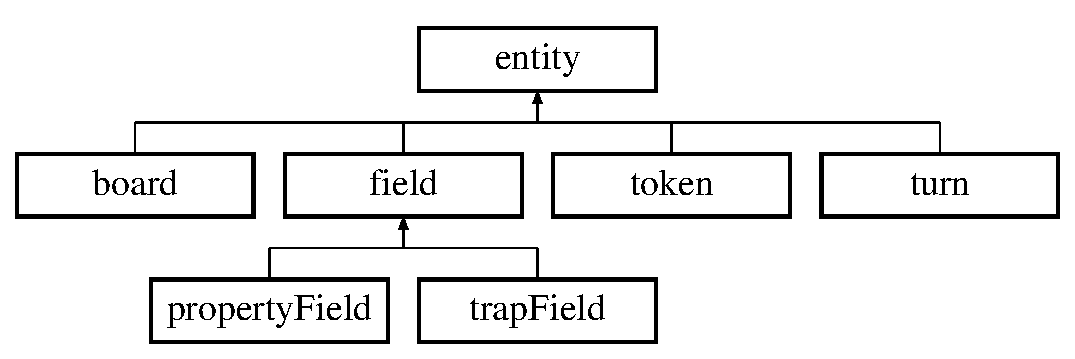
\includegraphics[height=3.000000cm]{classentity}
\end{center}
\end{figure}
\subsection*{Public Member Functions}
\begin{DoxyCompactItemize}
\item 
\mbox{\hyperlink{classentity_ac20edb72e9e89b902bf14b68773c1697}{entity}} ()
\item 
virtual \mbox{\hyperlink{classentity_acec2b315e0eddb40f6c2dc1a7688293e}{$\sim$entity}} ()
\item 
void \mbox{\hyperlink{classentity_ae1b6f11cf4d1a47d9c41d45c33ee24c1}{create\+Sprite}} (sf\+::\+Texture $\ast$\mbox{\hyperlink{classentity_aeb2014309ee421c4185f64f8cb6f6b30}{texture}})
\item 
void \mbox{\hyperlink{classentity_ad9b68be56e131ee899fa246ea542f96f}{create\+Rect}} (float width, float height, sf\+::\+Color color, bool origin\+In\+Center)
\item 
void \mbox{\hyperlink{classentity_ab3d4b23d67cad72fe9b8192666b188be}{set\+Origin\+In\+Center}} ()
\item 
virtual void \mbox{\hyperlink{classentity_a1ff6bad3b872130413e664fa14965b1b}{set\+Position}} (const float x, const float y)
\item 
virtual void \mbox{\hyperlink{classentity_a9fb61b5564720c7e61d55c312b0448c8}{move}} (const float \&dt, const float dir\+\_\+x, const float dir\+\_\+y)
\item 
virtual void \mbox{\hyperlink{classentity_a155484fa64039b2e359cc2a99a6f09f5}{update}} (const float \&dt)
\item 
virtual void \mbox{\hyperlink{classentity_a5b083ead5c77ab929809c662d71f37f6}{render}} (sf\+::\+Render\+Target $\ast$target)
\end{DoxyCompactItemize}
\subsection*{Public Attributes}
\begin{DoxyCompactItemize}
\item 
sf\+::\+Sprite $\ast$ \mbox{\hyperlink{classentity_a14af3c2af6f81ed514bf0398579049ba}{sprite}}
\end{DoxyCompactItemize}
\subsection*{Protected Member Functions}
\begin{DoxyCompactItemize}
\item 
virtual void \mbox{\hyperlink{classentity_a35315b580fda3763cfeb87b6dec77879}{scale\+Fonts}} ()
\end{DoxyCompactItemize}
\subsection*{Protected Attributes}
\begin{DoxyCompactItemize}
\item 
sf\+::\+Texture $\ast$ \mbox{\hyperlink{classentity_aeb2014309ee421c4185f64f8cb6f6b30}{texture}}
\item 
sf\+::\+Font \mbox{\hyperlink{classentity_ace4c257849221c29427f2abfbcb35074}{font}}
\item 
sf\+::\+Rectangle\+Shape $\ast$ \mbox{\hyperlink{classentity_af5e82b825396fabe621e707ca670b011}{default\+Shape}}
\item 
std\+::map$<$ unsigned short, int $>$ \mbox{\hyperlink{classentity_a2b2741d5d3818e5d6d8c583dc92d2a14}{font\+Size}}
\item 
bool \mbox{\hyperlink{classentity_ab82c76511fa953eb60ba08419317bbaa}{load\+Texture}}
\item 
float \mbox{\hyperlink{classentity_a446075bd01281cbb7be7ec8bf69fc2e2}{movement\+Speed}}
\end{DoxyCompactItemize}


\subsection{Detailed Description}
Klasa abstrakcyjna okre�laj�ca ka�dy element znajduj�cy si� na planszy, maj�cy graficzne przedstawienie. 

Definition at line 20 of file entity.\+h.



\subsection{Constructor \& Destructor Documentation}
\mbox{\Hypertarget{classentity_ac20edb72e9e89b902bf14b68773c1697}\label{classentity_ac20edb72e9e89b902bf14b68773c1697}} 
\index{entity@{entity}!entity@{entity}}
\index{entity@{entity}!entity@{entity}}
\subsubsection{\texorpdfstring{entity()}{entity()}}
{\footnotesize\ttfamily entity\+::entity (\begin{DoxyParamCaption}{ }\end{DoxyParamCaption})}



Definition at line 37 of file entity.\+cpp.

\mbox{\Hypertarget{classentity_acec2b315e0eddb40f6c2dc1a7688293e}\label{classentity_acec2b315e0eddb40f6c2dc1a7688293e}} 
\index{entity@{entity}!````~entity@{$\sim$entity}}
\index{````~entity@{$\sim$entity}!entity@{entity}}
\subsubsection{\texorpdfstring{$\sim$entity()}{~entity()}}
{\footnotesize\ttfamily entity\+::$\sim$entity (\begin{DoxyParamCaption}{ }\end{DoxyParamCaption})\hspace{0.3cm}{\ttfamily [virtual]}}



Definition at line 42 of file entity.\+cpp.



\subsection{Member Function Documentation}
\mbox{\Hypertarget{classentity_ad9b68be56e131ee899fa246ea542f96f}\label{classentity_ad9b68be56e131ee899fa246ea542f96f}} 
\index{entity@{entity}!create\+Rect@{create\+Rect}}
\index{create\+Rect@{create\+Rect}!entity@{entity}}
\subsubsection{\texorpdfstring{create\+Rect()}{createRect()}}
{\footnotesize\ttfamily void entity\+::create\+Rect (\begin{DoxyParamCaption}\item[{float}]{width,  }\item[{float}]{height,  }\item[{sf\+::\+Color}]{color,  }\item[{bool}]{origin\+In\+Center }\end{DoxyParamCaption})}

~\newline
Tworzy prostok�t, maj�c dane parametry. Pozwala na umieszczenie uchwytu w �rodku za pomoc� origin\+In\+Center.

Definition at line 62 of file entity.\+cpp.

\mbox{\Hypertarget{classentity_ae1b6f11cf4d1a47d9c41d45c33ee24c1}\label{classentity_ae1b6f11cf4d1a47d9c41d45c33ee24c1}} 
\index{entity@{entity}!create\+Sprite@{create\+Sprite}}
\index{create\+Sprite@{create\+Sprite}!entity@{entity}}
\subsubsection{\texorpdfstring{create\+Sprite()}{createSprite()}}
{\footnotesize\ttfamily void entity\+::create\+Sprite (\begin{DoxyParamCaption}\item[{sf\+::\+Texture $\ast$}]{texture }\end{DoxyParamCaption})}

~\newline
Pozwala na u�ycie tekstury.

Definition at line 51 of file entity.\+cpp.

\mbox{\Hypertarget{classentity_a9fb61b5564720c7e61d55c312b0448c8}\label{classentity_a9fb61b5564720c7e61d55c312b0448c8}} 
\index{entity@{entity}!move@{move}}
\index{move@{move}!entity@{entity}}
\subsubsection{\texorpdfstring{move()}{move()}}
{\footnotesize\ttfamily void entity\+::move (\begin{DoxyParamCaption}\item[{const float \&}]{dt,  }\item[{const float}]{dir\+\_\+x,  }\item[{const float}]{dir\+\_\+y }\end{DoxyParamCaption})\hspace{0.3cm}{\ttfamily [virtual]}}

~\newline
I\+Pozwala na poruszenie obiektu z zadan� pr�dko�ci�.

Definition at line 111 of file entity.\+cpp.

\mbox{\Hypertarget{classentity_a5b083ead5c77ab929809c662d71f37f6}\label{classentity_a5b083ead5c77ab929809c662d71f37f6}} 
\index{entity@{entity}!render@{render}}
\index{render@{render}!entity@{entity}}
\subsubsection{\texorpdfstring{render()}{render()}}
{\footnotesize\ttfamily void entity\+::render (\begin{DoxyParamCaption}\item[{sf\+::\+Render\+Target $\ast$}]{target }\end{DoxyParamCaption})\hspace{0.3cm}{\ttfamily [virtual]}}

~\newline
Rysuje entity. Je�li dodana zosta�a tekstura to rysuje tekstur�, w przeciwnym razie rysuje default\+Shape, czyli domy�lny kszta�t b�d�cy prostok�tem.

Reimplemented in \mbox{\hyperlink{classproperty_field_ada6c23589e09fe31f88b75ed2ec27d11}{property\+Field}}, \mbox{\hyperlink{classboard_a092056b291f6ff6cb438903a5e416ecb}{board}}, \mbox{\hyperlink{classturn_a6a72d11a8e3d8272c6b8d1ddd66331c2}{turn}}, and \mbox{\hyperlink{classfield_a3b2cdb0e289aa1b47ce79360b975f6a9}{field}}.



Definition at line 128 of file entity.\+cpp.

\mbox{\Hypertarget{classentity_a35315b580fda3763cfeb87b6dec77879}\label{classentity_a35315b580fda3763cfeb87b6dec77879}} 
\index{entity@{entity}!scale\+Fonts@{scale\+Fonts}}
\index{scale\+Fonts@{scale\+Fonts}!entity@{entity}}
\subsubsection{\texorpdfstring{scale\+Fonts()}{scaleFonts()}}
{\footnotesize\ttfamily void entity\+::scale\+Fonts (\begin{DoxyParamCaption}{ }\end{DoxyParamCaption})\hspace{0.3cm}{\ttfamily [protected]}, {\ttfamily [virtual]}}

~\newline
Skaluje czcionk� w zale�no�ci od wielko�ci elementu.

Definition at line 23 of file entity.\+cpp.

\mbox{\Hypertarget{classentity_ab3d4b23d67cad72fe9b8192666b188be}\label{classentity_ab3d4b23d67cad72fe9b8192666b188be}} 
\index{entity@{entity}!set\+Origin\+In\+Center@{set\+Origin\+In\+Center}}
\index{set\+Origin\+In\+Center@{set\+Origin\+In\+Center}!entity@{entity}}
\subsubsection{\texorpdfstring{set\+Origin\+In\+Center()}{setOriginInCenter()}}
{\footnotesize\ttfamily void entity\+::set\+Origin\+In\+Center (\begin{DoxyParamCaption}{ }\end{DoxyParamCaption})}

~\newline
Umieszcza uchwyt obiektu w �rodku ci�ko�ci.

Definition at line 98 of file entity.\+cpp.

\mbox{\Hypertarget{classentity_a1ff6bad3b872130413e664fa14965b1b}\label{classentity_a1ff6bad3b872130413e664fa14965b1b}} 
\index{entity@{entity}!set\+Position@{set\+Position}}
\index{set\+Position@{set\+Position}!entity@{entity}}
\subsubsection{\texorpdfstring{set\+Position()}{setPosition()}}
{\footnotesize\ttfamily void entity\+::set\+Position (\begin{DoxyParamCaption}\item[{const float}]{x,  }\item[{const float}]{y }\end{DoxyParamCaption})\hspace{0.3cm}{\ttfamily [virtual]}}

~\newline
Ustawia pozycj� elementu.

Definition at line 80 of file entity.\+cpp.

\mbox{\Hypertarget{classentity_a155484fa64039b2e359cc2a99a6f09f5}\label{classentity_a155484fa64039b2e359cc2a99a6f09f5}} 
\index{entity@{entity}!update@{update}}
\index{update@{update}!entity@{entity}}
\subsubsection{\texorpdfstring{update()}{update()}}
{\footnotesize\ttfamily void entity\+::update (\begin{DoxyParamCaption}\item[{const float \&}]{dt }\end{DoxyParamCaption})\hspace{0.3cm}{\ttfamily [virtual]}}



Reimplemented in \mbox{\hyperlink{classtoken_aafed3b67f7f8466510d6bd4e93413e15}{token}}.



Definition at line 123 of file entity.\+cpp.



\subsection{Member Data Documentation}
\mbox{\Hypertarget{classentity_af5e82b825396fabe621e707ca670b011}\label{classentity_af5e82b825396fabe621e707ca670b011}} 
\index{entity@{entity}!default\+Shape@{default\+Shape}}
\index{default\+Shape@{default\+Shape}!entity@{entity}}
\subsubsection{\texorpdfstring{default\+Shape}{defaultShape}}
{\footnotesize\ttfamily sf\+::\+Rectangle\+Shape$\ast$ entity\+::default\+Shape\hspace{0.3cm}{\ttfamily [protected]}}



Definition at line 40 of file entity.\+h.

\mbox{\Hypertarget{classentity_ace4c257849221c29427f2abfbcb35074}\label{classentity_ace4c257849221c29427f2abfbcb35074}} 
\index{entity@{entity}!font@{font}}
\index{font@{font}!entity@{entity}}
\subsubsection{\texorpdfstring{font}{font}}
{\footnotesize\ttfamily sf\+::\+Font entity\+::font\hspace{0.3cm}{\ttfamily [protected]}}



Definition at line 39 of file entity.\+h.

\mbox{\Hypertarget{classentity_a2b2741d5d3818e5d6d8c583dc92d2a14}\label{classentity_a2b2741d5d3818e5d6d8c583dc92d2a14}} 
\index{entity@{entity}!font\+Size@{font\+Size}}
\index{font\+Size@{font\+Size}!entity@{entity}}
\subsubsection{\texorpdfstring{font\+Size}{fontSize}}
{\footnotesize\ttfamily std\+::map$<$unsigned short, int$>$ entity\+::font\+Size\hspace{0.3cm}{\ttfamily [protected]}}



Definition at line 41 of file entity.\+h.

\mbox{\Hypertarget{classentity_ab82c76511fa953eb60ba08419317bbaa}\label{classentity_ab82c76511fa953eb60ba08419317bbaa}} 
\index{entity@{entity}!load\+Texture@{load\+Texture}}
\index{load\+Texture@{load\+Texture}!entity@{entity}}
\subsubsection{\texorpdfstring{load\+Texture}{loadTexture}}
{\footnotesize\ttfamily bool entity\+::load\+Texture\hspace{0.3cm}{\ttfamily [protected]}}



Definition at line 42 of file entity.\+h.

\mbox{\Hypertarget{classentity_a446075bd01281cbb7be7ec8bf69fc2e2}\label{classentity_a446075bd01281cbb7be7ec8bf69fc2e2}} 
\index{entity@{entity}!movement\+Speed@{movement\+Speed}}
\index{movement\+Speed@{movement\+Speed}!entity@{entity}}
\subsubsection{\texorpdfstring{movement\+Speed}{movementSpeed}}
{\footnotesize\ttfamily float entity\+::movement\+Speed\hspace{0.3cm}{\ttfamily [protected]}}



Definition at line 46 of file entity.\+h.

\mbox{\Hypertarget{classentity_a14af3c2af6f81ed514bf0398579049ba}\label{classentity_a14af3c2af6f81ed514bf0398579049ba}} 
\index{entity@{entity}!sprite@{sprite}}
\index{sprite@{sprite}!entity@{entity}}
\subsubsection{\texorpdfstring{sprite}{sprite}}
{\footnotesize\ttfamily sf\+::\+Sprite$\ast$ entity\+::sprite}



Definition at line 51 of file entity.\+h.

\mbox{\Hypertarget{classentity_aeb2014309ee421c4185f64f8cb6f6b30}\label{classentity_aeb2014309ee421c4185f64f8cb6f6b30}} 
\index{entity@{entity}!texture@{texture}}
\index{texture@{texture}!entity@{entity}}
\subsubsection{\texorpdfstring{texture}{texture}}
{\footnotesize\ttfamily sf\+::\+Texture$\ast$ entity\+::texture\hspace{0.3cm}{\ttfamily [protected]}}



Definition at line 38 of file entity.\+h.



The documentation for this class was generated from the following files\+:\begin{DoxyCompactItemize}
\item 
\mbox{\hyperlink{entity_8h}{entity.\+h}}\item 
\mbox{\hyperlink{entity_8cpp}{entity.\+cpp}}\end{DoxyCompactItemize}

\hypertarget{classfield}{}\section{field Class Reference}
\label{classfield}\index{field@{field}}


{\ttfamily \#include $<$field.\+h$>$}

Inheritance diagram for field\+:\begin{figure}[H]
\begin{center}
\leavevmode
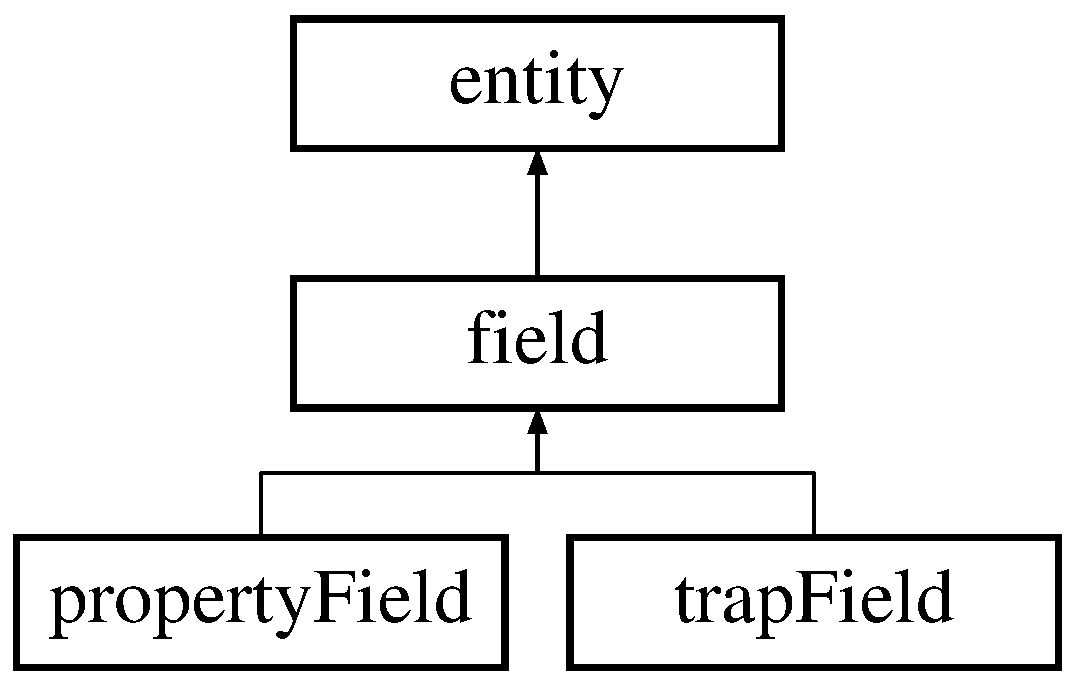
\includegraphics[height=3.000000cm]{classfield}
\end{center}
\end{figure}
\subsection*{Public Member Functions}
\begin{DoxyCompactItemize}
\item 
\mbox{\hyperlink{classfield_a35665d2e0c29e9125ae8ad082600254a}{field}} ()
\item 
virtual \mbox{\hyperlink{classfield_a600cf76c8c366764a8e0e6a48e43d0fd}{$\sim$field}} ()
\item 
virtual void \mbox{\hyperlink{classfield_a4a30d7fe2bdc0084b4b9a5f102c31e39}{init\+Token\+Slots}} ()
\item 
virtual void \mbox{\hyperlink{classfield_a940f9ab5e5a33ce71f77c88c5b312300}{on\+Step\+Action}} (\mbox{\hyperlink{classplayer}{player}} $\ast$\mbox{\hyperlink{classfield_a52e61f57f292aadd141aecf8745b4605}{player\+On\+Field}})=0
\item 
virtual void \mbox{\hyperlink{classfield_a3b2cdb0e289aa1b47ce79360b975f6a9}{render}} (sf\+::\+Render\+Target $\ast$target)
\item 
virtual void \mbox{\hyperlink{classfield_a526cc088056de1c0efdcf55fe1062e78}{update}} (const float \&dt, sf\+::\+Vector2f mouse\+Pos)
\item 
virtual sf\+::\+Vector2f \mbox{\hyperlink{classfield_a7346dd19ca40aff0739451ed99cda6cb}{get\+Token\+Slot}} ()
\end{DoxyCompactItemize}
\subsection*{Public Attributes}
\begin{DoxyCompactItemize}
\item 
unsigned int \mbox{\hyperlink{classfield_ac829935acd985295259828967292eb91}{ID}}
\item 
std\+::map$<$ int, sf\+::\+Vector2f $>$ \mbox{\hyperlink{classfield_a728e63bc476730a19d24e0b9e51da371}{token\+Slots}}
\item 
sf\+::\+Text \mbox{\hyperlink{classfield_ab03c33568f190a5c3ca4d33b4cd778ba}{field\+Type}}
\item 
sf\+::\+Text \mbox{\hyperlink{classfield_aa1ee6124b7b2c31a8cf5b72b2a1e378e}{field\+Description}}
\end{DoxyCompactItemize}
\subsection*{Protected Member Functions}
\begin{DoxyCompactItemize}
\item 
virtual void \mbox{\hyperlink{classfield_a4f68652f2eecabec8db421ac426e77b5}{create\+And\+Set\+Title\+Bar}} ()
\item 
virtual void \mbox{\hyperlink{classfield_a9341d5cedf072190186199f9abea728f}{set\+Field\+Text}} (sf\+::\+Text $\ast$field\+Text, float x, float y, int rotation, sf\+::\+Font \mbox{\hyperlink{classfield_a1aff76778baa8007044831e512a5cd8e}{font}}, int \mbox{\hyperlink{classentity_a2b2741d5d3818e5d6d8c583dc92d2a14}{font\+Size}}, sf\+::\+Color \mbox{\hyperlink{classfield_ae869b5c6466855de5bb00a0da4a738e4}{color}}, std\+::string text)
\item 
virtual void \mbox{\hyperlink{classfield_a9f906f786bd394d927f37f5004bfdcb9}{charge\+Player}} (\mbox{\hyperlink{classplayer}{player}} $\ast$\mbox{\hyperlink{classfield_a52e61f57f292aadd141aecf8745b4605}{player\+On\+Field}}, int sum)
\end{DoxyCompactItemize}
\subsection*{Protected Attributes}
\begin{DoxyCompactItemize}
\item 
sf\+::\+Text $\ast$ \mbox{\hyperlink{classfield_a0fa76e9bb3e439757ad10e5f6032e1ff}{field\+Title}}
\item 
sf\+::\+Font \mbox{\hyperlink{classfield_a1aff76778baa8007044831e512a5cd8e}{font}}
\item 
sf\+::\+Color \mbox{\hyperlink{classfield_ae869b5c6466855de5bb00a0da4a738e4}{color}}
\item 
sf\+::\+Rectangle\+Shape $\ast$ \mbox{\hyperlink{classfield_a457df0c383be6b883d441c4501d5b985}{title\+Bar}}
\item 
\mbox{\hyperlink{classplayer}{player}} $\ast$ \mbox{\hyperlink{classfield_a52e61f57f292aadd141aecf8745b4605}{player\+On\+Field}}
\item 
int \mbox{\hyperlink{classfield_ad87fbe2da895412c846878e41e673650}{cnt}}
\end{DoxyCompactItemize}


\subsection{Detailed Description}
Klasa abstrakcyjna p�l na planszy. Ka�de pole ma unikaln� definicj� czysto wirtualnej metody \mbox{\hyperlink{classfield_a940f9ab5e5a33ce71f77c88c5b312300}{on\+Step\+Action()}}. 

Definition at line 6 of file field.\+h.



\subsection{Constructor \& Destructor Documentation}
\mbox{\Hypertarget{classfield_a35665d2e0c29e9125ae8ad082600254a}\label{classfield_a35665d2e0c29e9125ae8ad082600254a}} 
\index{field@{field}!field@{field}}
\index{field@{field}!field@{field}}
\subsubsection{\texorpdfstring{field()}{field()}}
{\footnotesize\ttfamily field\+::field (\begin{DoxyParamCaption}{ }\end{DoxyParamCaption})}

~\newline
Tworzy nowy obiekt pola z czcionk� z lokalizacji /fonts. Skaluje czcionk� odpowiedni do rozmiaru planszy. Domy�lnie nie dopuszcza mo�liwo�ci tekstury.

Definition at line 6 of file field.\+cpp.

\mbox{\Hypertarget{classfield_a600cf76c8c366764a8e0e6a48e43d0fd}\label{classfield_a600cf76c8c366764a8e0e6a48e43d0fd}} 
\index{field@{field}!````~field@{$\sim$field}}
\index{````~field@{$\sim$field}!field@{field}}
\subsubsection{\texorpdfstring{$\sim$field()}{~field()}}
{\footnotesize\ttfamily field\+::$\sim$field (\begin{DoxyParamCaption}{ }\end{DoxyParamCaption})\hspace{0.3cm}{\ttfamily [virtual]}}



Definition at line 23 of file field.\+cpp.



\subsection{Member Function Documentation}
\mbox{\Hypertarget{classfield_a9f906f786bd394d927f37f5004bfdcb9}\label{classfield_a9f906f786bd394d927f37f5004bfdcb9}} 
\index{field@{field}!charge\+Player@{charge\+Player}}
\index{charge\+Player@{charge\+Player}!field@{field}}
\subsubsection{\texorpdfstring{charge\+Player()}{chargePlayer()}}
{\footnotesize\ttfamily void field\+::charge\+Player (\begin{DoxyParamCaption}\item[{\mbox{\hyperlink{classplayer}{player}} $\ast$}]{player\+On\+Field,  }\item[{int}]{sum }\end{DoxyParamCaption})\hspace{0.3cm}{\ttfamily [protected]}, {\ttfamily [virtual]}}

~\newline
Zabiera z portfela gracza zadan� sum�.

Definition at line 114 of file field.\+cpp.

\mbox{\Hypertarget{classfield_a4f68652f2eecabec8db421ac426e77b5}\label{classfield_a4f68652f2eecabec8db421ac426e77b5}} 
\index{field@{field}!create\+And\+Set\+Title\+Bar@{create\+And\+Set\+Title\+Bar}}
\index{create\+And\+Set\+Title\+Bar@{create\+And\+Set\+Title\+Bar}!field@{field}}
\subsubsection{\texorpdfstring{create\+And\+Set\+Title\+Bar()}{createAndSetTitleBar()}}
{\footnotesize\ttfamily void field\+::create\+And\+Set\+Title\+Bar (\begin{DoxyParamCaption}{ }\end{DoxyParamCaption})\hspace{0.3cm}{\ttfamily [protected]}, {\ttfamily [virtual]}}

~\newline
Tworzy belk� tytu�u pola.

Definition at line 30 of file field.\+cpp.

\mbox{\Hypertarget{classfield_a7346dd19ca40aff0739451ed99cda6cb}\label{classfield_a7346dd19ca40aff0739451ed99cda6cb}} 
\index{field@{field}!get\+Token\+Slot@{get\+Token\+Slot}}
\index{get\+Token\+Slot@{get\+Token\+Slot}!field@{field}}
\subsubsection{\texorpdfstring{get\+Token\+Slot()}{getTokenSlot()}}
{\footnotesize\ttfamily sf\+::\+Vector2f field\+::get\+Token\+Slot (\begin{DoxyParamCaption}{ }\end{DoxyParamCaption})\hspace{0.3cm}{\ttfamily [virtual]}}

~\newline
Pozwala na pobranie niezaj�tej pozycji slotu.

Definition at line 175 of file field.\+cpp.

\mbox{\Hypertarget{classfield_a4a30d7fe2bdc0084b4b9a5f102c31e39}\label{classfield_a4a30d7fe2bdc0084b4b9a5f102c31e39}} 
\index{field@{field}!init\+Token\+Slots@{init\+Token\+Slots}}
\index{init\+Token\+Slots@{init\+Token\+Slots}!field@{field}}
\subsubsection{\texorpdfstring{init\+Token\+Slots()}{initTokenSlots()}}
{\footnotesize\ttfamily void field\+::init\+Token\+Slots (\begin{DoxyParamCaption}{ }\end{DoxyParamCaption})\hspace{0.3cm}{\ttfamily [virtual]}}

~\newline
Inicjalizuje sloty dla token�w na danym polu, aby nie renderowa�y si� w tym samym miejscu.

Definition at line 123 of file field.\+cpp.

\mbox{\Hypertarget{classfield_a940f9ab5e5a33ce71f77c88c5b312300}\label{classfield_a940f9ab5e5a33ce71f77c88c5b312300}} 
\index{field@{field}!on\+Step\+Action@{on\+Step\+Action}}
\index{on\+Step\+Action@{on\+Step\+Action}!field@{field}}
\subsubsection{\texorpdfstring{on\+Step\+Action()}{onStepAction()}}
{\footnotesize\ttfamily virtual void field\+::on\+Step\+Action (\begin{DoxyParamCaption}\item[{\mbox{\hyperlink{classplayer}{player}} $\ast$}]{player\+On\+Field }\end{DoxyParamCaption})\hspace{0.3cm}{\ttfamily [pure virtual]}}



Implemented in \mbox{\hyperlink{classproperty_field_a6d2773b5e1cdd56d496bf0fa81acff2c}{property\+Field}}, and \mbox{\hyperlink{classtrap_field_ad62f38751ec76b88bf7cde74ee191638}{trap\+Field}}.

\mbox{\Hypertarget{classfield_a3b2cdb0e289aa1b47ce79360b975f6a9}\label{classfield_a3b2cdb0e289aa1b47ce79360b975f6a9}} 
\index{field@{field}!render@{render}}
\index{render@{render}!field@{field}}
\subsubsection{\texorpdfstring{render()}{render()}}
{\footnotesize\ttfamily void field\+::render (\begin{DoxyParamCaption}\item[{sf\+::\+Render\+Target $\ast$}]{target }\end{DoxyParamCaption})\hspace{0.3cm}{\ttfamily [virtual]}}



Reimplemented from \mbox{\hyperlink{classentity_a5b083ead5c77ab929809c662d71f37f6}{entity}}.



Reimplemented in \mbox{\hyperlink{classproperty_field_ada6c23589e09fe31f88b75ed2ec27d11}{property\+Field}}.



Definition at line 147 of file field.\+cpp.

\mbox{\Hypertarget{classfield_a9341d5cedf072190186199f9abea728f}\label{classfield_a9341d5cedf072190186199f9abea728f}} 
\index{field@{field}!set\+Field\+Text@{set\+Field\+Text}}
\index{set\+Field\+Text@{set\+Field\+Text}!field@{field}}
\subsubsection{\texorpdfstring{set\+Field\+Text()}{setFieldText()}}
{\footnotesize\ttfamily void field\+::set\+Field\+Text (\begin{DoxyParamCaption}\item[{sf\+::\+Text $\ast$}]{field\+Text,  }\item[{float}]{x,  }\item[{float}]{y,  }\item[{int}]{rotation,  }\item[{sf\+::\+Font}]{font,  }\item[{int}]{font\+Size,  }\item[{sf\+::\+Color}]{color,  }\item[{std\+::string}]{text }\end{DoxyParamCaption})\hspace{0.3cm}{\ttfamily [protected]}, {\ttfamily [virtual]}}

~\newline
Ustawia tekst pola w zale�no�ci od aktualnej rotacji, pozycji.

Definition at line 56 of file field.\+cpp.

\mbox{\Hypertarget{classfield_a526cc088056de1c0efdcf55fe1062e78}\label{classfield_a526cc088056de1c0efdcf55fe1062e78}} 
\index{field@{field}!update@{update}}
\index{update@{update}!field@{field}}
\subsubsection{\texorpdfstring{update()}{update()}}
{\footnotesize\ttfamily void field\+::update (\begin{DoxyParamCaption}\item[{const float \&}]{dt,  }\item[{sf\+::\+Vector2f}]{mouse\+Pos }\end{DoxyParamCaption})\hspace{0.3cm}{\ttfamily [virtual]}}



Reimplemented in \mbox{\hyperlink{classproperty_field_a32b21dcaf062135f50a674da30c707c9}{property\+Field}}.



Definition at line 166 of file field.\+cpp.



\subsection{Member Data Documentation}
\mbox{\Hypertarget{classfield_ad87fbe2da895412c846878e41e673650}\label{classfield_ad87fbe2da895412c846878e41e673650}} 
\index{field@{field}!cnt@{cnt}}
\index{cnt@{cnt}!field@{field}}
\subsubsection{\texorpdfstring{cnt}{cnt}}
{\footnotesize\ttfamily int field\+::cnt\hspace{0.3cm}{\ttfamily [protected]}}



Definition at line 25 of file field.\+h.

\mbox{\Hypertarget{classfield_ae869b5c6466855de5bb00a0da4a738e4}\label{classfield_ae869b5c6466855de5bb00a0da4a738e4}} 
\index{field@{field}!color@{color}}
\index{color@{color}!field@{field}}
\subsubsection{\texorpdfstring{color}{color}}
{\footnotesize\ttfamily sf\+::\+Color field\+::color\hspace{0.3cm}{\ttfamily [protected]}}



Definition at line 22 of file field.\+h.

\mbox{\Hypertarget{classfield_aa1ee6124b7b2c31a8cf5b72b2a1e378e}\label{classfield_aa1ee6124b7b2c31a8cf5b72b2a1e378e}} 
\index{field@{field}!field\+Description@{field\+Description}}
\index{field\+Description@{field\+Description}!field@{field}}
\subsubsection{\texorpdfstring{field\+Description}{fieldDescription}}
{\footnotesize\ttfamily sf\+::\+Text field\+::field\+Description}



Definition at line 41 of file field.\+h.

\mbox{\Hypertarget{classfield_a0fa76e9bb3e439757ad10e5f6032e1ff}\label{classfield_a0fa76e9bb3e439757ad10e5f6032e1ff}} 
\index{field@{field}!field\+Title@{field\+Title}}
\index{field\+Title@{field\+Title}!field@{field}}
\subsubsection{\texorpdfstring{field\+Title}{fieldTitle}}
{\footnotesize\ttfamily sf\+::\+Text$\ast$ field\+::field\+Title\hspace{0.3cm}{\ttfamily [protected]}}



Definition at line 20 of file field.\+h.

\mbox{\Hypertarget{classfield_ab03c33568f190a5c3ca4d33b4cd778ba}\label{classfield_ab03c33568f190a5c3ca4d33b4cd778ba}} 
\index{field@{field}!field\+Type@{field\+Type}}
\index{field\+Type@{field\+Type}!field@{field}}
\subsubsection{\texorpdfstring{field\+Type}{fieldType}}
{\footnotesize\ttfamily sf\+::\+Text field\+::field\+Type}



Definition at line 40 of file field.\+h.

\mbox{\Hypertarget{classfield_a1aff76778baa8007044831e512a5cd8e}\label{classfield_a1aff76778baa8007044831e512a5cd8e}} 
\index{field@{field}!font@{font}}
\index{font@{font}!field@{field}}
\subsubsection{\texorpdfstring{font}{font}}
{\footnotesize\ttfamily sf\+::\+Font field\+::font\hspace{0.3cm}{\ttfamily [protected]}}



Definition at line 21 of file field.\+h.

\mbox{\Hypertarget{classfield_ac829935acd985295259828967292eb91}\label{classfield_ac829935acd985295259828967292eb91}} 
\index{field@{field}!ID@{ID}}
\index{ID@{ID}!field@{field}}
\subsubsection{\texorpdfstring{ID}{ID}}
{\footnotesize\ttfamily unsigned int field\+::\+ID}



Definition at line 38 of file field.\+h.

\mbox{\Hypertarget{classfield_a52e61f57f292aadd141aecf8745b4605}\label{classfield_a52e61f57f292aadd141aecf8745b4605}} 
\index{field@{field}!player\+On\+Field@{player\+On\+Field}}
\index{player\+On\+Field@{player\+On\+Field}!field@{field}}
\subsubsection{\texorpdfstring{player\+On\+Field}{playerOnField}}
{\footnotesize\ttfamily \mbox{\hyperlink{classplayer}{player}}$\ast$ field\+::player\+On\+Field\hspace{0.3cm}{\ttfamily [protected]}}



Definition at line 24 of file field.\+h.

\mbox{\Hypertarget{classfield_a457df0c383be6b883d441c4501d5b985}\label{classfield_a457df0c383be6b883d441c4501d5b985}} 
\index{field@{field}!title\+Bar@{title\+Bar}}
\index{title\+Bar@{title\+Bar}!field@{field}}
\subsubsection{\texorpdfstring{title\+Bar}{titleBar}}
{\footnotesize\ttfamily sf\+::\+Rectangle\+Shape$\ast$ field\+::title\+Bar\hspace{0.3cm}{\ttfamily [protected]}}



Definition at line 23 of file field.\+h.

\mbox{\Hypertarget{classfield_a728e63bc476730a19d24e0b9e51da371}\label{classfield_a728e63bc476730a19d24e0b9e51da371}} 
\index{field@{field}!token\+Slots@{token\+Slots}}
\index{token\+Slots@{token\+Slots}!field@{field}}
\subsubsection{\texorpdfstring{token\+Slots}{tokenSlots}}
{\footnotesize\ttfamily std\+::map$<$int, sf\+::\+Vector2f$>$ field\+::token\+Slots}



Definition at line 39 of file field.\+h.



The documentation for this class was generated from the following files\+:\begin{DoxyCompactItemize}
\item 
\mbox{\hyperlink{field_8h}{field.\+h}}\item 
\mbox{\hyperlink{field_8cpp}{field.\+cpp}}\end{DoxyCompactItemize}

\hypertarget{classgame}{}\section{game Class Reference}
\label{classgame}\index{game@{game}}


{\ttfamily \#include $<$game.\+h$>$}

\subsection*{Public Member Functions}
\begin{DoxyCompactItemize}
\item 
\mbox{\hyperlink{classgame_ad9c102127b5038f880067ad6c9198d38}{game}} ()
\item 
virtual \mbox{\hyperlink{classgame_ae87abd20c4d8a7906fa48e690a5f1d07}{$\sim$game}} ()
\item 
void \mbox{\hyperlink{classgame_a2b586acb617803d6e1bd65f3bb53a07a}{end\+Application}} ()
\item 
void \mbox{\hyperlink{classgame_a4656c782e16c9cea75542ec9c89636c9}{update\+Dt}} ()
\item 
void \mbox{\hyperlink{classgame_a81c0952265463fdf971cf712a9aba961}{update\+S\+F\+M\+L\+Events}} ()
\item 
void \mbox{\hyperlink{classgame_a2be7307eb3c9065fc7c728edd68d0a78}{update}} ()
\item 
void \mbox{\hyperlink{classgame_aabb612769a8b4d11248f97a758bf48fa}{render}} ()
\item 
void \mbox{\hyperlink{classgame_ac0989b3bcd3a7a806cd7c3211bc339e8}{run}} ()
\end{DoxyCompactItemize}


\subsection{Detailed Description}
Glowna klasa gry. Zmiana ekran�w dzialania na zasadzie maszyny stanow. Klasa zawiera stos wskaznikow na stany. Odswiezanie odbywa sie synchronicznie z zadanym okresem czasu. 

Definition at line 7 of file game.\+h.



\subsection{Constructor \& Destructor Documentation}
\mbox{\Hypertarget{classgame_ad9c102127b5038f880067ad6c9198d38}\label{classgame_ad9c102127b5038f880067ad6c9198d38}} 
\index{game@{game}!game@{game}}
\index{game@{game}!game@{game}}
\subsubsection{\texorpdfstring{game()}{game()}}
{\footnotesize\ttfamily game\+::game (\begin{DoxyParamCaption}{ }\end{DoxyParamCaption})}

~\newline
Inicjalizuje stany oraz okno programu.

Definition at line 94 of file game.\+cpp.

\mbox{\Hypertarget{classgame_ae87abd20c4d8a7906fa48e690a5f1d07}\label{classgame_ae87abd20c4d8a7906fa48e690a5f1d07}} 
\index{game@{game}!````~game@{$\sim$game}}
\index{````~game@{$\sim$game}!game@{game}}
\subsubsection{\texorpdfstring{$\sim$game()}{~game()}}
{\footnotesize\ttfamily game\+::$\sim$game (\begin{DoxyParamCaption}{ }\end{DoxyParamCaption})\hspace{0.3cm}{\ttfamily [virtual]}}

~\newline
Niszczy utworzone okno oraz po kolei stany ze stosu a� do opr�nienia.

Definition at line 105 of file game.\+cpp.



\subsection{Member Function Documentation}
\mbox{\Hypertarget{classgame_a2b586acb617803d6e1bd65f3bb53a07a}\label{classgame_a2b586acb617803d6e1bd65f3bb53a07a}} 
\index{game@{game}!end\+Application@{end\+Application}}
\index{end\+Application@{end\+Application}!game@{game}}
\subsubsection{\texorpdfstring{end\+Application()}{endApplication()}}
{\footnotesize\ttfamily void game\+::end\+Application (\begin{DoxyParamCaption}{ }\end{DoxyParamCaption})}

~\newline
Wykonuje czynno�ci po zainicjowaniu zamykania programu.

Definition at line 124 of file game.\+cpp.

\mbox{\Hypertarget{classgame_aabb612769a8b4d11248f97a758bf48fa}\label{classgame_aabb612769a8b4d11248f97a758bf48fa}} 
\index{game@{game}!render@{render}}
\index{render@{render}!game@{game}}
\subsubsection{\texorpdfstring{render()}{render()}}
{\footnotesize\ttfamily void game\+::render (\begin{DoxyParamCaption}{ }\end{DoxyParamCaption})}

~\newline
G��wna metoda rysowania element�w. Czy�ci ekran, a nast�pnie rysuje elementy na zainicjowanym oknie, kt�re s� zawarte w stanie, k�ry jest aktualnie na g�rze stosu.

Definition at line 191 of file game.\+cpp.

\mbox{\Hypertarget{classgame_ac0989b3bcd3a7a806cd7c3211bc339e8}\label{classgame_ac0989b3bcd3a7a806cd7c3211bc339e8}} 
\index{game@{game}!run@{run}}
\index{run@{run}!game@{game}}
\subsubsection{\texorpdfstring{run()}{run()}}
{\footnotesize\ttfamily void game\+::run (\begin{DoxyParamCaption}{ }\end{DoxyParamCaption})}

~\newline
G��wna p�tla gry, dzia�aj�ca gdy okno jest otwarte i aktualizuj�ca aktualny stan i rysuj�ca go.

Definition at line 217 of file game.\+cpp.

\mbox{\Hypertarget{classgame_a2be7307eb3c9065fc7c728edd68d0a78}\label{classgame_a2be7307eb3c9065fc7c728edd68d0a78}} 
\index{game@{game}!update@{update}}
\index{update@{update}!game@{game}}
\subsubsection{\texorpdfstring{update()}{update()}}
{\footnotesize\ttfamily void game\+::update (\begin{DoxyParamCaption}{ }\end{DoxyParamCaption})}

~\newline
G��wna metoda aktualizacji gry. Aktualizuje eventy\+S\+F\+M\+L\+Events oraz obs�uguje stany.

Definition at line 159 of file game.\+cpp.

\mbox{\Hypertarget{classgame_a4656c782e16c9cea75542ec9c89636c9}\label{classgame_a4656c782e16c9cea75542ec9c89636c9}} 
\index{game@{game}!update\+Dt@{update\+Dt}}
\index{update\+Dt@{update\+Dt}!game@{game}}
\subsubsection{\texorpdfstring{update\+Dt()}{updateDt()}}
{\footnotesize\ttfamily void game\+::update\+Dt (\begin{DoxyParamCaption}{ }\end{DoxyParamCaption})}

~\newline
Aktualizuje atrybut delty czasowej ilo�ci� czasu potrzebnej do wyrenderowania jednej klatki.

Definition at line 134 of file game.\+cpp.

\mbox{\Hypertarget{classgame_a81c0952265463fdf971cf712a9aba961}\label{classgame_a81c0952265463fdf971cf712a9aba961}} 
\index{game@{game}!update\+S\+F\+M\+L\+Events@{update\+S\+F\+M\+L\+Events}}
\index{update\+S\+F\+M\+L\+Events@{update\+S\+F\+M\+L\+Events}!game@{game}}
\subsubsection{\texorpdfstring{update\+S\+F\+M\+L\+Events()}{updateSFMLEvents()}}
{\footnotesize\ttfamily void game\+::update\+S\+F\+M\+L\+Events (\begin{DoxyParamCaption}{ }\end{DoxyParamCaption})}

~\newline
Aktualizuje Eventy S\+F\+ML, do kt�rych zaliczaj� si� klikni�cia myszyny, zamykanie okien oraz wciskanie przycisk�w. Aktualnie obs�uguje tylko zamykanie okna.

Definition at line 147 of file game.\+cpp.



The documentation for this class was generated from the following files\+:\begin{DoxyCompactItemize}
\item 
\mbox{\hyperlink{game_8h}{game.\+h}}\item 
\mbox{\hyperlink{game_8cpp}{game.\+cpp}}\end{DoxyCompactItemize}

\hypertarget{classgame_state}{}\section{game\+State Class Reference}
\label{classgame_state}\index{game\+State@{game\+State}}


{\ttfamily \#include $<$game\+State.\+h$>$}

Inheritance diagram for game\+State\+:\begin{figure}[H]
\begin{center}
\leavevmode
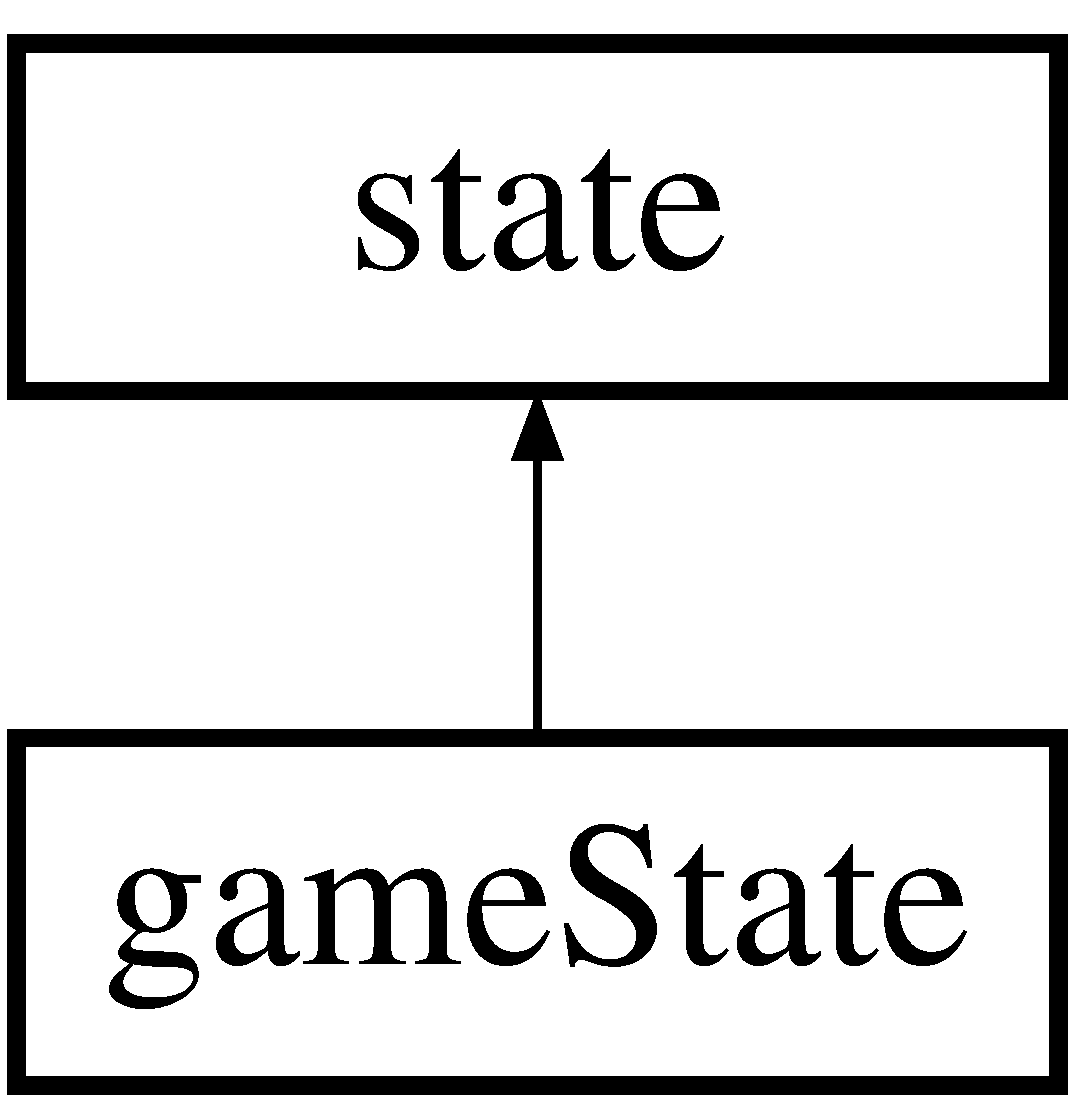
\includegraphics[height=2.000000cm]{classgame_state}
\end{center}
\end{figure}
\subsection*{Public Member Functions}
\begin{DoxyCompactItemize}
\item 
\mbox{\hyperlink{classgame_state_a5fc11204e599a3d040ab255eb303a500}{game\+State}} (sf\+::\+Render\+Window $\ast$\mbox{\hyperlink{classstate_a1bd5650a39b718f10a4efd5fb084e8b7}{window}}, std\+::stack$<$ \mbox{\hyperlink{classstate}{state}} $\ast$$>$ $\ast$\mbox{\hyperlink{classstate_af087bc20fa3153ddb682f8a223db682f}{states}})
\item 
virtual \mbox{\hyperlink{classgame_state_aff0b262e002173990841199d34803fe9}{$\sim$game\+State}} ()
\item 
void \mbox{\hyperlink{classgame_state_a5d725ba8f9cdd587f389b820c37e0020}{update\+Input}} (const float \&dt)
\item 
void \mbox{\hyperlink{classgame_state_a17b43f4eac057e2262445919ee585ca1}{update}} (const float \&dt)
\item 
void \mbox{\hyperlink{classgame_state_ac300ce2d67e175bd28335921d428b8bc}{render}} (sf\+::\+Render\+Target $\ast$target=nullptr)
\end{DoxyCompactItemize}
\subsection*{Additional Inherited Members}


\subsection{Detailed Description}
Klasa odpowiedzalna za ekran gry, stan gry. Przechowuje informacje dotycz�ce graczy. 

Definition at line 6 of file game\+State.\+h.



\subsection{Constructor \& Destructor Documentation}
\mbox{\Hypertarget{classgame_state_a5fc11204e599a3d040ab255eb303a500}\label{classgame_state_a5fc11204e599a3d040ab255eb303a500}} 
\index{game\+State@{game\+State}!game\+State@{game\+State}}
\index{game\+State@{game\+State}!game\+State@{game\+State}}
\subsubsection{\texorpdfstring{game\+State()}{gameState()}}
{\footnotesize\ttfamily game\+State\+::game\+State (\begin{DoxyParamCaption}\item[{sf\+::\+Render\+Window $\ast$}]{window,  }\item[{std\+::stack$<$ \mbox{\hyperlink{classstate}{state}} $\ast$$>$ $\ast$}]{states }\end{DoxyParamCaption})}



Definition at line 86 of file game\+State.\+cpp.

\mbox{\Hypertarget{classgame_state_aff0b262e002173990841199d34803fe9}\label{classgame_state_aff0b262e002173990841199d34803fe9}} 
\index{game\+State@{game\+State}!````~game\+State@{$\sim$game\+State}}
\index{````~game\+State@{$\sim$game\+State}!game\+State@{game\+State}}
\subsubsection{\texorpdfstring{$\sim$game\+State()}{~gameState()}}
{\footnotesize\ttfamily game\+State\+::$\sim$game\+State (\begin{DoxyParamCaption}{ }\end{DoxyParamCaption})\hspace{0.3cm}{\ttfamily [virtual]}}



Definition at line 97 of file game\+State.\+cpp.



\subsection{Member Function Documentation}
\mbox{\Hypertarget{classgame_state_ac300ce2d67e175bd28335921d428b8bc}\label{classgame_state_ac300ce2d67e175bd28335921d428b8bc}} 
\index{game\+State@{game\+State}!render@{render}}
\index{render@{render}!game\+State@{game\+State}}
\subsubsection{\texorpdfstring{render()}{render()}}
{\footnotesize\ttfamily void game\+State\+::render (\begin{DoxyParamCaption}\item[{sf\+::\+Render\+Target $\ast$}]{target = {\ttfamily nullptr} }\end{DoxyParamCaption})\hspace{0.3cm}{\ttfamily [virtual]}}

~\newline
W wersji debug zawiera pozycj� kursora myszy. Wy�wietla plansz� gry i elementy z ni� zwi�zane.

Implements \mbox{\hyperlink{classstate_a53ee61fec5b4c802f2bfafec487dfc25}{state}}.



Definition at line 138 of file game\+State.\+cpp.

\mbox{\Hypertarget{classgame_state_a17b43f4eac057e2262445919ee585ca1}\label{classgame_state_a17b43f4eac057e2262445919ee585ca1}} 
\index{game\+State@{game\+State}!update@{update}}
\index{update@{update}!game\+State@{game\+State}}
\subsubsection{\texorpdfstring{update()}{update()}}
{\footnotesize\ttfamily void game\+State\+::update (\begin{DoxyParamCaption}\item[{const float \&}]{dt }\end{DoxyParamCaption})\hspace{0.3cm}{\ttfamily [virtual]}}

~\newline
Od�wie�a stan gry co 16.\+6 milisekund, aktualizuje stan game\+State\+Board, czyli planszy oraz wci�ni�te klawisze.

Implements \mbox{\hyperlink{classstate_a02d3d37c25241efd578fdcae98ef1df8}{state}}.



Definition at line 121 of file game\+State.\+cpp.

\mbox{\Hypertarget{classgame_state_a5d725ba8f9cdd587f389b820c37e0020}\label{classgame_state_a5d725ba8f9cdd587f389b820c37e0020}} 
\index{game\+State@{game\+State}!update\+Input@{update\+Input}}
\index{update\+Input@{update\+Input}!game\+State@{game\+State}}
\subsubsection{\texorpdfstring{update\+Input()}{updateInput()}}
{\footnotesize\ttfamily void game\+State\+::update\+Input (\begin{DoxyParamCaption}\item[{const float \&}]{dt }\end{DoxyParamCaption})\hspace{0.3cm}{\ttfamily [virtual]}}



Implements \mbox{\hyperlink{classstate_a1f124791a5e818794ba0eb1ac25bff99}{state}}.



Definition at line 112 of file game\+State.\+cpp.



The documentation for this class was generated from the following files\+:\begin{DoxyCompactItemize}
\item 
\mbox{\hyperlink{game_state_8h}{game\+State.\+h}}\item 
\mbox{\hyperlink{game_state_8cpp}{game\+State.\+cpp}}\end{DoxyCompactItemize}

\hypertarget{classgui_1_1info_bar}{}\section{gui\+:\+:info\+Bar Class Reference}
\label{classgui_1_1info_bar}\index{gui\+::info\+Bar@{gui\+::info\+Bar}}


{\ttfamily \#include $<$gui.\+h$>$}

\subsection*{Public Member Functions}
\begin{DoxyCompactItemize}
\item 
\mbox{\hyperlink{classgui_1_1info_bar_a4bd267ecb3d0252502339004dcb56bac}{info\+Bar}} (float x, float y, float width, float height, sf\+::\+Color color, sf\+::\+Font $\ast$font)
\item 
virtual \mbox{\hyperlink{classgui_1_1info_bar_afe17d48a3d0a02539f0a1405d0ca07e9}{$\sim$info\+Bar}} ()
\item 
void \mbox{\hyperlink{classgui_1_1info_bar_a3141f41fcddf92856bdf55a4d938e6c9}{init\+Positions}} ()
\item 
void \mbox{\hyperlink{classgui_1_1info_bar_a64b40fe3d61a9595084410b49f1f31dc}{add\+Info}} (std\+::string position\+\_\+name, std\+::string Text)
\item 
void \mbox{\hyperlink{classgui_1_1info_bar_a20a59d50a5f9a854975b7af18890b6b7}{update\+Info}} (std\+::string text, unsigned int index)
\item 
void \mbox{\hyperlink{classgui_1_1info_bar_a2b8dd22a47431e03dec9f260f3869828}{render}} (sf\+::\+Render\+Target $\ast$target)
\end{DoxyCompactItemize}
\subsection*{Public Attributes}
\begin{DoxyCompactItemize}
\item 
std\+::map$<$ std\+::string, sf\+::\+Vector2f $>$ \mbox{\hyperlink{classgui_1_1info_bar_ac0adaab0ab1aa2e8108c726ba42316d4}{positions}}
\end{DoxyCompactItemize}


\subsection{Detailed Description}
Klasa paska informacyjnego. 

Definition at line 79 of file gui.\+h.



\subsection{Constructor \& Destructor Documentation}
\mbox{\Hypertarget{classgui_1_1info_bar_a4bd267ecb3d0252502339004dcb56bac}\label{classgui_1_1info_bar_a4bd267ecb3d0252502339004dcb56bac}} 
\index{gui\+::info\+Bar@{gui\+::info\+Bar}!info\+Bar@{info\+Bar}}
\index{info\+Bar@{info\+Bar}!gui\+::info\+Bar@{gui\+::info\+Bar}}
\subsubsection{\texorpdfstring{info\+Bar()}{infoBar()}}
{\footnotesize\ttfamily gui\+::info\+Bar\+::info\+Bar (\begin{DoxyParamCaption}\item[{float}]{x,  }\item[{float}]{y,  }\item[{float}]{width,  }\item[{float}]{height,  }\item[{sf\+::\+Color}]{color,  }\item[{sf\+::\+Font $\ast$}]{font }\end{DoxyParamCaption})}



Definition at line 176 of file gui.\+cpp.

\mbox{\Hypertarget{classgui_1_1info_bar_afe17d48a3d0a02539f0a1405d0ca07e9}\label{classgui_1_1info_bar_afe17d48a3d0a02539f0a1405d0ca07e9}} 
\index{gui\+::info\+Bar@{gui\+::info\+Bar}!````~info\+Bar@{$\sim$info\+Bar}}
\index{````~info\+Bar@{$\sim$info\+Bar}!gui\+::info\+Bar@{gui\+::info\+Bar}}
\subsubsection{\texorpdfstring{$\sim$info\+Bar()}{~infoBar()}}
{\footnotesize\ttfamily gui\+::info\+Bar\+::$\sim$info\+Bar (\begin{DoxyParamCaption}{ }\end{DoxyParamCaption})\hspace{0.3cm}{\ttfamily [virtual]}}



Definition at line 186 of file gui.\+cpp.



\subsection{Member Function Documentation}
\mbox{\Hypertarget{classgui_1_1info_bar_a64b40fe3d61a9595084410b49f1f31dc}\label{classgui_1_1info_bar_a64b40fe3d61a9595084410b49f1f31dc}} 
\index{gui\+::info\+Bar@{gui\+::info\+Bar}!add\+Info@{add\+Info}}
\index{add\+Info@{add\+Info}!gui\+::info\+Bar@{gui\+::info\+Bar}}
\subsubsection{\texorpdfstring{add\+Info()}{addInfo()}}
{\footnotesize\ttfamily void gui\+::info\+Bar\+::add\+Info (\begin{DoxyParamCaption}\item[{std\+::string}]{position\+\_\+name,  }\item[{std\+::string}]{Text }\end{DoxyParamCaption})}

~\newline
Dodaje now� informacj� do przycisku do nast�pnego wolnego slotu na danej pozycji.

Definition at line 223 of file gui.\+cpp.

\mbox{\Hypertarget{classgui_1_1info_bar_a3141f41fcddf92856bdf55a4d938e6c9}\label{classgui_1_1info_bar_a3141f41fcddf92856bdf55a4d938e6c9}} 
\index{gui\+::info\+Bar@{gui\+::info\+Bar}!init\+Positions@{init\+Positions}}
\index{init\+Positions@{init\+Positions}!gui\+::info\+Bar@{gui\+::info\+Bar}}
\subsubsection{\texorpdfstring{init\+Positions()}{initPositions()}}
{\footnotesize\ttfamily void gui\+::info\+Bar\+::init\+Positions (\begin{DoxyParamCaption}{ }\end{DoxyParamCaption})}

~\newline
Inicjalizuje sloty dla informacji. Trzy mo�liwo�ci\+: lewo, �rodek, prawo.

Definition at line 197 of file gui.\+cpp.

\mbox{\Hypertarget{classgui_1_1info_bar_a2b8dd22a47431e03dec9f260f3869828}\label{classgui_1_1info_bar_a2b8dd22a47431e03dec9f260f3869828}} 
\index{gui\+::info\+Bar@{gui\+::info\+Bar}!render@{render}}
\index{render@{render}!gui\+::info\+Bar@{gui\+::info\+Bar}}
\subsubsection{\texorpdfstring{render()}{render()}}
{\footnotesize\ttfamily void gui\+::info\+Bar\+::render (\begin{DoxyParamCaption}\item[{sf\+::\+Render\+Target $\ast$}]{target }\end{DoxyParamCaption})}



Definition at line 251 of file gui.\+cpp.

\mbox{\Hypertarget{classgui_1_1info_bar_a20a59d50a5f9a854975b7af18890b6b7}\label{classgui_1_1info_bar_a20a59d50a5f9a854975b7af18890b6b7}} 
\index{gui\+::info\+Bar@{gui\+::info\+Bar}!update\+Info@{update\+Info}}
\index{update\+Info@{update\+Info}!gui\+::info\+Bar@{gui\+::info\+Bar}}
\subsubsection{\texorpdfstring{update\+Info()}{updateInfo()}}
{\footnotesize\ttfamily void gui\+::info\+Bar\+::update\+Info (\begin{DoxyParamCaption}\item[{std\+::string}]{text,  }\item[{unsigned int}]{index }\end{DoxyParamCaption})}



Definition at line 244 of file gui.\+cpp.



\subsection{Member Data Documentation}
\mbox{\Hypertarget{classgui_1_1info_bar_ac0adaab0ab1aa2e8108c726ba42316d4}\label{classgui_1_1info_bar_ac0adaab0ab1aa2e8108c726ba42316d4}} 
\index{gui\+::info\+Bar@{gui\+::info\+Bar}!positions@{positions}}
\index{positions@{positions}!gui\+::info\+Bar@{gui\+::info\+Bar}}
\subsubsection{\texorpdfstring{positions}{positions}}
{\footnotesize\ttfamily std\+::map$<$std\+::string, sf\+::\+Vector2f$>$ gui\+::info\+Bar\+::positions}



Definition at line 95 of file gui.\+h.



The documentation for this class was generated from the following files\+:\begin{DoxyCompactItemize}
\item 
\mbox{\hyperlink{gui_8h}{gui.\+h}}\item 
\mbox{\hyperlink{gui_8cpp}{gui.\+cpp}}\end{DoxyCompactItemize}

\hypertarget{classmain_menu_state}{}\section{main\+Menu\+State Class Reference}
\label{classmain_menu_state}\index{main\+Menu\+State@{main\+Menu\+State}}


{\ttfamily \#include $<$main\+Menu\+State.\+h$>$}

Inheritance diagram for main\+Menu\+State\+:\begin{figure}[H]
\begin{center}
\leavevmode
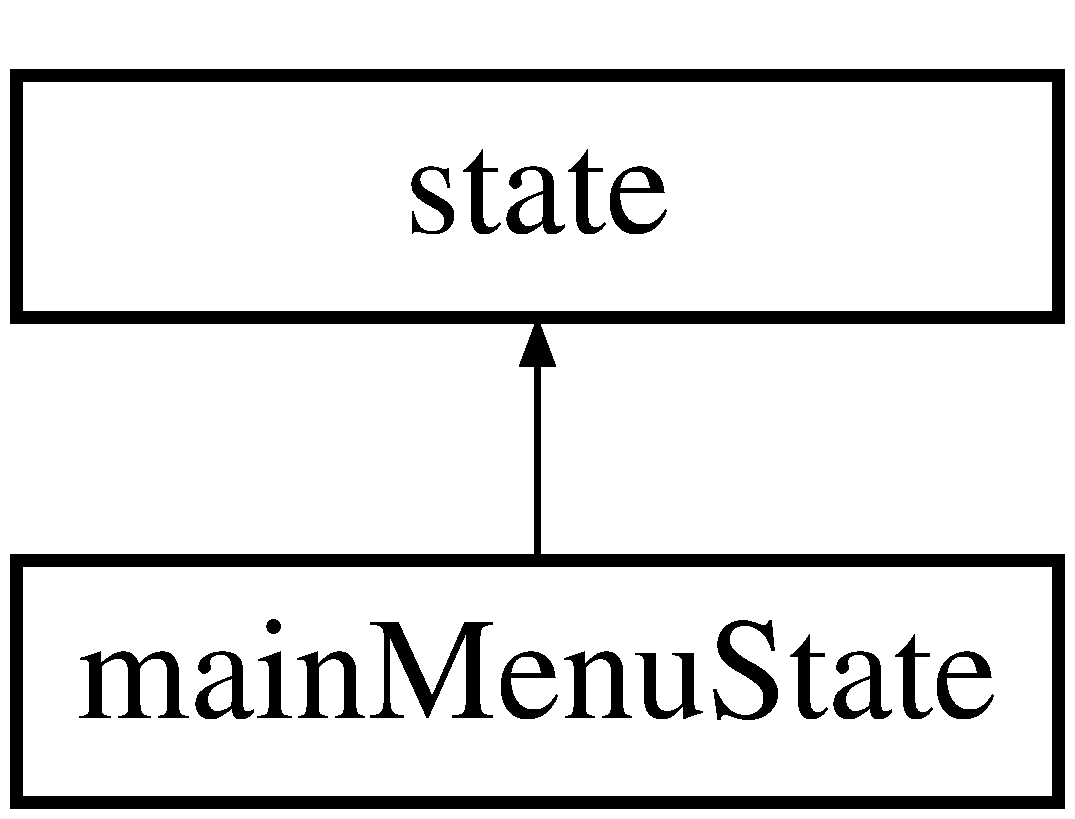
\includegraphics[height=2.000000cm]{classmain_menu_state}
\end{center}
\end{figure}
\subsection*{Public Member Functions}
\begin{DoxyCompactItemize}
\item 
\mbox{\hyperlink{classmain_menu_state_aea1bcc67a75fb1ee79695e7bce5fff3b}{main\+Menu\+State}} (sf\+::\+Render\+Window $\ast$\mbox{\hyperlink{classstate_a1bd5650a39b718f10a4efd5fb084e8b7}{window}}, std\+::stack$<$ \mbox{\hyperlink{classstate}{state}} $\ast$$>$ $\ast$\mbox{\hyperlink{classstate_af087bc20fa3153ddb682f8a223db682f}{states}})
\item 
virtual \mbox{\hyperlink{classmain_menu_state_adc83db1db1d6da9d35041d867d93916f}{$\sim$main\+Menu\+State}} ()
\item 
void \mbox{\hyperlink{classmain_menu_state_ab21e2978f82bf421c637cc74730aeca6}{update\+Input}} (const float \&dt)
\item 
void \mbox{\hyperlink{classmain_menu_state_aa3c901135c3f82e8fc20a587bb006ccc}{update\+Buttons}} (const float \&dt)
\item 
void \mbox{\hyperlink{classmain_menu_state_a24d60c6601ea578292ff8c957fca10dd}{update}} (const float \&dt)
\item 
void \mbox{\hyperlink{classmain_menu_state_ae8d65ed1c6552154715a49f24fae6b7f}{render}} (sf\+::\+Render\+Target $\ast$target=nullptr)
\item 
void \mbox{\hyperlink{classmain_menu_state_aa741f3c5e7aeb3c3c1c1bf8f99de76e3}{render\+Buttons}} (sf\+::\+Render\+Target $\ast$target=nullptr)
\end{DoxyCompactItemize}
\subsection*{Protected Member Functions}
\begin{DoxyCompactItemize}
\item 
void \mbox{\hyperlink{classmain_menu_state_a714ee680a76399e6b57c18954d045f58}{init\+Buttons}} ()
\end{DoxyCompactItemize}
\subsection*{Protected Attributes}
\begin{DoxyCompactItemize}
\item 
std\+::map$<$ std\+::string, \mbox{\hyperlink{classgui_1_1button}{gui\+::button}} $\ast$ $>$ \mbox{\hyperlink{classmain_menu_state_af1b67560d8a49f19c111a31a9d91dd41}{buttons}}
\end{DoxyCompactItemize}


\subsection{Detailed Description}
Klasa stanu menu. 

Definition at line 6 of file main\+Menu\+State.\+h.



\subsection{Constructor \& Destructor Documentation}
\mbox{\Hypertarget{classmain_menu_state_aea1bcc67a75fb1ee79695e7bce5fff3b}\label{classmain_menu_state_aea1bcc67a75fb1ee79695e7bce5fff3b}} 
\index{main\+Menu\+State@{main\+Menu\+State}!main\+Menu\+State@{main\+Menu\+State}}
\index{main\+Menu\+State@{main\+Menu\+State}!main\+Menu\+State@{main\+Menu\+State}}
\subsubsection{\texorpdfstring{main\+Menu\+State()}{mainMenuState()}}
{\footnotesize\ttfamily main\+Menu\+State\+::main\+Menu\+State (\begin{DoxyParamCaption}\item[{sf\+::\+Render\+Window $\ast$}]{window,  }\item[{std\+::stack$<$ \mbox{\hyperlink{classstate}{state}} $\ast$$>$ $\ast$}]{states }\end{DoxyParamCaption})}



Definition at line 74 of file main\+Menu\+State.\+cpp.

\mbox{\Hypertarget{classmain_menu_state_adc83db1db1d6da9d35041d867d93916f}\label{classmain_menu_state_adc83db1db1d6da9d35041d867d93916f}} 
\index{main\+Menu\+State@{main\+Menu\+State}!````~main\+Menu\+State@{$\sim$main\+Menu\+State}}
\index{````~main\+Menu\+State@{$\sim$main\+Menu\+State}!main\+Menu\+State@{main\+Menu\+State}}
\subsubsection{\texorpdfstring{$\sim$main\+Menu\+State()}{~mainMenuState()}}
{\footnotesize\ttfamily main\+Menu\+State\+::$\sim$main\+Menu\+State (\begin{DoxyParamCaption}{ }\end{DoxyParamCaption})\hspace{0.3cm}{\ttfamily [virtual]}}



Definition at line 90 of file main\+Menu\+State.\+cpp.



\subsection{Member Function Documentation}
\mbox{\Hypertarget{classmain_menu_state_a714ee680a76399e6b57c18954d045f58}\label{classmain_menu_state_a714ee680a76399e6b57c18954d045f58}} 
\index{main\+Menu\+State@{main\+Menu\+State}!init\+Buttons@{init\+Buttons}}
\index{init\+Buttons@{init\+Buttons}!main\+Menu\+State@{main\+Menu\+State}}
\subsubsection{\texorpdfstring{init\+Buttons()}{initButtons()}}
{\footnotesize\ttfamily void main\+Menu\+State\+::init\+Buttons (\begin{DoxyParamCaption}{ }\end{DoxyParamCaption})\hspace{0.3cm}{\ttfamily [protected]}}



Definition at line 29 of file main\+Menu\+State.\+cpp.

\mbox{\Hypertarget{classmain_menu_state_ae8d65ed1c6552154715a49f24fae6b7f}\label{classmain_menu_state_ae8d65ed1c6552154715a49f24fae6b7f}} 
\index{main\+Menu\+State@{main\+Menu\+State}!render@{render}}
\index{render@{render}!main\+Menu\+State@{main\+Menu\+State}}
\subsubsection{\texorpdfstring{render()}{render()}}
{\footnotesize\ttfamily void main\+Menu\+State\+::render (\begin{DoxyParamCaption}\item[{sf\+::\+Render\+Target $\ast$}]{target = {\ttfamily nullptr} }\end{DoxyParamCaption})\hspace{0.3cm}{\ttfamily [virtual]}}



Implements \mbox{\hyperlink{classstate_a53ee61fec5b4c802f2bfafec487dfc25}{state}}.



Definition at line 151 of file main\+Menu\+State.\+cpp.

\mbox{\Hypertarget{classmain_menu_state_aa741f3c5e7aeb3c3c1c1bf8f99de76e3}\label{classmain_menu_state_aa741f3c5e7aeb3c3c1c1bf8f99de76e3}} 
\index{main\+Menu\+State@{main\+Menu\+State}!render\+Buttons@{render\+Buttons}}
\index{render\+Buttons@{render\+Buttons}!main\+Menu\+State@{main\+Menu\+State}}
\subsubsection{\texorpdfstring{render\+Buttons()}{renderButtons()}}
{\footnotesize\ttfamily void main\+Menu\+State\+::render\+Buttons (\begin{DoxyParamCaption}\item[{sf\+::\+Render\+Target $\ast$}]{target = {\ttfamily nullptr} }\end{DoxyParamCaption})}



Definition at line 173 of file main\+Menu\+State.\+cpp.

\mbox{\Hypertarget{classmain_menu_state_a24d60c6601ea578292ff8c957fca10dd}\label{classmain_menu_state_a24d60c6601ea578292ff8c957fca10dd}} 
\index{main\+Menu\+State@{main\+Menu\+State}!update@{update}}
\index{update@{update}!main\+Menu\+State@{main\+Menu\+State}}
\subsubsection{\texorpdfstring{update()}{update()}}
{\footnotesize\ttfamily void main\+Menu\+State\+::update (\begin{DoxyParamCaption}\item[{const float \&}]{dt }\end{DoxyParamCaption})\hspace{0.3cm}{\ttfamily [virtual]}}



Implements \mbox{\hyperlink{classstate_a02d3d37c25241efd578fdcae98ef1df8}{state}}.



Definition at line 137 of file main\+Menu\+State.\+cpp.

\mbox{\Hypertarget{classmain_menu_state_aa3c901135c3f82e8fc20a587bb006ccc}\label{classmain_menu_state_aa3c901135c3f82e8fc20a587bb006ccc}} 
\index{main\+Menu\+State@{main\+Menu\+State}!update\+Buttons@{update\+Buttons}}
\index{update\+Buttons@{update\+Buttons}!main\+Menu\+State@{main\+Menu\+State}}
\subsubsection{\texorpdfstring{update\+Buttons()}{updateButtons()}}
{\footnotesize\ttfamily void main\+Menu\+State\+::update\+Buttons (\begin{DoxyParamCaption}\item[{const float \&}]{dt }\end{DoxyParamCaption})}



Definition at line 110 of file main\+Menu\+State.\+cpp.

\mbox{\Hypertarget{classmain_menu_state_ab21e2978f82bf421c637cc74730aeca6}\label{classmain_menu_state_ab21e2978f82bf421c637cc74730aeca6}} 
\index{main\+Menu\+State@{main\+Menu\+State}!update\+Input@{update\+Input}}
\index{update\+Input@{update\+Input}!main\+Menu\+State@{main\+Menu\+State}}
\subsubsection{\texorpdfstring{update\+Input()}{updateInput()}}
{\footnotesize\ttfamily void main\+Menu\+State\+::update\+Input (\begin{DoxyParamCaption}\item[{const float \&}]{dt }\end{DoxyParamCaption})\hspace{0.3cm}{\ttfamily [virtual]}}



Implements \mbox{\hyperlink{classstate_a1f124791a5e818794ba0eb1ac25bff99}{state}}.



Definition at line 104 of file main\+Menu\+State.\+cpp.



\subsection{Member Data Documentation}
\mbox{\Hypertarget{classmain_menu_state_af1b67560d8a49f19c111a31a9d91dd41}\label{classmain_menu_state_af1b67560d8a49f19c111a31a9d91dd41}} 
\index{main\+Menu\+State@{main\+Menu\+State}!buttons@{buttons}}
\index{buttons@{buttons}!main\+Menu\+State@{main\+Menu\+State}}
\subsubsection{\texorpdfstring{buttons}{buttons}}
{\footnotesize\ttfamily std\+::map$<$std\+::string, \mbox{\hyperlink{classgui_1_1button}{gui\+::button}}$\ast$$>$ main\+Menu\+State\+::buttons\hspace{0.3cm}{\ttfamily [protected]}}



Definition at line 27 of file main\+Menu\+State.\+h.



The documentation for this class was generated from the following files\+:\begin{DoxyCompactItemize}
\item 
\mbox{\hyperlink{main_menu_state_8h}{main\+Menu\+State.\+h}}\item 
\mbox{\hyperlink{main_menu_state_8cpp}{main\+Menu\+State.\+cpp}}\end{DoxyCompactItemize}

\hypertarget{classgui_1_1menu}{}\section{gui\+:\+:menu Class Reference}
\label{classgui_1_1menu}\index{gui\+::menu@{gui\+::menu}}


{\ttfamily \#include $<$gui.\+h$>$}

\subsection*{Public Member Functions}
\begin{DoxyCompactItemize}
\item 
\mbox{\hyperlink{classgui_1_1menu_a38c23210c7e07f41237a2bcef5b6a359}{menu}} (float x, float y, std\+::vector$<$ std\+::string $>$ button\+Names, sf\+::\+Font $\ast$font)
\item 
virtual \mbox{\hyperlink{classgui_1_1menu_a8b70ba2fd81faee45da3499f1f56e2b7}{$\sim$menu}} ()
\item 
void \mbox{\hyperlink{classgui_1_1menu_a2fe9e7d3ce3b70264eb871ce80dcbcb5}{update}} (sf\+::\+Vector2f mouse\+Pos, const float \&dt)
\item 
void \mbox{\hyperlink{classgui_1_1menu_adfe78978b42f79b996d5bc74ee94883b}{render}} (sf\+::\+Render\+Target $\ast$target)
\end{DoxyCompactItemize}
\subsection*{Public Attributes}
\begin{DoxyCompactItemize}
\item 
std\+::list$<$ \mbox{\hyperlink{classgui_1_1button}{button}} $\ast$ $>$ \mbox{\hyperlink{classgui_1_1menu_ae68ed8edb9f27b245476a0a4ab902c68}{buttons}}
\end{DoxyCompactItemize}


\subsection{Detailed Description}
Klasa menu sk�adaj�ca si� z obiekt�w klasy button. 

Definition at line 114 of file gui.\+h.



\subsection{Constructor \& Destructor Documentation}
\mbox{\Hypertarget{classgui_1_1menu_a38c23210c7e07f41237a2bcef5b6a359}\label{classgui_1_1menu_a38c23210c7e07f41237a2bcef5b6a359}} 
\index{gui\+::menu@{gui\+::menu}!menu@{menu}}
\index{menu@{menu}!gui\+::menu@{gui\+::menu}}
\subsubsection{\texorpdfstring{menu()}{menu()}}
{\footnotesize\ttfamily gui\+::menu\+::menu (\begin{DoxyParamCaption}\item[{float}]{x,  }\item[{float}]{y,  }\item[{std\+::vector$<$ std\+::string $>$}]{button\+Names,  }\item[{sf\+::\+Font $\ast$}]{font }\end{DoxyParamCaption})}

~\newline
Tworzy przyciski z podanego wektora nazw przycisk�w. Umieszcza je jeden pod drugim.

Definition at line 283 of file gui.\+cpp.

\mbox{\Hypertarget{classgui_1_1menu_a8b70ba2fd81faee45da3499f1f56e2b7}\label{classgui_1_1menu_a8b70ba2fd81faee45da3499f1f56e2b7}} 
\index{gui\+::menu@{gui\+::menu}!````~menu@{$\sim$menu}}
\index{````~menu@{$\sim$menu}!gui\+::menu@{gui\+::menu}}
\subsubsection{\texorpdfstring{$\sim$menu()}{~menu()}}
{\footnotesize\ttfamily gui\+::menu\+::$\sim$menu (\begin{DoxyParamCaption}{ }\end{DoxyParamCaption})\hspace{0.3cm}{\ttfamily [virtual]}}



Definition at line 312 of file gui.\+cpp.



\subsection{Member Function Documentation}
\mbox{\Hypertarget{classgui_1_1menu_adfe78978b42f79b996d5bc74ee94883b}\label{classgui_1_1menu_adfe78978b42f79b996d5bc74ee94883b}} 
\index{gui\+::menu@{gui\+::menu}!render@{render}}
\index{render@{render}!gui\+::menu@{gui\+::menu}}
\subsubsection{\texorpdfstring{render()}{render()}}
{\footnotesize\ttfamily void gui\+::menu\+::render (\begin{DoxyParamCaption}\item[{sf\+::\+Render\+Target $\ast$}]{target }\end{DoxyParamCaption})}



Definition at line 332 of file gui.\+cpp.

\mbox{\Hypertarget{classgui_1_1menu_a2fe9e7d3ce3b70264eb871ce80dcbcb5}\label{classgui_1_1menu_a2fe9e7d3ce3b70264eb871ce80dcbcb5}} 
\index{gui\+::menu@{gui\+::menu}!update@{update}}
\index{update@{update}!gui\+::menu@{gui\+::menu}}
\subsubsection{\texorpdfstring{update()}{update()}}
{\footnotesize\ttfamily void gui\+::menu\+::update (\begin{DoxyParamCaption}\item[{sf\+::\+Vector2f}]{mouse\+Pos,  }\item[{const float \&}]{dt }\end{DoxyParamCaption})}



Definition at line 324 of file gui.\+cpp.



\subsection{Member Data Documentation}
\mbox{\Hypertarget{classgui_1_1menu_ae68ed8edb9f27b245476a0a4ab902c68}\label{classgui_1_1menu_ae68ed8edb9f27b245476a0a4ab902c68}} 
\index{gui\+::menu@{gui\+::menu}!buttons@{buttons}}
\index{buttons@{buttons}!gui\+::menu@{gui\+::menu}}
\subsubsection{\texorpdfstring{buttons}{buttons}}
{\footnotesize\ttfamily std\+::list$<$\mbox{\hyperlink{classgui_1_1button}{button}}$\ast$$>$ gui\+::menu\+::buttons}



Definition at line 121 of file gui.\+h.



The documentation for this class was generated from the following files\+:\begin{DoxyCompactItemize}
\item 
\mbox{\hyperlink{gui_8h}{gui.\+h}}\item 
\mbox{\hyperlink{gui_8cpp}{gui.\+cpp}}\end{DoxyCompactItemize}

\hypertarget{classplayer}{}\section{player Class Reference}
\label{classplayer}\index{player@{player}}


{\ttfamily \#include $<$player.\+h$>$}

\subsection*{Public Member Functions}
\begin{DoxyCompactItemize}
\item 
\mbox{\hyperlink{classplayer_acd3dc158a3e79bf4a53737323239dbd2}{player}} (sf\+::\+Ip\+Address local\+Ip\+Address, int \mbox{\hyperlink{classplayer_a63aaa8d2259e82820437e7989f966dd3}{player\+Id}}, sf\+::\+Color \mbox{\hyperlink{classplayer_afc452b555289777d87cd6d8e18788a93}{color}})
\item 
virtual \mbox{\hyperlink{classplayer_aab5d2e47b80e0481f09ca0df8b823057}{$\sim$player}} ()
\item 
void \mbox{\hyperlink{classplayer_a201ead0a0d511b9d3d8ea02e6dc0f17a}{create\+Token}} (float x, float y, sf\+::\+Texture $\ast$texture)
\end{DoxyCompactItemize}
\subsection*{Public Attributes}
\begin{DoxyCompactItemize}
\item 
\mbox{\hyperlink{classtoken}{token}} $\ast$ \mbox{\hyperlink{classplayer_a209149cf07fc9d2d04c98cc76034c69c}{player\+Token}}
\item 
int \mbox{\hyperlink{classplayer_a63aaa8d2259e82820437e7989f966dd3}{player\+Id}}
\item 
sf\+::\+Text \mbox{\hyperlink{classplayer_a90eea2e10a265252541f3caeb14271eb}{nickname}}
\item 
sf\+::\+Color \mbox{\hyperlink{classplayer_afc452b555289777d87cd6d8e18788a93}{color}}
\item 
sf\+::\+Int64 \mbox{\hyperlink{classplayer_ab723751a3c9192f5f24c97b83acdc6b7}{last\+Dice}}
\item 
int \mbox{\hyperlink{classplayer_a1dc2aa9baa96712cce9f13cd63ceb812}{wallet}}
\end{DoxyCompactItemize}


\subsection{Detailed Description}
Klasa gracza. W domy�le ma zawiera� nickname gracza, jego adres ip, kt�ry ma slu�y� komunikacji w sieci lokalnej. Zawiera tak�e token gracza, jego stan konta oraz ostatni� ilo�� wyrzuconych oczek. 

Definition at line 6 of file player.\+h.



\subsection{Constructor \& Destructor Documentation}
\mbox{\Hypertarget{classplayer_acd3dc158a3e79bf4a53737323239dbd2}\label{classplayer_acd3dc158a3e79bf4a53737323239dbd2}} 
\index{player@{player}!player@{player}}
\index{player@{player}!player@{player}}
\subsubsection{\texorpdfstring{player()}{player()}}
{\footnotesize\ttfamily player\+::player (\begin{DoxyParamCaption}\item[{sf\+::\+Ip\+Address}]{local\+Ip\+Address,  }\item[{int}]{player\+Id,  }\item[{sf\+::\+Color}]{color }\end{DoxyParamCaption})}

~\newline
Tworzy nowego gracza z zadanym id, adresep ip, a tak�e przydzielonym mu kolorem.

Definition at line 3 of file player.\+cpp.

\mbox{\Hypertarget{classplayer_aab5d2e47b80e0481f09ca0df8b823057}\label{classplayer_aab5d2e47b80e0481f09ca0df8b823057}} 
\index{player@{player}!````~player@{$\sim$player}}
\index{````~player@{$\sim$player}!player@{player}}
\subsubsection{\texorpdfstring{$\sim$player()}{~player()}}
{\footnotesize\ttfamily player\+::$\sim$player (\begin{DoxyParamCaption}{ }\end{DoxyParamCaption})\hspace{0.3cm}{\ttfamily [virtual]}}



Definition at line 16 of file player.\+cpp.



\subsection{Member Function Documentation}
\mbox{\Hypertarget{classplayer_a201ead0a0d511b9d3d8ea02e6dc0f17a}\label{classplayer_a201ead0a0d511b9d3d8ea02e6dc0f17a}} 
\index{player@{player}!create\+Token@{create\+Token}}
\index{create\+Token@{create\+Token}!player@{player}}
\subsubsection{\texorpdfstring{create\+Token()}{createToken()}}
{\footnotesize\ttfamily void player\+::create\+Token (\begin{DoxyParamCaption}\item[{float}]{x,  }\item[{float}]{y,  }\item[{sf\+::\+Texture $\ast$}]{texture }\end{DoxyParamCaption})}

~\newline
Tworzy token dla gracza w okre�lonym miejscu.

Definition at line 22 of file player.\+cpp.



\subsection{Member Data Documentation}
\mbox{\Hypertarget{classplayer_afc452b555289777d87cd6d8e18788a93}\label{classplayer_afc452b555289777d87cd6d8e18788a93}} 
\index{player@{player}!color@{color}}
\index{color@{color}!player@{player}}
\subsubsection{\texorpdfstring{color}{color}}
{\footnotesize\ttfamily sf\+::\+Color player\+::color}



Definition at line 20 of file player.\+h.

\mbox{\Hypertarget{classplayer_ab723751a3c9192f5f24c97b83acdc6b7}\label{classplayer_ab723751a3c9192f5f24c97b83acdc6b7}} 
\index{player@{player}!last\+Dice@{last\+Dice}}
\index{last\+Dice@{last\+Dice}!player@{player}}
\subsubsection{\texorpdfstring{last\+Dice}{lastDice}}
{\footnotesize\ttfamily sf\+::\+Int64 player\+::last\+Dice}



Definition at line 21 of file player.\+h.

\mbox{\Hypertarget{classplayer_a90eea2e10a265252541f3caeb14271eb}\label{classplayer_a90eea2e10a265252541f3caeb14271eb}} 
\index{player@{player}!nickname@{nickname}}
\index{nickname@{nickname}!player@{player}}
\subsubsection{\texorpdfstring{nickname}{nickname}}
{\footnotesize\ttfamily sf\+::\+Text player\+::nickname}



Definition at line 19 of file player.\+h.

\mbox{\Hypertarget{classplayer_a63aaa8d2259e82820437e7989f966dd3}\label{classplayer_a63aaa8d2259e82820437e7989f966dd3}} 
\index{player@{player}!player\+Id@{player\+Id}}
\index{player\+Id@{player\+Id}!player@{player}}
\subsubsection{\texorpdfstring{player\+Id}{playerId}}
{\footnotesize\ttfamily int player\+::player\+Id}



Definition at line 18 of file player.\+h.

\mbox{\Hypertarget{classplayer_a209149cf07fc9d2d04c98cc76034c69c}\label{classplayer_a209149cf07fc9d2d04c98cc76034c69c}} 
\index{player@{player}!player\+Token@{player\+Token}}
\index{player\+Token@{player\+Token}!player@{player}}
\subsubsection{\texorpdfstring{player\+Token}{playerToken}}
{\footnotesize\ttfamily \mbox{\hyperlink{classtoken}{token}}$\ast$ player\+::player\+Token}



Definition at line 17 of file player.\+h.

\mbox{\Hypertarget{classplayer_a1dc2aa9baa96712cce9f13cd63ceb812}\label{classplayer_a1dc2aa9baa96712cce9f13cd63ceb812}} 
\index{player@{player}!wallet@{wallet}}
\index{wallet@{wallet}!player@{player}}
\subsubsection{\texorpdfstring{wallet}{wallet}}
{\footnotesize\ttfamily int player\+::wallet}



Definition at line 22 of file player.\+h.



The documentation for this class was generated from the following files\+:\begin{DoxyCompactItemize}
\item 
\mbox{\hyperlink{player_8h}{player.\+h}}\item 
\mbox{\hyperlink{player_8cpp}{player.\+cpp}}\end{DoxyCompactItemize}

\hypertarget{classproperty_field}{}\section{property\+Field Class Reference}
\label{classproperty_field}\index{property\+Field@{property\+Field}}


{\ttfamily \#include $<$property\+Field.\+h$>$}

Inheritance diagram for property\+Field\+:\begin{figure}[H]
\begin{center}
\leavevmode
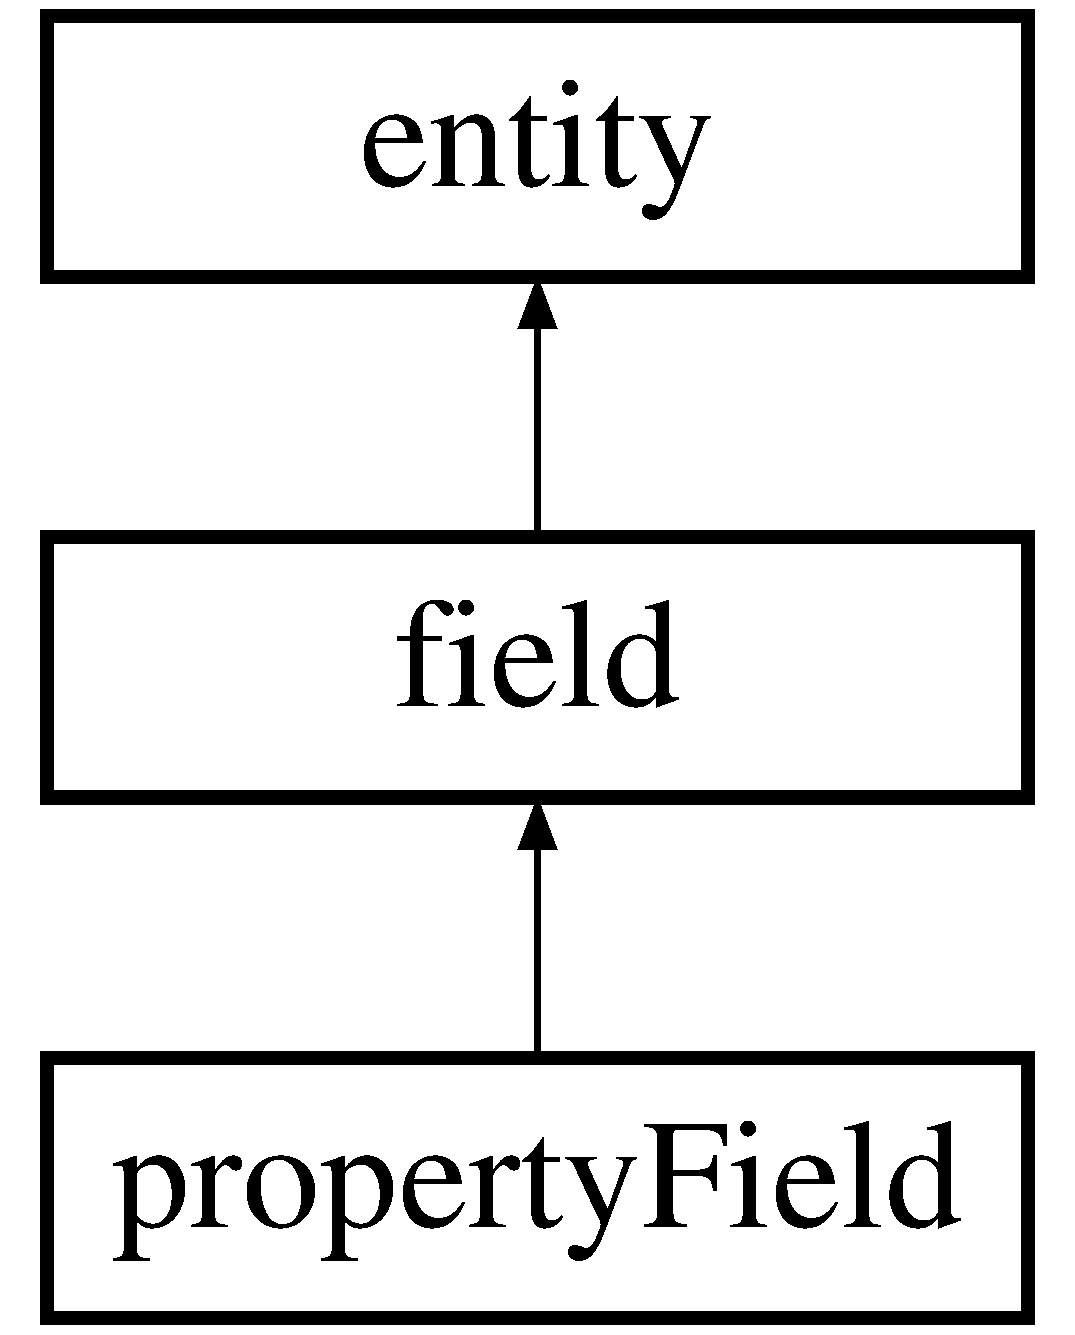
\includegraphics[height=3.000000cm]{classproperty_field}
\end{center}
\end{figure}
\subsection*{Public Member Functions}
\begin{DoxyCompactItemize}
\item 
\mbox{\hyperlink{classproperty_field_aec21e07dd2c6b7c3278924156dc7471c}{property\+Field}} (std\+::string \mbox{\hyperlink{classfield_a0fa76e9bb3e439757ad10e5f6032e1ff}{field\+Title}}, std\+::string \mbox{\hyperlink{classfield_aa1ee6124b7b2c31a8cf5b72b2a1e378e}{field\+Description}}, float x, float y, float width, float height, int rotation, sf\+::\+Color \mbox{\hyperlink{classfield_ae869b5c6466855de5bb00a0da4a738e4}{color}}, float price, float mortgage, int d\+Level\+Price, int d\+Income)
\item 
void \mbox{\hyperlink{classproperty_field_a4c2730bef86d39d723193a0b0be83255}{init\+Variables}} ()
\item 
void \mbox{\hyperlink{classproperty_field_a6d2773b5e1cdd56d496bf0fa81acff2c}{on\+Step\+Action}} (\mbox{\hyperlink{classplayer}{player}} $\ast$\mbox{\hyperlink{classfield_a52e61f57f292aadd141aecf8745b4605}{player\+On\+Field}})
\item 
void \mbox{\hyperlink{classproperty_field_a511f91ed430544655a5cab7fb8be6cc2}{buy\+Field}} (\mbox{\hyperlink{classplayer}{player}} $\ast$new\+Owner)
\item 
void \mbox{\hyperlink{classproperty_field_a32b21dcaf062135f50a674da30c707c9}{update}} (const float \&dt, sf\+::\+Vector2f mouse\+Pos)
\item 
void \mbox{\hyperlink{classproperty_field_ada6c23589e09fe31f88b75ed2ec27d11}{render}} (sf\+::\+Render\+Target $\ast$target)
\item 
virtual \mbox{\hyperlink{classproperty_field_a9f2a49b4d101d64f71336b10c402b0c5}{$\sim$property\+Field}} ()
\end{DoxyCompactItemize}
\subsection*{Additional Inherited Members}


\subsection{Detailed Description}
Pole w�asno�ci mo�liwej do nabycia. Zawiera definicj� on\+Step\+Action wy�wietlaj�c� panel z opcjami dotycz�cymi pola. 

Definition at line 5 of file property\+Field.\+h.



\subsection{Constructor \& Destructor Documentation}
\mbox{\Hypertarget{classproperty_field_aec21e07dd2c6b7c3278924156dc7471c}\label{classproperty_field_aec21e07dd2c6b7c3278924156dc7471c}} 
\index{property\+Field@{property\+Field}!property\+Field@{property\+Field}}
\index{property\+Field@{property\+Field}!property\+Field@{property\+Field}}
\subsubsection{\texorpdfstring{property\+Field()}{propertyField()}}
{\footnotesize\ttfamily property\+Field\+::property\+Field (\begin{DoxyParamCaption}\item[{std\+::string}]{field\+Title,  }\item[{std\+::string}]{field\+Description,  }\item[{float}]{x,  }\item[{float}]{y,  }\item[{float}]{width,  }\item[{float}]{height,  }\item[{int}]{rotation,  }\item[{sf\+::\+Color}]{color,  }\item[{float}]{price,  }\item[{float}]{mortgage,  }\item[{int}]{d\+Level\+Price,  }\item[{int}]{d\+Income }\end{DoxyParamCaption})}

~\newline
Tworzy pole w danym miejscu z domy�lnymi parametrami.

Definition at line 3 of file property\+Field.\+cpp.

\mbox{\Hypertarget{classproperty_field_a9f2a49b4d101d64f71336b10c402b0c5}\label{classproperty_field_a9f2a49b4d101d64f71336b10c402b0c5}} 
\index{property\+Field@{property\+Field}!````~property\+Field@{$\sim$property\+Field}}
\index{````~property\+Field@{$\sim$property\+Field}!property\+Field@{property\+Field}}
\subsubsection{\texorpdfstring{$\sim$property\+Field()}{~propertyField()}}
{\footnotesize\ttfamily property\+Field\+::$\sim$property\+Field (\begin{DoxyParamCaption}{ }\end{DoxyParamCaption})\hspace{0.3cm}{\ttfamily [virtual]}}



Definition at line 70 of file property\+Field.\+cpp.



\subsection{Member Function Documentation}
\mbox{\Hypertarget{classproperty_field_a511f91ed430544655a5cab7fb8be6cc2}\label{classproperty_field_a511f91ed430544655a5cab7fb8be6cc2}} 
\index{property\+Field@{property\+Field}!buy\+Field@{buy\+Field}}
\index{buy\+Field@{buy\+Field}!property\+Field@{property\+Field}}
\subsubsection{\texorpdfstring{buy\+Field()}{buyField()}}
{\footnotesize\ttfamily void property\+Field\+::buy\+Field (\begin{DoxyParamCaption}\item[{\mbox{\hyperlink{classplayer}{player}} $\ast$}]{new\+Owner }\end{DoxyParamCaption})}

~\newline
Zmienia w�a�ciciela niezakupionego pola i pobiera op�at�.

Definition at line 228 of file property\+Field.\+cpp.

\mbox{\Hypertarget{classproperty_field_a4c2730bef86d39d723193a0b0be83255}\label{classproperty_field_a4c2730bef86d39d723193a0b0be83255}} 
\index{property\+Field@{property\+Field}!init\+Variables@{init\+Variables}}
\index{init\+Variables@{init\+Variables}!property\+Field@{property\+Field}}
\subsubsection{\texorpdfstring{init\+Variables()}{initVariables()}}
{\footnotesize\ttfamily void property\+Field\+::init\+Variables (\begin{DoxyParamCaption}{ }\end{DoxyParamCaption})}



Definition at line 81 of file property\+Field.\+cpp.

\mbox{\Hypertarget{classproperty_field_a6d2773b5e1cdd56d496bf0fa81acff2c}\label{classproperty_field_a6d2773b5e1cdd56d496bf0fa81acff2c}} 
\index{property\+Field@{property\+Field}!on\+Step\+Action@{on\+Step\+Action}}
\index{on\+Step\+Action@{on\+Step\+Action}!property\+Field@{property\+Field}}
\subsubsection{\texorpdfstring{on\+Step\+Action()}{onStepAction()}}
{\footnotesize\ttfamily void property\+Field\+::on\+Step\+Action (\begin{DoxyParamCaption}\item[{\mbox{\hyperlink{classplayer}{player}} $\ast$}]{player\+On\+Field }\end{DoxyParamCaption})\hspace{0.3cm}{\ttfamily [virtual]}}

~\newline
W zale�no�ci od tego, czy gracz jest w�a�cicielem, potencjalnym nabywc�, czy klientem przeprowadza r�ne akcje.

Implements \mbox{\hyperlink{classfield_a940f9ab5e5a33ce71f77c88c5b312300}{field}}.



Definition at line 166 of file property\+Field.\+cpp.

\mbox{\Hypertarget{classproperty_field_ada6c23589e09fe31f88b75ed2ec27d11}\label{classproperty_field_ada6c23589e09fe31f88b75ed2ec27d11}} 
\index{property\+Field@{property\+Field}!render@{render}}
\index{render@{render}!property\+Field@{property\+Field}}
\subsubsection{\texorpdfstring{render()}{render()}}
{\footnotesize\ttfamily void property\+Field\+::render (\begin{DoxyParamCaption}\item[{sf\+::\+Render\+Target $\ast$}]{target }\end{DoxyParamCaption})\hspace{0.3cm}{\ttfamily [virtual]}}

~\newline
Je�li istnieje menu to renderuje menu i pole. Je�li nie to tylko pole.

Reimplemented from \mbox{\hyperlink{classfield_a3b2cdb0e289aa1b47ce79360b975f6a9}{field}}.



Definition at line 241 of file property\+Field.\+cpp.

\mbox{\Hypertarget{classproperty_field_a32b21dcaf062135f50a674da30c707c9}\label{classproperty_field_a32b21dcaf062135f50a674da30c707c9}} 
\index{property\+Field@{property\+Field}!update@{update}}
\index{update@{update}!property\+Field@{property\+Field}}
\subsubsection{\texorpdfstring{update()}{update()}}
{\footnotesize\ttfamily void property\+Field\+::update (\begin{DoxyParamCaption}\item[{const float \&}]{dt,  }\item[{sf\+::\+Vector2f}]{mouse\+Pos }\end{DoxyParamCaption})\hspace{0.3cm}{\ttfamily [virtual]}}



Reimplemented from \mbox{\hyperlink{classfield_a526cc088056de1c0efdcf55fe1062e78}{field}}.



Definition at line 94 of file property\+Field.\+cpp.



The documentation for this class was generated from the following files\+:\begin{DoxyCompactItemize}
\item 
\mbox{\hyperlink{property_field_8h}{property\+Field.\+h}}\item 
\mbox{\hyperlink{property_field_8cpp}{property\+Field.\+cpp}}\end{DoxyCompactItemize}

\hypertarget{classstate}{}\section{state Class Reference}
\label{classstate}\index{state@{state}}


{\ttfamily \#include $<$state.\+h$>$}

Inheritance diagram for state\+:\begin{figure}[H]
\begin{center}
\leavevmode
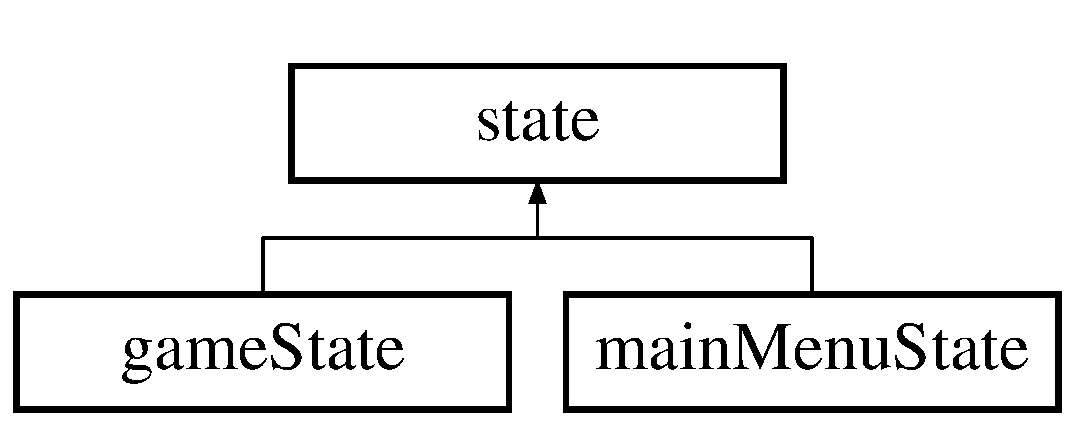
\includegraphics[height=2.000000cm]{classstate}
\end{center}
\end{figure}
\subsection*{Public Member Functions}
\begin{DoxyCompactItemize}
\item 
\mbox{\hyperlink{classstate_a1258e58ed076a4c699939cfec000b2e5}{state}} (sf\+::\+Render\+Window $\ast$\mbox{\hyperlink{classstate_a1bd5650a39b718f10a4efd5fb084e8b7}{window}}, std\+::stack$<$ \mbox{\hyperlink{classstate}{state}} $\ast$$>$ $\ast$\mbox{\hyperlink{classstate_af087bc20fa3153ddb682f8a223db682f}{states}})
\item 
virtual \mbox{\hyperlink{classstate_a60216b51b01ca0ebe9786ec2da66568f}{$\sim$state}} ()
\item 
const bool \& \mbox{\hyperlink{classstate_aa210cd4c925e8e3fa1f243f28d452de4}{get\+Quit}} () const
\item 
virtual void \mbox{\hyperlink{classstate_aa5712fe50b3d9cca1e3b6259b24e6a6d}{end\+State}} ()
\item 
virtual void \mbox{\hyperlink{classstate_a1f124791a5e818794ba0eb1ac25bff99}{update\+Input}} (const float \&dt)=0
\item 
virtual void \mbox{\hyperlink{classstate_ab2eb0cbe16984473fd8ed5d09bc30ddc}{update\+Mouse\+Position}} ()
\item 
virtual void \mbox{\hyperlink{classstate_a02d3d37c25241efd578fdcae98ef1df8}{update}} (const float \&dt)=0
\item 
virtual void \mbox{\hyperlink{classstate_a53ee61fec5b4c802f2bfafec487dfc25}{render}} (sf\+::\+Render\+Target $\ast$target=nullptr)=0
\end{DoxyCompactItemize}
\subsection*{Protected Member Functions}
\begin{DoxyCompactItemize}
\item 
virtual void \mbox{\hyperlink{classstate_a2bd58f6cc06ea368b1024f4e488c119d}{init\+Fonts}} ()
\item 
virtual sf\+::\+Texture \mbox{\hyperlink{classstate_af2af4d6fabe71ee689fa9b2a998a0cea}{load\+Texture}} (std\+::string location)
\end{DoxyCompactItemize}
\subsection*{Protected Attributes}
\begin{DoxyCompactItemize}
\item 
sf\+::\+Render\+Window $\ast$ \mbox{\hyperlink{classstate_a1bd5650a39b718f10a4efd5fb084e8b7}{window}}
\item 
sf\+::\+Vector2i \mbox{\hyperlink{classstate_afbff51e4f7a097f7d34e770d6172fe1e}{mouse\+Pos\+Screen}}
\item 
sf\+::\+Vector2i \mbox{\hyperlink{classstate_aa57df366f247d465925d7c9cf2448ebd}{mouse\+Pos\+Window}}
\item 
sf\+::\+Vector2f \mbox{\hyperlink{classstate_a421c0ac741ff28f1165f0ba4080bce4e}{mouse\+Pos\+View}}
\item 
std\+::stack$<$ \mbox{\hyperlink{classstate}{state}} $\ast$ $>$ $\ast$ \mbox{\hyperlink{classstate_af087bc20fa3153ddb682f8a223db682f}{states}}
\item 
std\+::map$<$ std\+::string, sf\+::\+Texture $>$ \mbox{\hyperlink{classstate_a33ff2365e5091d6ab61a8a7ac710817e}{textures}}
\item 
bool \mbox{\hyperlink{classstate_ab018de9ab34bc5e635baf904d3dfb4e9}{quit}}
\item 
sf\+::\+Font \mbox{\hyperlink{classstate_a7d48367b0a0a40795ecae59764d93f13}{font}}
\end{DoxyCompactItemize}


\subsection{Detailed Description}
Abstrakcyjna klasa stanu. Pozwala na tworzenie nowych ekran�w takich jak menu, stan gry, kt�re s� nowymi stanami. 

Definition at line 20 of file state.\+h.



\subsection{Constructor \& Destructor Documentation}
\mbox{\Hypertarget{classstate_a1258e58ed076a4c699939cfec000b2e5}\label{classstate_a1258e58ed076a4c699939cfec000b2e5}} 
\index{state@{state}!state@{state}}
\index{state@{state}!state@{state}}
\subsubsection{\texorpdfstring{state()}{state()}}
{\footnotesize\ttfamily state\+::state (\begin{DoxyParamCaption}\item[{sf\+::\+Render\+Window $\ast$}]{window,  }\item[{std\+::stack$<$ \mbox{\hyperlink{classstate}{state}} $\ast$$>$ $\ast$}]{states }\end{DoxyParamCaption})}

~\newline
Inicjuje czcionk� oraz inicjalizuje zmienne. Przekazuje wska�nik na stos stan�w.

Definition at line 30 of file state.\+cpp.

\mbox{\Hypertarget{classstate_a60216b51b01ca0ebe9786ec2da66568f}\label{classstate_a60216b51b01ca0ebe9786ec2da66568f}} 
\index{state@{state}!````~state@{$\sim$state}}
\index{````~state@{$\sim$state}!state@{state}}
\subsubsection{\texorpdfstring{$\sim$state()}{~state()}}
{\footnotesize\ttfamily state\+::$\sim$state (\begin{DoxyParamCaption}{ }\end{DoxyParamCaption})\hspace{0.3cm}{\ttfamily [virtual]}}



Definition at line 44 of file state.\+cpp.



\subsection{Member Function Documentation}
\mbox{\Hypertarget{classstate_aa5712fe50b3d9cca1e3b6259b24e6a6d}\label{classstate_aa5712fe50b3d9cca1e3b6259b24e6a6d}} 
\index{state@{state}!end\+State@{end\+State}}
\index{end\+State@{end\+State}!state@{state}}
\subsubsection{\texorpdfstring{end\+State()}{endState()}}
{\footnotesize\ttfamily void state\+::end\+State (\begin{DoxyParamCaption}{ }\end{DoxyParamCaption})\hspace{0.3cm}{\ttfamily [virtual]}}

~\newline
Zmienai atrybut quit na true i prowadzi do usuni�cia stanu.

Definition at line 58 of file state.\+cpp.

\mbox{\Hypertarget{classstate_aa210cd4c925e8e3fa1f243f28d452de4}\label{classstate_aa210cd4c925e8e3fa1f243f28d452de4}} 
\index{state@{state}!get\+Quit@{get\+Quit}}
\index{get\+Quit@{get\+Quit}!state@{state}}
\subsubsection{\texorpdfstring{get\+Quit()}{getQuit()}}
{\footnotesize\ttfamily const bool \& state\+::get\+Quit (\begin{DoxyParamCaption}{ }\end{DoxyParamCaption}) const}



Definition at line 50 of file state.\+cpp.

\mbox{\Hypertarget{classstate_a2bd58f6cc06ea368b1024f4e488c119d}\label{classstate_a2bd58f6cc06ea368b1024f4e488c119d}} 
\index{state@{state}!init\+Fonts@{init\+Fonts}}
\index{init\+Fonts@{init\+Fonts}!state@{state}}
\subsubsection{\texorpdfstring{init\+Fonts()}{initFonts()}}
{\footnotesize\ttfamily void state\+::init\+Fonts (\begin{DoxyParamCaption}{ }\end{DoxyParamCaption})\hspace{0.3cm}{\ttfamily [protected]}, {\ttfamily [virtual]}}

~\newline
Inicjuje czcionk� z lokalizacji\+: fonts/\+M\+O\+N\+O\+P\+O\+L\+Y\+\_\+\+I\+N\+L\+I\+N\+E.\+T\+TF.

Definition at line 2 of file state.\+cpp.

\mbox{\Hypertarget{classstate_af2af4d6fabe71ee689fa9b2a998a0cea}\label{classstate_af2af4d6fabe71ee689fa9b2a998a0cea}} 
\index{state@{state}!load\+Texture@{load\+Texture}}
\index{load\+Texture@{load\+Texture}!state@{state}}
\subsubsection{\texorpdfstring{load\+Texture()}{loadTexture()}}
{\footnotesize\ttfamily sf\+::\+Texture state\+::load\+Texture (\begin{DoxyParamCaption}\item[{std\+::string}]{location }\end{DoxyParamCaption})\hspace{0.3cm}{\ttfamily [protected]}, {\ttfamily [virtual]}}

~\newline
Inicjuje tekstury z lokalizacji\+: resources/images/errors/none.\+png.

Definition at line 14 of file state.\+cpp.

\mbox{\Hypertarget{classstate_a53ee61fec5b4c802f2bfafec487dfc25}\label{classstate_a53ee61fec5b4c802f2bfafec487dfc25}} 
\index{state@{state}!render@{render}}
\index{render@{render}!state@{state}}
\subsubsection{\texorpdfstring{render()}{render()}}
{\footnotesize\ttfamily virtual void state\+::render (\begin{DoxyParamCaption}\item[{sf\+::\+Render\+Target $\ast$}]{target = {\ttfamily nullptr} }\end{DoxyParamCaption})\hspace{0.3cm}{\ttfamily [pure virtual]}}



Implemented in \mbox{\hyperlink{classmain_menu_state_ae8d65ed1c6552154715a49f24fae6b7f}{main\+Menu\+State}}, and \mbox{\hyperlink{classgame_state_ac300ce2d67e175bd28335921d428b8bc}{game\+State}}.

\mbox{\Hypertarget{classstate_a02d3d37c25241efd578fdcae98ef1df8}\label{classstate_a02d3d37c25241efd578fdcae98ef1df8}} 
\index{state@{state}!update@{update}}
\index{update@{update}!state@{state}}
\subsubsection{\texorpdfstring{update()}{update()}}
{\footnotesize\ttfamily virtual void state\+::update (\begin{DoxyParamCaption}\item[{const float \&}]{dt }\end{DoxyParamCaption})\hspace{0.3cm}{\ttfamily [pure virtual]}}



Implemented in \mbox{\hyperlink{classmain_menu_state_a24d60c6601ea578292ff8c957fca10dd}{main\+Menu\+State}}, and \mbox{\hyperlink{classgame_state_a17b43f4eac057e2262445919ee585ca1}{game\+State}}.

\mbox{\Hypertarget{classstate_a1f124791a5e818794ba0eb1ac25bff99}\label{classstate_a1f124791a5e818794ba0eb1ac25bff99}} 
\index{state@{state}!update\+Input@{update\+Input}}
\index{update\+Input@{update\+Input}!state@{state}}
\subsubsection{\texorpdfstring{update\+Input()}{updateInput()}}
{\footnotesize\ttfamily virtual void state\+::update\+Input (\begin{DoxyParamCaption}\item[{const float \&}]{dt }\end{DoxyParamCaption})\hspace{0.3cm}{\ttfamily [pure virtual]}}



Implemented in \mbox{\hyperlink{classmain_menu_state_ab21e2978f82bf421c637cc74730aeca6}{main\+Menu\+State}}, and \mbox{\hyperlink{classgame_state_a5d725ba8f9cdd587f389b820c37e0020}{game\+State}}.

\mbox{\Hypertarget{classstate_ab2eb0cbe16984473fd8ed5d09bc30ddc}\label{classstate_ab2eb0cbe16984473fd8ed5d09bc30ddc}} 
\index{state@{state}!update\+Mouse\+Position@{update\+Mouse\+Position}}
\index{update\+Mouse\+Position@{update\+Mouse\+Position}!state@{state}}
\subsubsection{\texorpdfstring{update\+Mouse\+Position()}{updateMousePosition()}}
{\footnotesize\ttfamily void state\+::update\+Mouse\+Position (\begin{DoxyParamCaption}{ }\end{DoxyParamCaption})\hspace{0.3cm}{\ttfamily [virtual]}}



Definition at line 66 of file state.\+cpp.



\subsection{Member Data Documentation}
\mbox{\Hypertarget{classstate_a7d48367b0a0a40795ecae59764d93f13}\label{classstate_a7d48367b0a0a40795ecae59764d93f13}} 
\index{state@{state}!font@{font}}
\index{font@{font}!state@{state}}
\subsubsection{\texorpdfstring{font}{font}}
{\footnotesize\ttfamily sf\+::\+Font state\+::font\hspace{0.3cm}{\ttfamily [protected]}}



Definition at line 56 of file state.\+h.

\mbox{\Hypertarget{classstate_afbff51e4f7a097f7d34e770d6172fe1e}\label{classstate_afbff51e4f7a097f7d34e770d6172fe1e}} 
\index{state@{state}!mouse\+Pos\+Screen@{mouse\+Pos\+Screen}}
\index{mouse\+Pos\+Screen@{mouse\+Pos\+Screen}!state@{state}}
\subsubsection{\texorpdfstring{mouse\+Pos\+Screen}{mousePosScreen}}
{\footnotesize\ttfamily sf\+::\+Vector2i state\+::mouse\+Pos\+Screen\hspace{0.3cm}{\ttfamily [protected]}}



Definition at line 37 of file state.\+h.

\mbox{\Hypertarget{classstate_a421c0ac741ff28f1165f0ba4080bce4e}\label{classstate_a421c0ac741ff28f1165f0ba4080bce4e}} 
\index{state@{state}!mouse\+Pos\+View@{mouse\+Pos\+View}}
\index{mouse\+Pos\+View@{mouse\+Pos\+View}!state@{state}}
\subsubsection{\texorpdfstring{mouse\+Pos\+View}{mousePosView}}
{\footnotesize\ttfamily sf\+::\+Vector2f state\+::mouse\+Pos\+View\hspace{0.3cm}{\ttfamily [protected]}}



Definition at line 39 of file state.\+h.

\mbox{\Hypertarget{classstate_aa57df366f247d465925d7c9cf2448ebd}\label{classstate_aa57df366f247d465925d7c9cf2448ebd}} 
\index{state@{state}!mouse\+Pos\+Window@{mouse\+Pos\+Window}}
\index{mouse\+Pos\+Window@{mouse\+Pos\+Window}!state@{state}}
\subsubsection{\texorpdfstring{mouse\+Pos\+Window}{mousePosWindow}}
{\footnotesize\ttfamily sf\+::\+Vector2i state\+::mouse\+Pos\+Window\hspace{0.3cm}{\ttfamily [protected]}}



Definition at line 38 of file state.\+h.

\mbox{\Hypertarget{classstate_ab018de9ab34bc5e635baf904d3dfb4e9}\label{classstate_ab018de9ab34bc5e635baf904d3dfb4e9}} 
\index{state@{state}!quit@{quit}}
\index{quit@{quit}!state@{state}}
\subsubsection{\texorpdfstring{quit}{quit}}
{\footnotesize\ttfamily bool state\+::quit\hspace{0.3cm}{\ttfamily [protected]}}



Definition at line 55 of file state.\+h.

\mbox{\Hypertarget{classstate_af087bc20fa3153ddb682f8a223db682f}\label{classstate_af087bc20fa3153ddb682f8a223db682f}} 
\index{state@{state}!states@{states}}
\index{states@{states}!state@{state}}
\subsubsection{\texorpdfstring{states}{states}}
{\footnotesize\ttfamily std\+::stack$<$\mbox{\hyperlink{classstate}{state}}$\ast$$>$$\ast$ state\+::states\hspace{0.3cm}{\ttfamily [protected]}}



Definition at line 41 of file state.\+h.

\mbox{\Hypertarget{classstate_a33ff2365e5091d6ab61a8a7ac710817e}\label{classstate_a33ff2365e5091d6ab61a8a7ac710817e}} 
\index{state@{state}!textures@{textures}}
\index{textures@{textures}!state@{state}}
\subsubsection{\texorpdfstring{textures}{textures}}
{\footnotesize\ttfamily std\+::map$<$std\+::string, sf\+::\+Texture$>$ state\+::textures\hspace{0.3cm}{\ttfamily [protected]}}



Definition at line 46 of file state.\+h.

\mbox{\Hypertarget{classstate_a1bd5650a39b718f10a4efd5fb084e8b7}\label{classstate_a1bd5650a39b718f10a4efd5fb084e8b7}} 
\index{state@{state}!window@{window}}
\index{window@{window}!state@{state}}
\subsubsection{\texorpdfstring{window}{window}}
{\footnotesize\ttfamily sf\+::\+Render\+Window$\ast$ state\+::window\hspace{0.3cm}{\ttfamily [protected]}}



Definition at line 36 of file state.\+h.



The documentation for this class was generated from the following files\+:\begin{DoxyCompactItemize}
\item 
\mbox{\hyperlink{state_8h}{state.\+h}}\item 
\mbox{\hyperlink{state_8cpp}{state.\+cpp}}\end{DoxyCompactItemize}

\hypertarget{classtext_box}{}\section{text\+Box Class Reference}
\label{classtext_box}\index{text\+Box@{text\+Box}}


{\ttfamily \#include $<$text\+Box.\+h$>$}

\subsection*{Public Member Functions}
\begin{DoxyCompactItemize}
\item 
\mbox{\hyperlink{classtext_box_ae2978707ad54e9a02106694370acfe6f}{text\+Box}} ()
\item 
\mbox{\hyperlink{classtext_box_a5a70337146669e9bfadb15d16f67db37}{text\+Box}} (int size, sf\+::\+Color color, bool sel)
\item 
void \mbox{\hyperlink{classtext_box_a390fb8374ec6fec5dc3a71e9a4257553}{set\+Font}} (sf\+::\+Font \&font)
\item 
void \mbox{\hyperlink{classtext_box_ae2103e20eb1adeb3bb5a29cc50b511b9}{set\+Position}} (sf\+::\+Vector2f pos)
\item 
void \mbox{\hyperlink{classtext_box_a481f81251c418b55fe78e230fcc1bc75}{set\+Limit}} (bool ToF)
\item 
void \mbox{\hyperlink{classtext_box_adbcf45bbab4faadc172e419da752484b}{set\+Limit}} (bool ToF, int lim)
\item 
void \mbox{\hyperlink{classtext_box_a9b5a0f5e721811f899659436ff5707d0}{is\+Tracker}} (bool ToF)
\item 
void \mbox{\hyperlink{classtext_box_ad119049c6dae381322ba4ff22d9eda42}{set\+Selected}} (bool sel)
\item 
std\+::string \mbox{\hyperlink{classtext_box_a71136cb45321e5620ef8ab9e1ace7348}{get\+Text}} ()
\item 
void \mbox{\hyperlink{classtext_box_a27b3756c0fabe55db09145a30adb793e}{draw\+To}} (sf\+::\+Render\+Window \&window)
\item 
void \mbox{\hyperlink{classtext_box_a6ffbf16c973f4a49fed5661813ae9cce}{typed\+On}} (sf\+::\+Event input)
\end{DoxyCompactItemize}


\subsection{Detailed Description}


Definition at line 13 of file text\+Box.\+h.



\subsection{Constructor \& Destructor Documentation}
\mbox{\Hypertarget{classtext_box_ae2978707ad54e9a02106694370acfe6f}\label{classtext_box_ae2978707ad54e9a02106694370acfe6f}} 
\index{text\+Box@{text\+Box}!text\+Box@{text\+Box}}
\index{text\+Box@{text\+Box}!text\+Box@{text\+Box}}
\subsubsection{\texorpdfstring{text\+Box()}{textBox()}\hspace{0.1cm}{\footnotesize\ttfamily [1/2]}}
{\footnotesize\ttfamily text\+Box\+::text\+Box (\begin{DoxyParamCaption}{ }\end{DoxyParamCaption})\hspace{0.3cm}{\ttfamily [inline]}}



Definition at line 16 of file text\+Box.\+h.

\mbox{\Hypertarget{classtext_box_a5a70337146669e9bfadb15d16f67db37}\label{classtext_box_a5a70337146669e9bfadb15d16f67db37}} 
\index{text\+Box@{text\+Box}!text\+Box@{text\+Box}}
\index{text\+Box@{text\+Box}!text\+Box@{text\+Box}}
\subsubsection{\texorpdfstring{text\+Box()}{textBox()}\hspace{0.1cm}{\footnotesize\ttfamily [2/2]}}
{\footnotesize\ttfamily text\+Box\+::text\+Box (\begin{DoxyParamCaption}\item[{int}]{size,  }\item[{sf\+::\+Color}]{color,  }\item[{bool}]{sel }\end{DoxyParamCaption})\hspace{0.3cm}{\ttfamily [inline]}}



Definition at line 18 of file text\+Box.\+h.



\subsection{Member Function Documentation}
\mbox{\Hypertarget{classtext_box_a27b3756c0fabe55db09145a30adb793e}\label{classtext_box_a27b3756c0fabe55db09145a30adb793e}} 
\index{text\+Box@{text\+Box}!draw\+To@{draw\+To}}
\index{draw\+To@{draw\+To}!text\+Box@{text\+Box}}
\subsubsection{\texorpdfstring{draw\+To()}{drawTo()}}
{\footnotesize\ttfamily void text\+Box\+::draw\+To (\begin{DoxyParamCaption}\item[{sf\+::\+Render\+Window \&}]{window }\end{DoxyParamCaption})\hspace{0.3cm}{\ttfamily [inline]}}



Definition at line 77 of file text\+Box.\+h.

\mbox{\Hypertarget{classtext_box_a71136cb45321e5620ef8ab9e1ace7348}\label{classtext_box_a71136cb45321e5620ef8ab9e1ace7348}} 
\index{text\+Box@{text\+Box}!get\+Text@{get\+Text}}
\index{get\+Text@{get\+Text}!text\+Box@{text\+Box}}
\subsubsection{\texorpdfstring{get\+Text()}{getText()}}
{\footnotesize\ttfamily std\+::string text\+Box\+::get\+Text (\begin{DoxyParamCaption}{ }\end{DoxyParamCaption})\hspace{0.3cm}{\ttfamily [inline]}}



Definition at line 73 of file text\+Box.\+h.

\mbox{\Hypertarget{classtext_box_a9b5a0f5e721811f899659436ff5707d0}\label{classtext_box_a9b5a0f5e721811f899659436ff5707d0}} 
\index{text\+Box@{text\+Box}!is\+Tracker@{is\+Tracker}}
\index{is\+Tracker@{is\+Tracker}!text\+Box@{text\+Box}}
\subsubsection{\texorpdfstring{is\+Tracker()}{isTracker()}}
{\footnotesize\ttfamily void text\+Box\+::is\+Tracker (\begin{DoxyParamCaption}\item[{bool}]{ToF }\end{DoxyParamCaption})\hspace{0.3cm}{\ttfamily [inline]}}



Definition at line 47 of file text\+Box.\+h.

\mbox{\Hypertarget{classtext_box_a390fb8374ec6fec5dc3a71e9a4257553}\label{classtext_box_a390fb8374ec6fec5dc3a71e9a4257553}} 
\index{text\+Box@{text\+Box}!set\+Font@{set\+Font}}
\index{set\+Font@{set\+Font}!text\+Box@{text\+Box}}
\subsubsection{\texorpdfstring{set\+Font()}{setFont()}}
{\footnotesize\ttfamily void text\+Box\+::set\+Font (\begin{DoxyParamCaption}\item[{sf\+::\+Font \&}]{font }\end{DoxyParamCaption})\hspace{0.3cm}{\ttfamily [inline]}}



Definition at line 29 of file text\+Box.\+h.

\mbox{\Hypertarget{classtext_box_a481f81251c418b55fe78e230fcc1bc75}\label{classtext_box_a481f81251c418b55fe78e230fcc1bc75}} 
\index{text\+Box@{text\+Box}!set\+Limit@{set\+Limit}}
\index{set\+Limit@{set\+Limit}!text\+Box@{text\+Box}}
\subsubsection{\texorpdfstring{set\+Limit()}{setLimit()}\hspace{0.1cm}{\footnotesize\ttfamily [1/2]}}
{\footnotesize\ttfamily void text\+Box\+::set\+Limit (\begin{DoxyParamCaption}\item[{bool}]{ToF }\end{DoxyParamCaption})\hspace{0.3cm}{\ttfamily [inline]}}



Definition at line 38 of file text\+Box.\+h.

\mbox{\Hypertarget{classtext_box_adbcf45bbab4faadc172e419da752484b}\label{classtext_box_adbcf45bbab4faadc172e419da752484b}} 
\index{text\+Box@{text\+Box}!set\+Limit@{set\+Limit}}
\index{set\+Limit@{set\+Limit}!text\+Box@{text\+Box}}
\subsubsection{\texorpdfstring{set\+Limit()}{setLimit()}\hspace{0.1cm}{\footnotesize\ttfamily [2/2]}}
{\footnotesize\ttfamily void text\+Box\+::set\+Limit (\begin{DoxyParamCaption}\item[{bool}]{ToF,  }\item[{int}]{lim }\end{DoxyParamCaption})\hspace{0.3cm}{\ttfamily [inline]}}



Definition at line 42 of file text\+Box.\+h.

\mbox{\Hypertarget{classtext_box_ae2103e20eb1adeb3bb5a29cc50b511b9}\label{classtext_box_ae2103e20eb1adeb3bb5a29cc50b511b9}} 
\index{text\+Box@{text\+Box}!set\+Position@{set\+Position}}
\index{set\+Position@{set\+Position}!text\+Box@{text\+Box}}
\subsubsection{\texorpdfstring{set\+Position()}{setPosition()}}
{\footnotesize\ttfamily void text\+Box\+::set\+Position (\begin{DoxyParamCaption}\item[{sf\+::\+Vector2f}]{pos }\end{DoxyParamCaption})\hspace{0.3cm}{\ttfamily [inline]}}



Definition at line 34 of file text\+Box.\+h.

\mbox{\Hypertarget{classtext_box_ad119049c6dae381322ba4ff22d9eda42}\label{classtext_box_ad119049c6dae381322ba4ff22d9eda42}} 
\index{text\+Box@{text\+Box}!set\+Selected@{set\+Selected}}
\index{set\+Selected@{set\+Selected}!text\+Box@{text\+Box}}
\subsubsection{\texorpdfstring{set\+Selected()}{setSelected()}}
{\footnotesize\ttfamily void text\+Box\+::set\+Selected (\begin{DoxyParamCaption}\item[{bool}]{sel }\end{DoxyParamCaption})\hspace{0.3cm}{\ttfamily [inline]}}



Definition at line 62 of file text\+Box.\+h.

\mbox{\Hypertarget{classtext_box_a6ffbf16c973f4a49fed5661813ae9cce}\label{classtext_box_a6ffbf16c973f4a49fed5661813ae9cce}} 
\index{text\+Box@{text\+Box}!typed\+On@{typed\+On}}
\index{typed\+On@{typed\+On}!text\+Box@{text\+Box}}
\subsubsection{\texorpdfstring{typed\+On()}{typedOn()}}
{\footnotesize\ttfamily void text\+Box\+::typed\+On (\begin{DoxyParamCaption}\item[{sf\+::\+Event}]{input }\end{DoxyParamCaption})\hspace{0.3cm}{\ttfamily [inline]}}



Definition at line 81 of file text\+Box.\+h.



The documentation for this class was generated from the following file\+:\begin{DoxyCompactItemize}
\item 
from\+\_\+previous\+\_\+tuts/\mbox{\hyperlink{text_box_8h}{text\+Box.\+h}}\end{DoxyCompactItemize}

\hypertarget{classtoken}{}\section{token Class Reference}
\label{classtoken}\index{token@{token}}


{\ttfamily \#include $<$token.\+h$>$}

Inheritance diagram for token\+:\begin{figure}[H]
\begin{center}
\leavevmode
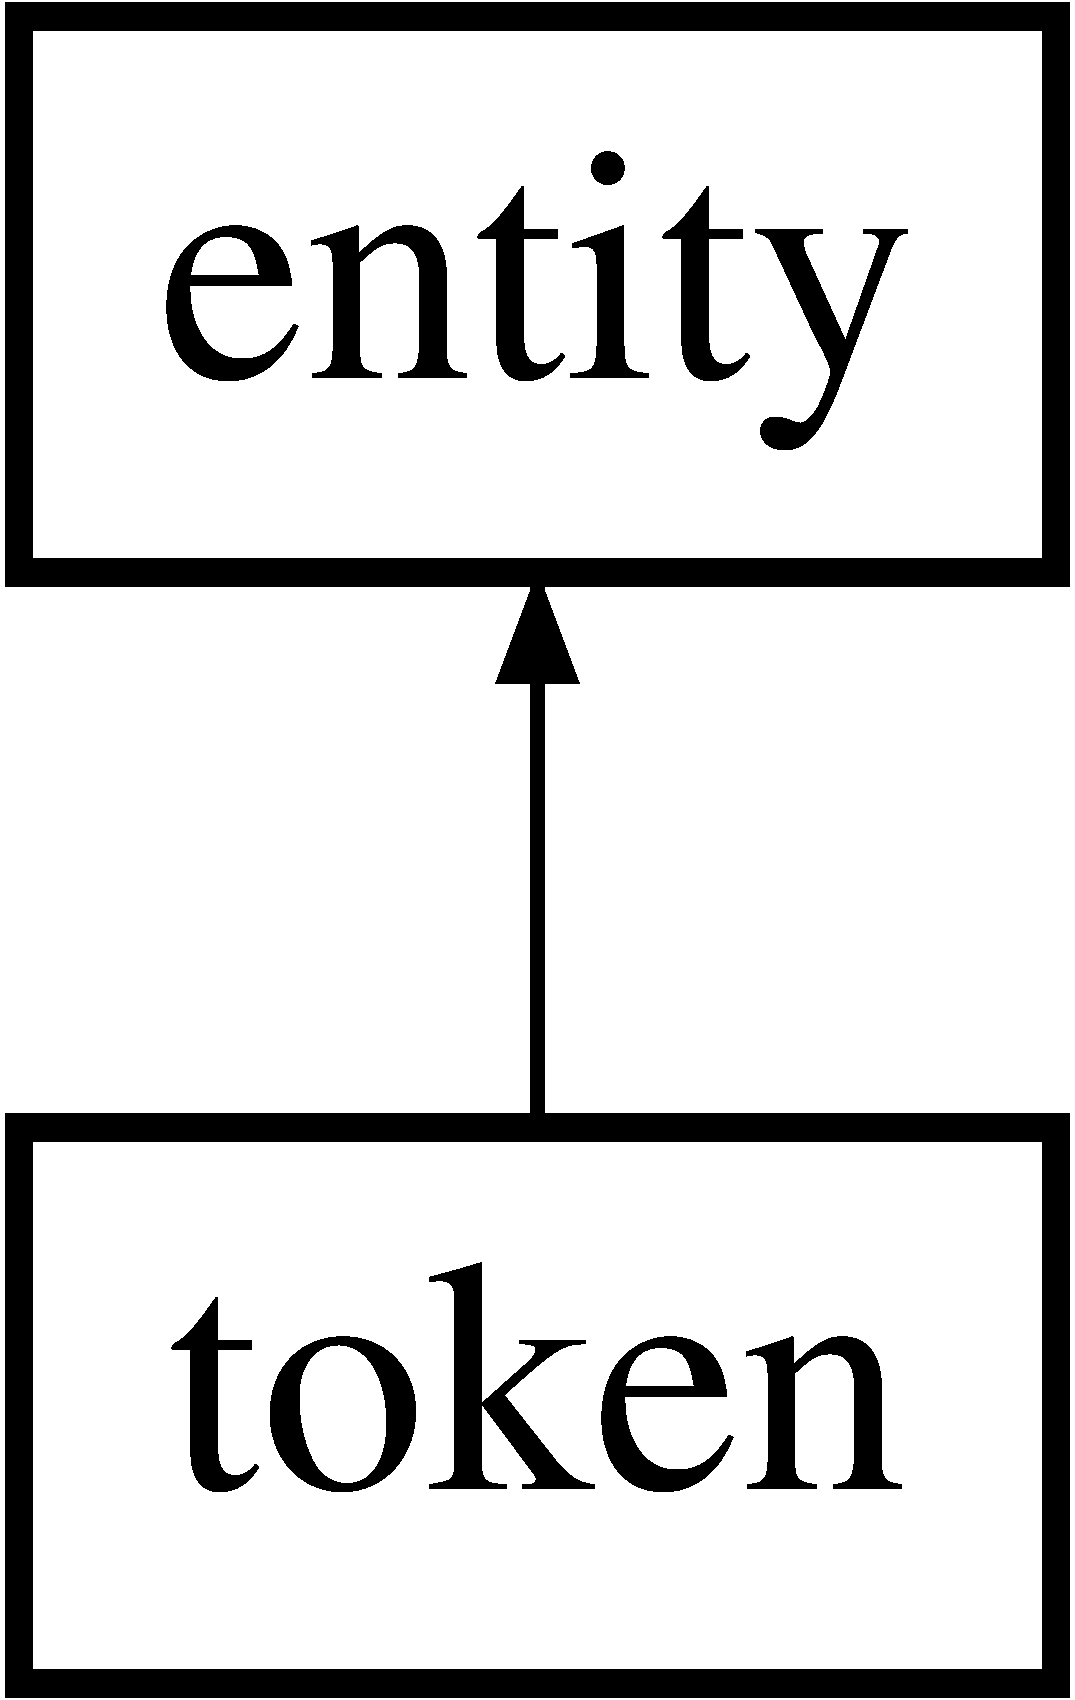
\includegraphics[height=2.000000cm]{classtoken}
\end{center}
\end{figure}
\subsection*{Public Member Functions}
\begin{DoxyCompactItemize}
\item 
\mbox{\hyperlink{classtoken_a8eea7960745130bd80f13503b0dfd887}{token}} (float x, float y, sf\+::\+Texture $\ast$\mbox{\hyperlink{classentity_aeb2014309ee421c4185f64f8cb6f6b30}{texture}})
\item 
virtual \mbox{\hyperlink{classtoken_a25ed298607d14ac675b3b320d03054af}{$\sim$token}} ()
\item 
void \mbox{\hyperlink{classtoken_aafed3b67f7f8466510d6bd4e93413e15}{update}} (const float \&dt)
\end{DoxyCompactItemize}
\subsection*{Public Attributes}
\begin{DoxyCompactItemize}
\item 
int \mbox{\hyperlink{classtoken_a01c800c05d4893b437fdcbbd54d126fa}{current\+Field\+ID}}
\end{DoxyCompactItemize}
\subsection*{Additional Inherited Members}


\subsection{Detailed Description}
Klasa tokena gracza. Zwi�zana z graczem. Podklasa entity, kt�ra wykorzystuj� cz�� encji zwi�zan� z tekstur�. 

Definition at line 4 of file token.\+h.



\subsection{Constructor \& Destructor Documentation}
\mbox{\Hypertarget{classtoken_a8eea7960745130bd80f13503b0dfd887}\label{classtoken_a8eea7960745130bd80f13503b0dfd887}} 
\index{token@{token}!token@{token}}
\index{token@{token}!token@{token}}
\subsubsection{\texorpdfstring{token()}{token()}}
{\footnotesize\ttfamily token\+::token (\begin{DoxyParamCaption}\item[{float}]{x,  }\item[{float}]{y,  }\item[{sf\+::\+Texture $\ast$}]{texture }\end{DoxyParamCaption})}

~\newline
Tworzy token w danym miejscu z dan� tekstur�.

Definition at line 19 of file token.\+cpp.

\mbox{\Hypertarget{classtoken_a25ed298607d14ac675b3b320d03054af}\label{classtoken_a25ed298607d14ac675b3b320d03054af}} 
\index{token@{token}!````~token@{$\sim$token}}
\index{````~token@{$\sim$token}!token@{token}}
\subsubsection{\texorpdfstring{$\sim$token()}{~token()}}
{\footnotesize\ttfamily token\+::$\sim$token (\begin{DoxyParamCaption}{ }\end{DoxyParamCaption})\hspace{0.3cm}{\ttfamily [virtual]}}



Definition at line 30 of file token.\+cpp.



\subsection{Member Function Documentation}
\mbox{\Hypertarget{classtoken_aafed3b67f7f8466510d6bd4e93413e15}\label{classtoken_aafed3b67f7f8466510d6bd4e93413e15}} 
\index{token@{token}!update@{update}}
\index{update@{update}!token@{token}}
\subsubsection{\texorpdfstring{update()}{update()}}
{\footnotesize\ttfamily void token\+::update (\begin{DoxyParamCaption}\item[{const float \&}]{dt }\end{DoxyParamCaption})\hspace{0.3cm}{\ttfamily [virtual]}}



Reimplemented from \mbox{\hyperlink{classentity_a155484fa64039b2e359cc2a99a6f09f5}{entity}}.



Definition at line 36 of file token.\+cpp.



\subsection{Member Data Documentation}
\mbox{\Hypertarget{classtoken_a01c800c05d4893b437fdcbbd54d126fa}\label{classtoken_a01c800c05d4893b437fdcbbd54d126fa}} 
\index{token@{token}!current\+Field\+ID@{current\+Field\+ID}}
\index{current\+Field\+ID@{current\+Field\+ID}!token@{token}}
\subsubsection{\texorpdfstring{current\+Field\+ID}{currentFieldID}}
{\footnotesize\ttfamily int token\+::current\+Field\+ID}



Definition at line 23 of file token.\+h.



The documentation for this class was generated from the following files\+:\begin{DoxyCompactItemize}
\item 
\mbox{\hyperlink{token_8h}{token.\+h}}\item 
\mbox{\hyperlink{token_8cpp}{token.\+cpp}}\end{DoxyCompactItemize}

\hypertarget{classtrap_field}{}\section{trap\+Field Class Reference}
\label{classtrap_field}\index{trap\+Field@{trap\+Field}}


{\ttfamily \#include $<$trap\+Field.\+h$>$}

Inheritance diagram for trap\+Field\+:\begin{figure}[H]
\begin{center}
\leavevmode
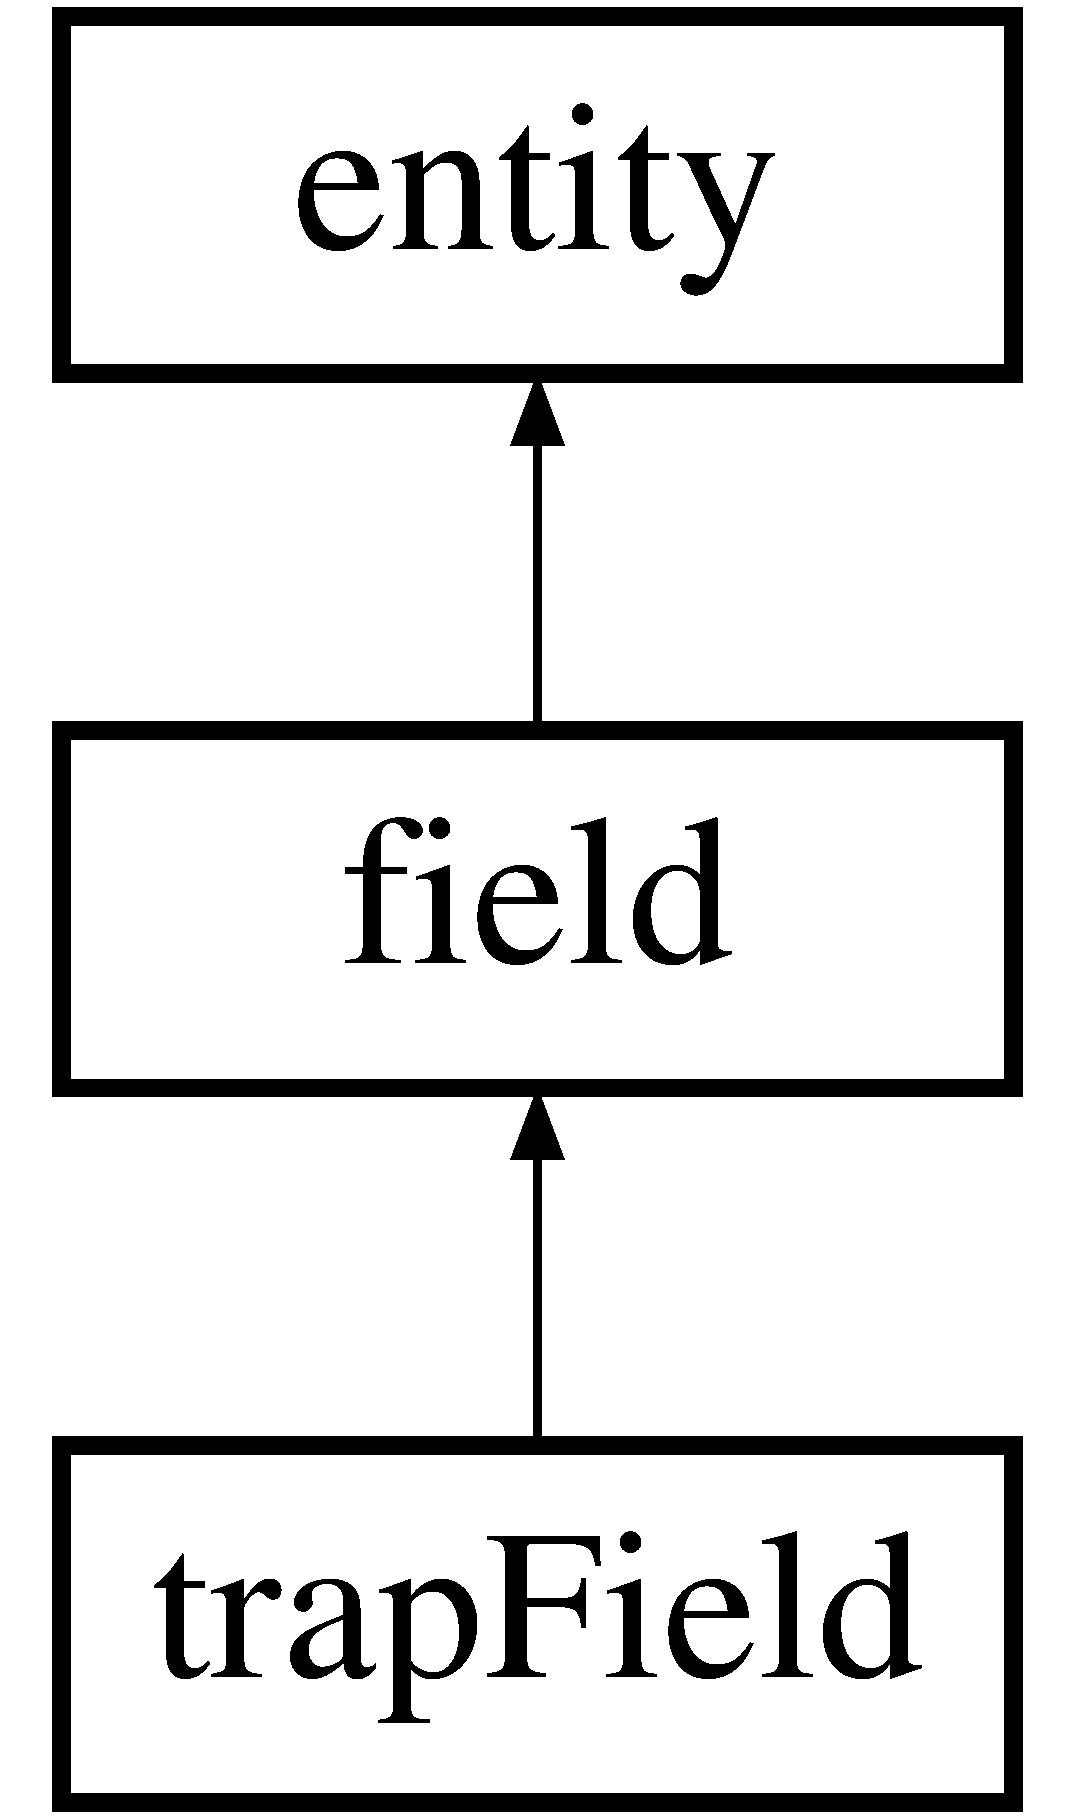
\includegraphics[height=3.000000cm]{classtrap_field}
\end{center}
\end{figure}
\subsection*{Public Member Functions}
\begin{DoxyCompactItemize}
\item 
\mbox{\hyperlink{classtrap_field_ad2320bb6dcd236ab6df3689d2c2a274e}{trap\+Field}} (std\+::string \mbox{\hyperlink{classfield_a0fa76e9bb3e439757ad10e5f6032e1ff}{field\+Title}}, std\+::string \mbox{\hyperlink{classfield_aa1ee6124b7b2c31a8cf5b72b2a1e378e}{field\+Description}}, float x, float y, float width, float height, int rotation, sf\+::\+Color \mbox{\hyperlink{classfield_ae869b5c6466855de5bb00a0da4a738e4}{color}}, float tax)
\item 
virtual \mbox{\hyperlink{classtrap_field_a97838113b62daf8e66cce2322e343814}{$\sim$trap\+Field}} ()
\item 
void \mbox{\hyperlink{classtrap_field_ad62f38751ec76b88bf7cde74ee191638}{on\+Step\+Action}} (\mbox{\hyperlink{classplayer}{player}} $\ast$\mbox{\hyperlink{classfield_a52e61f57f292aadd141aecf8745b4605}{player\+On\+Field}})
\end{DoxyCompactItemize}
\subsection*{Additional Inherited Members}


\subsection{Detailed Description}
Pole pu�apka. Pobiera pieni�dze od gracza po wst�pieniu na nie. Atrybut tax okre�la wielko�� kary pieni�nej. 

Definition at line 3 of file trap\+Field.\+h.



\subsection{Constructor \& Destructor Documentation}
\mbox{\Hypertarget{classtrap_field_ad2320bb6dcd236ab6df3689d2c2a274e}\label{classtrap_field_ad2320bb6dcd236ab6df3689d2c2a274e}} 
\index{trap\+Field@{trap\+Field}!trap\+Field@{trap\+Field}}
\index{trap\+Field@{trap\+Field}!trap\+Field@{trap\+Field}}
\subsubsection{\texorpdfstring{trap\+Field()}{trapField()}}
{\footnotesize\ttfamily trap\+Field\+::trap\+Field (\begin{DoxyParamCaption}\item[{std\+::string}]{field\+Title,  }\item[{std\+::string}]{field\+Description,  }\item[{float}]{x,  }\item[{float}]{y,  }\item[{float}]{width,  }\item[{float}]{height,  }\item[{int}]{rotation,  }\item[{sf\+::\+Color}]{color,  }\item[{float}]{tax }\end{DoxyParamCaption})}



Definition at line 4 of file trap\+Field.\+cpp.

\mbox{\Hypertarget{classtrap_field_a97838113b62daf8e66cce2322e343814}\label{classtrap_field_a97838113b62daf8e66cce2322e343814}} 
\index{trap\+Field@{trap\+Field}!````~trap\+Field@{$\sim$trap\+Field}}
\index{````~trap\+Field@{$\sim$trap\+Field}!trap\+Field@{trap\+Field}}
\subsubsection{\texorpdfstring{$\sim$trap\+Field()}{~trapField()}}
{\footnotesize\ttfamily trap\+Field\+::$\sim$trap\+Field (\begin{DoxyParamCaption}{ }\end{DoxyParamCaption})\hspace{0.3cm}{\ttfamily [virtual]}}



Definition at line 50 of file trap\+Field.\+cpp.



\subsection{Member Function Documentation}
\mbox{\Hypertarget{classtrap_field_ad62f38751ec76b88bf7cde74ee191638}\label{classtrap_field_ad62f38751ec76b88bf7cde74ee191638}} 
\index{trap\+Field@{trap\+Field}!on\+Step\+Action@{on\+Step\+Action}}
\index{on\+Step\+Action@{on\+Step\+Action}!trap\+Field@{trap\+Field}}
\subsubsection{\texorpdfstring{on\+Step\+Action()}{onStepAction()}}
{\footnotesize\ttfamily void trap\+Field\+::on\+Step\+Action (\begin{DoxyParamCaption}\item[{\mbox{\hyperlink{classplayer}{player}} $\ast$}]{player\+On\+Field }\end{DoxyParamCaption})\hspace{0.3cm}{\ttfamily [virtual]}}

~\newline
Pobiera od gracza pieni�dze za wej�cie na pole.

Implements \mbox{\hyperlink{classfield_a940f9ab5e5a33ce71f77c88c5b312300}{field}}.



Definition at line 55 of file trap\+Field.\+cpp.



The documentation for this class was generated from the following files\+:\begin{DoxyCompactItemize}
\item 
\mbox{\hyperlink{trap_field_8h}{trap\+Field.\+h}}\item 
\mbox{\hyperlink{trap_field_8cpp}{trap\+Field.\+cpp}}\end{DoxyCompactItemize}

\hypertarget{classturn}{}\section{turn Class Reference}
\label{classturn}\index{turn@{turn}}


{\ttfamily \#include $<$turn.\+h$>$}

Inheritance diagram for turn\+:\begin{figure}[H]
\begin{center}
\leavevmode
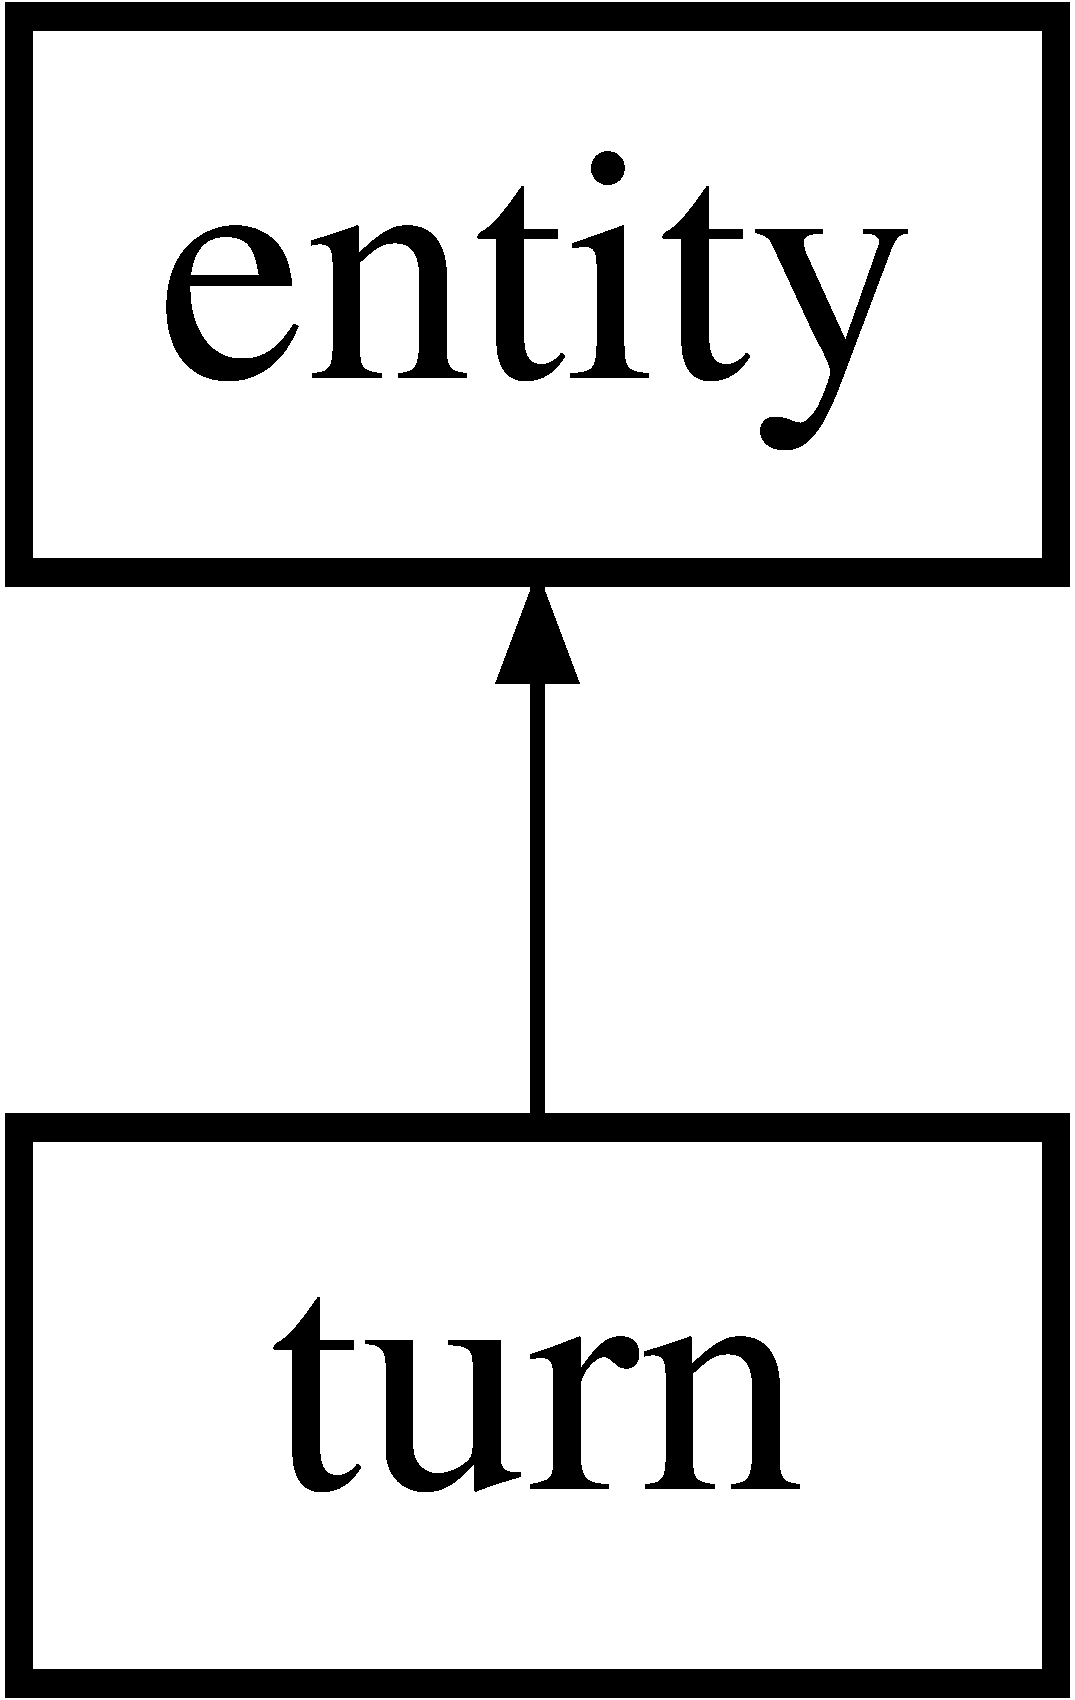
\includegraphics[height=2.000000cm]{classturn}
\end{center}
\end{figure}
\subsection*{Public Member Functions}
\begin{DoxyCompactItemize}
\item 
\mbox{\hyperlink{classturn_a6828c9caa97f36f8a4af8561511284f6}{turn}} (float x, float y, std\+::vector$<$ \mbox{\hyperlink{classplayer}{player}} $\ast$$>$ $\ast$players, std\+::vector$<$ \mbox{\hyperlink{classfield}{field}} $\ast$$>$ $\ast$fields)
\item 
virtual \mbox{\hyperlink{classturn_a9efd1e1ee9071b8a801efbb38f45dee1}{$\sim$turn}} ()
\item 
void \mbox{\hyperlink{classturn_a1753fbede73daa717c037e47eb8c86a1}{pass\+Turn}} ()
\item 
void \mbox{\hyperlink{classturn_a0e4da0dd97f0b1f5b81f786538b53cd6}{set\+Queue}} ()
\item 
void \mbox{\hyperlink{classturn_a4c1afc2c2e7711a100c5aa4c06babf2a}{update\+Your\+Turn}} (const float \&dt, sf\+::\+Vector2f mouse\+Pos)
\item 
void \mbox{\hyperlink{classturn_aa0947dcb165c2dc20131dcab556b9136}{wait\+For\+Turn}} ()
\item 
void \mbox{\hyperlink{classturn_a7ca9363b736aec69027316d35984ccde}{update\+Buttons}} (sf\+::\+Vector2f mouse\+Pos\+View, const float \&dt)
\item 
void \mbox{\hyperlink{classturn_a3fb807ea6aa45cdda7c93bb5d94435b1}{render\+Buttons}} (sf\+::\+Render\+Target $\ast$target)
\item 
void \mbox{\hyperlink{classturn_ae1c77b917de5baeb6a4df1be43e9c257}{render\+Turn\+Info}} (sf\+::\+Render\+Target $\ast$target)
\item 
void \mbox{\hyperlink{classturn_a9c139ad9e0b8455e247f0ba7b6506654}{update\+Turn\+Info}} (const float \&dt)
\item 
void \mbox{\hyperlink{classturn_a777f9c9ed46cec5eda6032dd47142c35}{render\+Dice}} (sf\+::\+Render\+Target $\ast$target)
\item 
void \mbox{\hyperlink{classturn_a3ba6c59bc823bc2cd548e49bcae7bee7}{update\+Dice}} ()
\item 
void \mbox{\hyperlink{classturn_a8c4f08e2aaf3cec484c54a96b41f307f}{move\+Token\+To\+ID}} (\mbox{\hyperlink{classtoken}{token}} $\ast$token\+To\+Move, int field\+ID)
\item 
void \mbox{\hyperlink{classturn_ad94df8997629f72e4531566d285fa58a}{move\+Token}} (\mbox{\hyperlink{classtoken}{token}} $\ast$token\+To\+Move, int num\+Of\+Fields)
\item 
void \mbox{\hyperlink{classturn_a6a72d11a8e3d8272c6b8d1ddd66331c2}{render}} (sf\+::\+Render\+Target $\ast$target)
\item 
void \mbox{\hyperlink{classturn_aff6376729f656664d68c0917e37c41f3}{update}} (const float \&dt, sf\+::\+Vector2f mouse\+Pos)
\end{DoxyCompactItemize}
\subsection*{Public Attributes}
\begin{DoxyCompactItemize}
\item 
\mbox{\hyperlink{classplayer}{player}} $\ast$ \mbox{\hyperlink{classturn_a93c4057955c746212bf09ebfdcb4eeab}{you}}
\end{DoxyCompactItemize}
\subsection*{Additional Inherited Members}


\subsection{Detailed Description}
klasa tury. Zawiera list� graczy oraz kolejk�, a tak�e wska�nik na gracza na jego komputerze. Zawiera najwa�niejsz� cz�� logiki. 

Definition at line 8 of file turn.\+h.



\subsection{Constructor \& Destructor Documentation}
\mbox{\Hypertarget{classturn_a6828c9caa97f36f8a4af8561511284f6}\label{classturn_a6828c9caa97f36f8a4af8561511284f6}} 
\index{turn@{turn}!turn@{turn}}
\index{turn@{turn}!turn@{turn}}
\subsubsection{\texorpdfstring{turn()}{turn()}}
{\footnotesize\ttfamily turn\+::turn (\begin{DoxyParamCaption}\item[{float}]{x,  }\item[{float}]{y,  }\item[{std\+::vector$<$ \mbox{\hyperlink{classplayer}{player}} $\ast$$>$ $\ast$}]{players,  }\item[{std\+::vector$<$ \mbox{\hyperlink{classfield}{field}} $\ast$$>$ $\ast$}]{fields }\end{DoxyParamCaption})}



Definition at line 3 of file turn.\+cpp.

\mbox{\Hypertarget{classturn_a9efd1e1ee9071b8a801efbb38f45dee1}\label{classturn_a9efd1e1ee9071b8a801efbb38f45dee1}} 
\index{turn@{turn}!````~turn@{$\sim$turn}}
\index{````~turn@{$\sim$turn}!turn@{turn}}
\subsubsection{\texorpdfstring{$\sim$turn()}{~turn()}}
{\footnotesize\ttfamily turn\+::$\sim$turn (\begin{DoxyParamCaption}{ }\end{DoxyParamCaption})\hspace{0.3cm}{\ttfamily [virtual]}}



Definition at line 18 of file turn.\+cpp.



\subsection{Member Function Documentation}
\mbox{\Hypertarget{classturn_ad94df8997629f72e4531566d285fa58a}\label{classturn_ad94df8997629f72e4531566d285fa58a}} 
\index{turn@{turn}!move\+Token@{move\+Token}}
\index{move\+Token@{move\+Token}!turn@{turn}}
\subsubsection{\texorpdfstring{move\+Token()}{moveToken()}}
{\footnotesize\ttfamily void turn\+::move\+Token (\begin{DoxyParamCaption}\item[{\mbox{\hyperlink{classtoken}{token}} $\ast$}]{token\+To\+Move,  }\item[{int}]{num\+Of\+Fields }\end{DoxyParamCaption})}

~\newline
Przesuwa token o okre�lon� liczb� p�l.

Definition at line 261 of file turn.\+cpp.

\mbox{\Hypertarget{classturn_a8c4f08e2aaf3cec484c54a96b41f307f}\label{classturn_a8c4f08e2aaf3cec484c54a96b41f307f}} 
\index{turn@{turn}!move\+Token\+To\+ID@{move\+Token\+To\+ID}}
\index{move\+Token\+To\+ID@{move\+Token\+To\+ID}!turn@{turn}}
\subsubsection{\texorpdfstring{move\+Token\+To\+I\+D()}{moveTokenToID()}}
{\footnotesize\ttfamily void turn\+::move\+Token\+To\+ID (\begin{DoxyParamCaption}\item[{\mbox{\hyperlink{classtoken}{token}} $\ast$}]{token\+To\+Move,  }\item[{int}]{field\+ID }\end{DoxyParamCaption})}

~\newline
Przesuwa token do pola o zadanym ID.

Definition at line 247 of file turn.\+cpp.

\mbox{\Hypertarget{classturn_a1753fbede73daa717c037e47eb8c86a1}\label{classturn_a1753fbede73daa717c037e47eb8c86a1}} 
\index{turn@{turn}!pass\+Turn@{pass\+Turn}}
\index{pass\+Turn@{pass\+Turn}!turn@{turn}}
\subsubsection{\texorpdfstring{pass\+Turn()}{passTurn()}}
{\footnotesize\ttfamily void turn\+::pass\+Turn (\begin{DoxyParamCaption}{ }\end{DoxyParamCaption})}

~\newline
Przekazuje tur� do nastepnego gracza w kolejce.

Definition at line 31 of file turn.\+cpp.

\mbox{\Hypertarget{classturn_a6a72d11a8e3d8272c6b8d1ddd66331c2}\label{classturn_a6a72d11a8e3d8272c6b8d1ddd66331c2}} 
\index{turn@{turn}!render@{render}}
\index{render@{render}!turn@{turn}}
\subsubsection{\texorpdfstring{render()}{render()}}
{\footnotesize\ttfamily void turn\+::render (\begin{DoxyParamCaption}\item[{sf\+::\+Render\+Target $\ast$}]{target }\end{DoxyParamCaption})\hspace{0.3cm}{\ttfamily [virtual]}}



Reimplemented from \mbox{\hyperlink{classentity_a5b083ead5c77ab929809c662d71f37f6}{entity}}.



Definition at line 98 of file turn.\+cpp.

\mbox{\Hypertarget{classturn_a3fb807ea6aa45cdda7c93bb5d94435b1}\label{classturn_a3fb807ea6aa45cdda7c93bb5d94435b1}} 
\index{turn@{turn}!render\+Buttons@{render\+Buttons}}
\index{render\+Buttons@{render\+Buttons}!turn@{turn}}
\subsubsection{\texorpdfstring{render\+Buttons()}{renderButtons()}}
{\footnotesize\ttfamily void turn\+::render\+Buttons (\begin{DoxyParamCaption}\item[{sf\+::\+Render\+Target $\ast$}]{target }\end{DoxyParamCaption})}



Definition at line 201 of file turn.\+cpp.

\mbox{\Hypertarget{classturn_a777f9c9ed46cec5eda6032dd47142c35}\label{classturn_a777f9c9ed46cec5eda6032dd47142c35}} 
\index{turn@{turn}!render\+Dice@{render\+Dice}}
\index{render\+Dice@{render\+Dice}!turn@{turn}}
\subsubsection{\texorpdfstring{render\+Dice()}{renderDice()}}
{\footnotesize\ttfamily void turn\+::render\+Dice (\begin{DoxyParamCaption}\item[{sf\+::\+Render\+Target $\ast$}]{target }\end{DoxyParamCaption})}



Definition at line 226 of file turn.\+cpp.

\mbox{\Hypertarget{classturn_ae1c77b917de5baeb6a4df1be43e9c257}\label{classturn_ae1c77b917de5baeb6a4df1be43e9c257}} 
\index{turn@{turn}!render\+Turn\+Info@{render\+Turn\+Info}}
\index{render\+Turn\+Info@{render\+Turn\+Info}!turn@{turn}}
\subsubsection{\texorpdfstring{render\+Turn\+Info()}{renderTurnInfo()}}
{\footnotesize\ttfamily void turn\+::render\+Turn\+Info (\begin{DoxyParamCaption}\item[{sf\+::\+Render\+Target $\ast$}]{target }\end{DoxyParamCaption})}



Definition at line 213 of file turn.\+cpp.

\mbox{\Hypertarget{classturn_a0e4da0dd97f0b1f5b81f786538b53cd6}\label{classturn_a0e4da0dd97f0b1f5b81f786538b53cd6}} 
\index{turn@{turn}!set\+Queue@{set\+Queue}}
\index{set\+Queue@{set\+Queue}!turn@{turn}}
\subsubsection{\texorpdfstring{set\+Queue()}{setQueue()}}
{\footnotesize\ttfamily void turn\+::set\+Queue (\begin{DoxyParamCaption}{ }\end{DoxyParamCaption})}

~\newline
Ustala kolejk� graczy.

Definition at line 45 of file turn.\+cpp.

\mbox{\Hypertarget{classturn_aff6376729f656664d68c0917e37c41f3}\label{classturn_aff6376729f656664d68c0917e37c41f3}} 
\index{turn@{turn}!update@{update}}
\index{update@{update}!turn@{turn}}
\subsubsection{\texorpdfstring{update()}{update()}}
{\footnotesize\ttfamily void turn\+::update (\begin{DoxyParamCaption}\item[{const float \&}]{dt,  }\item[{sf\+::\+Vector2f}]{mouse\+Pos }\end{DoxyParamCaption})}



Definition at line 114 of file turn.\+cpp.

\mbox{\Hypertarget{classturn_a7ca9363b736aec69027316d35984ccde}\label{classturn_a7ca9363b736aec69027316d35984ccde}} 
\index{turn@{turn}!update\+Buttons@{update\+Buttons}}
\index{update\+Buttons@{update\+Buttons}!turn@{turn}}
\subsubsection{\texorpdfstring{update\+Buttons()}{updateButtons()}}
{\footnotesize\ttfamily void turn\+::update\+Buttons (\begin{DoxyParamCaption}\item[{sf\+::\+Vector2f}]{mouse\+Pos\+View,  }\item[{const float \&}]{dt }\end{DoxyParamCaption})}



Definition at line 164 of file turn.\+cpp.

\mbox{\Hypertarget{classturn_a3ba6c59bc823bc2cd548e49bcae7bee7}\label{classturn_a3ba6c59bc823bc2cd548e49bcae7bee7}} 
\index{turn@{turn}!update\+Dice@{update\+Dice}}
\index{update\+Dice@{update\+Dice}!turn@{turn}}
\subsubsection{\texorpdfstring{update\+Dice()}{updateDice()}}
{\footnotesize\ttfamily void turn\+::update\+Dice (\begin{DoxyParamCaption}{ }\end{DoxyParamCaption})}

~\newline
Aktualizuje kostk� poprzez losowanie cyfry od 1 do 6.

Definition at line 235 of file turn.\+cpp.

\mbox{\Hypertarget{classturn_a9c139ad9e0b8455e247f0ba7b6506654}\label{classturn_a9c139ad9e0b8455e247f0ba7b6506654}} 
\index{turn@{turn}!update\+Turn\+Info@{update\+Turn\+Info}}
\index{update\+Turn\+Info@{update\+Turn\+Info}!turn@{turn}}
\subsubsection{\texorpdfstring{update\+Turn\+Info()}{updateTurnInfo()}}
{\footnotesize\ttfamily void turn\+::update\+Turn\+Info (\begin{DoxyParamCaption}\item[{const float \&}]{dt }\end{DoxyParamCaption})}



Definition at line 219 of file turn.\+cpp.

\mbox{\Hypertarget{classturn_a4c1afc2c2e7711a100c5aa4c06babf2a}\label{classturn_a4c1afc2c2e7711a100c5aa4c06babf2a}} 
\index{turn@{turn}!update\+Your\+Turn@{update\+Your\+Turn}}
\index{update\+Your\+Turn@{update\+Your\+Turn}!turn@{turn}}
\subsubsection{\texorpdfstring{update\+Your\+Turn()}{updateYourTurn()}}
{\footnotesize\ttfamily void turn\+::update\+Your\+Turn (\begin{DoxyParamCaption}\item[{const float \&}]{dt,  }\item[{sf\+::\+Vector2f}]{mouse\+Pos }\end{DoxyParamCaption})}



Definition at line 64 of file turn.\+cpp.

\mbox{\Hypertarget{classturn_aa0947dcb165c2dc20131dcab556b9136}\label{classturn_aa0947dcb165c2dc20131dcab556b9136}} 
\index{turn@{turn}!wait\+For\+Turn@{wait\+For\+Turn}}
\index{wait\+For\+Turn@{wait\+For\+Turn}!turn@{turn}}
\subsubsection{\texorpdfstring{wait\+For\+Turn()}{waitForTurn()}}
{\footnotesize\ttfamily void turn\+::wait\+For\+Turn (\begin{DoxyParamCaption}{ }\end{DoxyParamCaption})}

~\newline
Odblokowuje przycisk R\+O\+L\+L\+\_\+\+D\+I\+CE, gdy graczy otrzymuje ruch.

Definition at line 84 of file turn.\+cpp.



\subsection{Member Data Documentation}
\mbox{\Hypertarget{classturn_a93c4057955c746212bf09ebfdcb4eeab}\label{classturn_a93c4057955c746212bf09ebfdcb4eeab}} 
\index{turn@{turn}!you@{you}}
\index{you@{you}!turn@{turn}}
\subsubsection{\texorpdfstring{you}{you}}
{\footnotesize\ttfamily \mbox{\hyperlink{classplayer}{player}}$\ast$ turn\+::you}



Definition at line 32 of file turn.\+h.



The documentation for this class was generated from the following files\+:\begin{DoxyCompactItemize}
\item 
\mbox{\hyperlink{turn_8h}{turn.\+h}}\item 
\mbox{\hyperlink{turn_8cpp}{turn.\+cpp}}\end{DoxyCompactItemize}

\chapter{File Documentation}
\hypertarget{board_8cpp}{}\section{board.\+cpp File Reference}
\label{board_8cpp}\index{board.\+cpp@{board.\+cpp}}
{\ttfamily \#include \char`\"{}board.\+h\char`\"{}}\newline

\hypertarget{board_8h}{}\section{board.\+h File Reference}
\label{board_8h}\index{board.\+h@{board.\+h}}
{\ttfamily \#include \char`\"{}turn.\+h\char`\"{}}\newline
{\ttfamily \#include \char`\"{}player.\+h\char`\"{}}\newline
\subsection*{Classes}
\begin{DoxyCompactItemize}
\item 
class \mbox{\hyperlink{classboard}{board}}
\end{DoxyCompactItemize}

\hypertarget{entity_8cpp}{}\section{entity.\+cpp File Reference}
\label{entity_8cpp}\index{entity.\+cpp@{entity.\+cpp}}
{\ttfamily \#include \char`\"{}entity.\+h\char`\"{}}\newline

\hypertarget{entity_8h}{}\section{entity.\+h File Reference}
\label{entity_8h}\index{entity.\+h@{entity.\+h}}
{\ttfamily \#include $<$vector$>$}\newline
{\ttfamily \#include $<$iostream$>$}\newline
{\ttfamily \#include $<$ctime$>$}\newline
{\ttfamily \#include $<$cstdlib$>$}\newline
{\ttfamily \#include $<$fstream$>$}\newline
{\ttfamily \#include $<$sstream$>$}\newline
{\ttfamily \#include $<$stack$>$}\newline
{\ttfamily \#include $<$map$>$}\newline
{\ttfamily \#include $<$S\+F\+M\+L/\+Graphics.\+hpp$>$}\newline
{\ttfamily \#include $<$S\+F\+M\+L/\+System.\+hpp$>$}\newline
{\ttfamily \#include $<$S\+F\+M\+L/\+Window.\+hpp$>$}\newline
{\ttfamily \#include $<$S\+F\+M\+L/\+Audio.\+hpp$>$}\newline
{\ttfamily \#include $<$S\+F\+M\+L/\+Network.\+hpp$>$}\newline
\subsection*{Classes}
\begin{DoxyCompactItemize}
\item 
class \mbox{\hyperlink{classentity}{entity}}
\end{DoxyCompactItemize}
\subsection*{Enumerations}
\begin{DoxyCompactItemize}
\item 
enum \mbox{\hyperlink{entity_8h_a61562e49f0706841395d173cc957af1b}{font\+\_\+sizes}} \{ \mbox{\hyperlink{entity_8h_a61562e49f0706841395d173cc957af1ba03a4ccd03b30c54d540453443b2ae075}{B\+I\+G\+\_\+\+F\+O\+NT}}, 
\mbox{\hyperlink{entity_8h_a61562e49f0706841395d173cc957af1bae67fd1fbe5a53a8fe2ead8b4b1bd5686}{M\+E\+D\+I\+U\+M\+\_\+\+F\+O\+NT}}, 
\mbox{\hyperlink{entity_8h_a61562e49f0706841395d173cc957af1ba76b4fac32e6480bc5841f5f308bb33d8}{S\+M\+A\+L\+L\+\_\+\+F\+O\+NT}}
 \}
\end{DoxyCompactItemize}


\subsection{Enumeration Type Documentation}
\mbox{\Hypertarget{entity_8h_a61562e49f0706841395d173cc957af1b}\label{entity_8h_a61562e49f0706841395d173cc957af1b}} 
\index{entity.\+h@{entity.\+h}!font\+\_\+sizes@{font\+\_\+sizes}}
\index{font\+\_\+sizes@{font\+\_\+sizes}!entity.\+h@{entity.\+h}}
\subsubsection{\texorpdfstring{font\+\_\+sizes}{font\_sizes}}
{\footnotesize\ttfamily enum \mbox{\hyperlink{entity_8h_a61562e49f0706841395d173cc957af1b}{font\+\_\+sizes}}}

\begin{DoxyEnumFields}{Enumerator}
\raisebox{\heightof{T}}[0pt][0pt]{\index{B\+I\+G\+\_\+\+F\+O\+NT@{B\+I\+G\+\_\+\+F\+O\+NT}!entity.\+h@{entity.\+h}}\index{entity.\+h@{entity.\+h}!B\+I\+G\+\_\+\+F\+O\+NT@{B\+I\+G\+\_\+\+F\+O\+NT}}}\mbox{\Hypertarget{entity_8h_a61562e49f0706841395d173cc957af1ba03a4ccd03b30c54d540453443b2ae075}\label{entity_8h_a61562e49f0706841395d173cc957af1ba03a4ccd03b30c54d540453443b2ae075}} 
B\+I\+G\+\_\+\+F\+O\+NT&\\
\hline

\raisebox{\heightof{T}}[0pt][0pt]{\index{M\+E\+D\+I\+U\+M\+\_\+\+F\+O\+NT@{M\+E\+D\+I\+U\+M\+\_\+\+F\+O\+NT}!entity.\+h@{entity.\+h}}\index{entity.\+h@{entity.\+h}!M\+E\+D\+I\+U\+M\+\_\+\+F\+O\+NT@{M\+E\+D\+I\+U\+M\+\_\+\+F\+O\+NT}}}\mbox{\Hypertarget{entity_8h_a61562e49f0706841395d173cc957af1bae67fd1fbe5a53a8fe2ead8b4b1bd5686}\label{entity_8h_a61562e49f0706841395d173cc957af1bae67fd1fbe5a53a8fe2ead8b4b1bd5686}} 
M\+E\+D\+I\+U\+M\+\_\+\+F\+O\+NT&\\
\hline

\raisebox{\heightof{T}}[0pt][0pt]{\index{S\+M\+A\+L\+L\+\_\+\+F\+O\+NT@{S\+M\+A\+L\+L\+\_\+\+F\+O\+NT}!entity.\+h@{entity.\+h}}\index{entity.\+h@{entity.\+h}!S\+M\+A\+L\+L\+\_\+\+F\+O\+NT@{S\+M\+A\+L\+L\+\_\+\+F\+O\+NT}}}\mbox{\Hypertarget{entity_8h_a61562e49f0706841395d173cc957af1ba76b4fac32e6480bc5841f5f308bb33d8}\label{entity_8h_a61562e49f0706841395d173cc957af1ba76b4fac32e6480bc5841f5f308bb33d8}} 
S\+M\+A\+L\+L\+\_\+\+F\+O\+NT&\\
\hline

\end{DoxyEnumFields}


Definition at line 18 of file entity.\+h.


\hypertarget{field_8cpp}{}\section{field.\+cpp File Reference}
\label{field_8cpp}\index{field.\+cpp@{field.\+cpp}}
{\ttfamily \#include \char`\"{}field.\+h\char`\"{}}\newline

\hypertarget{field_8h}{}\section{field.\+h File Reference}
\label{field_8h}\index{field.\+h@{field.\+h}}
{\ttfamily \#include \char`\"{}entity.\+h\char`\"{}}\newline
{\ttfamily \#include \char`\"{}player.\+h\char`\"{}}\newline
\subsection*{Classes}
\begin{DoxyCompactItemize}
\item 
class \mbox{\hyperlink{classfield}{field}}
\end{DoxyCompactItemize}

\hypertarget{button_8cpp}{}\section{from\+\_\+previous\+\_\+tuts/button.cpp File Reference}
\label{button_8cpp}\index{from\+\_\+previous\+\_\+tuts/button.\+cpp@{from\+\_\+previous\+\_\+tuts/button.\+cpp}}

\hypertarget{button_8h}{}\section{from\+\_\+previous\+\_\+tuts/button.h File Reference}
\label{button_8h}\index{from\+\_\+previous\+\_\+tuts/button.\+h@{from\+\_\+previous\+\_\+tuts/button.\+h}}
{\ttfamily \#include $<$iostream$>$}\newline
{\ttfamily \#include $<$S\+F\+M\+L/\+Graphics.\+hpp$>$}\newline
\subsection*{Classes}
\begin{DoxyCompactItemize}
\item 
class \mbox{\hyperlink{class_button}{Button}}
\end{DoxyCompactItemize}

\hypertarget{gui__tests_8cpp}{}\section{from\+\_\+previous\+\_\+tuts/gui\+\_\+tests.cpp File Reference}
\label{gui__tests_8cpp}\index{from\+\_\+previous\+\_\+tuts/gui\+\_\+tests.\+cpp@{from\+\_\+previous\+\_\+tuts/gui\+\_\+tests.\+cpp}}
{\ttfamily \#include $<$S\+F\+M\+L/\+Graphics.\+hpp$>$}\newline
{\ttfamily \#include \char`\"{}text\+Box.\+h\char`\"{}}\newline
{\ttfamily \#include \char`\"{}button.\+h\char`\"{}}\newline
{\ttfamily \#include $<$iostream$>$}\newline
\subsection*{Functions}
\begin{DoxyCompactItemize}
\item 
void \mbox{\hyperlink{gui__tests_8cpp_a34e47757321d88f0d5cd514f1397aada}{gui\+\_\+tests}} ()
\end{DoxyCompactItemize}


\subsection{Function Documentation}
\mbox{\Hypertarget{gui__tests_8cpp_a34e47757321d88f0d5cd514f1397aada}\label{gui__tests_8cpp_a34e47757321d88f0d5cd514f1397aada}} 
\index{gui\+\_\+tests.\+cpp@{gui\+\_\+tests.\+cpp}!gui\+\_\+tests@{gui\+\_\+tests}}
\index{gui\+\_\+tests@{gui\+\_\+tests}!gui\+\_\+tests.\+cpp@{gui\+\_\+tests.\+cpp}}
\subsubsection{\texorpdfstring{gui\+\_\+tests()}{gui\_tests()}}
{\footnotesize\ttfamily void gui\+\_\+tests (\begin{DoxyParamCaption}{ }\end{DoxyParamCaption})}



Definition at line 6 of file gui\+\_\+tests.\+cpp.


\hypertarget{text_box_8h}{}\section{from\+\_\+previous\+\_\+tuts/text\+Box.h File Reference}
\label{text_box_8h}\index{from\+\_\+previous\+\_\+tuts/text\+Box.\+h@{from\+\_\+previous\+\_\+tuts/text\+Box.\+h}}
{\ttfamily \#include $<$iostream$>$}\newline
{\ttfamily \#include $<$sstream$>$}\newline
{\ttfamily \#include $<$S\+F\+M\+L/\+Graphics.\+hpp$>$}\newline
\subsection*{Classes}
\begin{DoxyCompactItemize}
\item 
class \mbox{\hyperlink{classtext_box}{text\+Box}}
\end{DoxyCompactItemize}
\subsection*{Macros}
\begin{DoxyCompactItemize}
\item 
\#define \mbox{\hyperlink{text_box_8h_a5a6b2a4537cccad5a1b8568904a5ee1e}{D\+E\+L\+E\+T\+E\+\_\+\+K\+EY}}~8
\item 
\#define \mbox{\hyperlink{text_box_8h_afba17fd121bcd7abc852f1ae1f3abb58}{E\+N\+T\+E\+R\+\_\+\+K\+EY}}~13
\item 
\#define \mbox{\hyperlink{text_box_8h_a4c2609b38a3373c688d3888fd50808a6}{E\+S\+C\+A\+P\+E\+\_\+\+K\+EY}}~27
\end{DoxyCompactItemize}


\subsection{Macro Definition Documentation}
\mbox{\Hypertarget{text_box_8h_a5a6b2a4537cccad5a1b8568904a5ee1e}\label{text_box_8h_a5a6b2a4537cccad5a1b8568904a5ee1e}} 
\index{text\+Box.\+h@{text\+Box.\+h}!D\+E\+L\+E\+T\+E\+\_\+\+K\+EY@{D\+E\+L\+E\+T\+E\+\_\+\+K\+EY}}
\index{D\+E\+L\+E\+T\+E\+\_\+\+K\+EY@{D\+E\+L\+E\+T\+E\+\_\+\+K\+EY}!text\+Box.\+h@{text\+Box.\+h}}
\subsubsection{\texorpdfstring{D\+E\+L\+E\+T\+E\+\_\+\+K\+EY}{DELETE\_KEY}}
{\footnotesize\ttfamily \#define D\+E\+L\+E\+T\+E\+\_\+\+K\+EY~8}



Definition at line 8 of file text\+Box.\+h.

\mbox{\Hypertarget{text_box_8h_afba17fd121bcd7abc852f1ae1f3abb58}\label{text_box_8h_afba17fd121bcd7abc852f1ae1f3abb58}} 
\index{text\+Box.\+h@{text\+Box.\+h}!E\+N\+T\+E\+R\+\_\+\+K\+EY@{E\+N\+T\+E\+R\+\_\+\+K\+EY}}
\index{E\+N\+T\+E\+R\+\_\+\+K\+EY@{E\+N\+T\+E\+R\+\_\+\+K\+EY}!text\+Box.\+h@{text\+Box.\+h}}
\subsubsection{\texorpdfstring{E\+N\+T\+E\+R\+\_\+\+K\+EY}{ENTER\_KEY}}
{\footnotesize\ttfamily \#define E\+N\+T\+E\+R\+\_\+\+K\+EY~13}



Definition at line 9 of file text\+Box.\+h.

\mbox{\Hypertarget{text_box_8h_a4c2609b38a3373c688d3888fd50808a6}\label{text_box_8h_a4c2609b38a3373c688d3888fd50808a6}} 
\index{text\+Box.\+h@{text\+Box.\+h}!E\+S\+C\+A\+P\+E\+\_\+\+K\+EY@{E\+S\+C\+A\+P\+E\+\_\+\+K\+EY}}
\index{E\+S\+C\+A\+P\+E\+\_\+\+K\+EY@{E\+S\+C\+A\+P\+E\+\_\+\+K\+EY}!text\+Box.\+h@{text\+Box.\+h}}
\subsubsection{\texorpdfstring{E\+S\+C\+A\+P\+E\+\_\+\+K\+EY}{ESCAPE\_KEY}}
{\footnotesize\ttfamily \#define E\+S\+C\+A\+P\+E\+\_\+\+K\+EY~27}



Definition at line 10 of file text\+Box.\+h.


\hypertarget{game_8cpp}{}\section{game.\+cpp File Reference}
\label{game_8cpp}\index{game.\+cpp@{game.\+cpp}}
{\ttfamily \#include \char`\"{}game.\+h\char`\"{}}\newline

\hypertarget{game_8h}{}\section{game.\+h File Reference}
\label{game_8h}\index{game.\+h@{game.\+h}}
{\ttfamily \#include \char`\"{}game\+State.\+h\char`\"{}}\newline
{\ttfamily \#include \char`\"{}main\+Menu\+State.\+h\char`\"{}}\newline
\subsection*{Classes}
\begin{DoxyCompactItemize}
\item 
class \mbox{\hyperlink{classgame}{game}}
\end{DoxyCompactItemize}

\hypertarget{game_state_8cpp}{}\section{game\+State.\+cpp File Reference}
\label{game_state_8cpp}\index{game\+State.\+cpp@{game\+State.\+cpp}}
{\ttfamily \#include \char`\"{}game\+State.\+h\char`\"{}}\newline

\hypertarget{game_state_8h}{}\section{game\+State.\+h File Reference}
\label{game_state_8h}\index{game\+State.\+h@{game\+State.\+h}}
{\ttfamily \#include \char`\"{}state.\+h\char`\"{}}\newline
{\ttfamily \#include \char`\"{}board.\+h\char`\"{}}\newline
{\ttfamily \#include \char`\"{}player.\+h\char`\"{}}\newline
\subsection*{Classes}
\begin{DoxyCompactItemize}
\item 
class \mbox{\hyperlink{classgame_state}{game\+State}}
\end{DoxyCompactItemize}

\hypertarget{gui_8cpp}{}\section{gui.\+cpp File Reference}
\label{gui_8cpp}\index{gui.\+cpp@{gui.\+cpp}}
{\ttfamily \#include \char`\"{}gui.\+h\char`\"{}}\newline

\hypertarget{gui_8h}{}\section{gui.\+h File Reference}
\label{gui_8h}\index{gui.\+h@{gui.\+h}}
{\ttfamily \#include $<$iostream$>$}\newline
{\ttfamily \#include $<$ctime$>$}\newline
{\ttfamily \#include $<$cstdlib$>$}\newline
{\ttfamily \#include $<$sstream$>$}\newline
{\ttfamily \#include $<$list$>$}\newline
{\ttfamily \#include $<$S\+F\+M\+L/\+Graphics.\+hpp$>$}\newline
{\ttfamily \#include $<$S\+F\+M\+L/\+System.\+hpp$>$}\newline
{\ttfamily \#include $<$S\+F\+M\+L/\+Window.\+hpp$>$}\newline
{\ttfamily \#include $<$S\+F\+M\+L/\+Audio.\+hpp$>$}\newline
{\ttfamily \#include $<$S\+F\+M\+L/\+Network.\+hpp$>$}\newline
\subsection*{Classes}
\begin{DoxyCompactItemize}
\item 
class \mbox{\hyperlink{classgui_1_1button}{gui\+::button}}
\item 
class \mbox{\hyperlink{classgui_1_1info_bar}{gui\+::info\+Bar}}
\item 
class \mbox{\hyperlink{classgui_1_1menu}{gui\+::menu}}
\end{DoxyCompactItemize}
\subsection*{Namespaces}
\begin{DoxyCompactItemize}
\item 
 \mbox{\hyperlink{namespacegui}{gui}}
\end{DoxyCompactItemize}
\subsection*{Enumerations}
\begin{DoxyCompactItemize}
\item 
enum \mbox{\hyperlink{gui_8h_a11a6094191da43b6b4568e7736fb89ba}{button\+\_\+states}} \{ \mbox{\hyperlink{gui_8h_a11a6094191da43b6b4568e7736fb89baab07455a5cba7480564ccdf0225f8d082}{B\+T\+N\+\_\+\+I\+D\+LE}} = 0, 
\mbox{\hyperlink{gui_8h_a11a6094191da43b6b4568e7736fb89baad6fdb8a1568b56acfc5a2870feef75aa}{B\+T\+N\+\_\+\+H\+O\+V\+ER}}, 
\mbox{\hyperlink{gui_8h_a11a6094191da43b6b4568e7736fb89baa076cb0f337f54dd9e2e24b0ac35e2914}{B\+T\+N\+\_\+\+P\+R\+E\+S\+S\+ED}}
 \}
\end{DoxyCompactItemize}


\subsection{Enumeration Type Documentation}
\mbox{\Hypertarget{gui_8h_a11a6094191da43b6b4568e7736fb89ba}\label{gui_8h_a11a6094191da43b6b4568e7736fb89ba}} 
\index{gui.\+h@{gui.\+h}!button\+\_\+states@{button\+\_\+states}}
\index{button\+\_\+states@{button\+\_\+states}!gui.\+h@{gui.\+h}}
\subsubsection{\texorpdfstring{button\+\_\+states}{button\_states}}
{\footnotesize\ttfamily enum \mbox{\hyperlink{gui_8h_a11a6094191da43b6b4568e7736fb89ba}{button\+\_\+states}}}

\begin{DoxyEnumFields}{Enumerator}
\raisebox{\heightof{T}}[0pt][0pt]{\index{B\+T\+N\+\_\+\+I\+D\+LE@{B\+T\+N\+\_\+\+I\+D\+LE}!gui.\+h@{gui.\+h}}\index{gui.\+h@{gui.\+h}!B\+T\+N\+\_\+\+I\+D\+LE@{B\+T\+N\+\_\+\+I\+D\+LE}}}\mbox{\Hypertarget{gui_8h_a11a6094191da43b6b4568e7736fb89baab07455a5cba7480564ccdf0225f8d082}\label{gui_8h_a11a6094191da43b6b4568e7736fb89baab07455a5cba7480564ccdf0225f8d082}} 
B\+T\+N\+\_\+\+I\+D\+LE&\\
\hline

\raisebox{\heightof{T}}[0pt][0pt]{\index{B\+T\+N\+\_\+\+H\+O\+V\+ER@{B\+T\+N\+\_\+\+H\+O\+V\+ER}!gui.\+h@{gui.\+h}}\index{gui.\+h@{gui.\+h}!B\+T\+N\+\_\+\+H\+O\+V\+ER@{B\+T\+N\+\_\+\+H\+O\+V\+ER}}}\mbox{\Hypertarget{gui_8h_a11a6094191da43b6b4568e7736fb89baad6fdb8a1568b56acfc5a2870feef75aa}\label{gui_8h_a11a6094191da43b6b4568e7736fb89baad6fdb8a1568b56acfc5a2870feef75aa}} 
B\+T\+N\+\_\+\+H\+O\+V\+ER&\\
\hline

\raisebox{\heightof{T}}[0pt][0pt]{\index{B\+T\+N\+\_\+\+P\+R\+E\+S\+S\+ED@{B\+T\+N\+\_\+\+P\+R\+E\+S\+S\+ED}!gui.\+h@{gui.\+h}}\index{gui.\+h@{gui.\+h}!B\+T\+N\+\_\+\+P\+R\+E\+S\+S\+ED@{B\+T\+N\+\_\+\+P\+R\+E\+S\+S\+ED}}}\mbox{\Hypertarget{gui_8h_a11a6094191da43b6b4568e7736fb89baa076cb0f337f54dd9e2e24b0ac35e2914}\label{gui_8h_a11a6094191da43b6b4568e7736fb89baa076cb0f337f54dd9e2e24b0ac35e2914}} 
B\+T\+N\+\_\+\+P\+R\+E\+S\+S\+ED&\\
\hline

\end{DoxyEnumFields}


Definition at line 15 of file gui.\+h.


\hypertarget{main_8cpp}{}\section{main.\+cpp File Reference}
\label{main_8cpp}\index{main.\+cpp@{main.\+cpp}}
{\ttfamily \#include \char`\"{}game.\+h\char`\"{}}\newline
\subsection*{Functions}
\begin{DoxyCompactItemize}
\item 
int \mbox{\hyperlink{main_8cpp_ae66f6b31b5ad750f1fe042a706a4e3d4}{main}} ()
\end{DoxyCompactItemize}


\subsection{Function Documentation}
\mbox{\Hypertarget{main_8cpp_ae66f6b31b5ad750f1fe042a706a4e3d4}\label{main_8cpp_ae66f6b31b5ad750f1fe042a706a4e3d4}} 
\index{main.\+cpp@{main.\+cpp}!main@{main}}
\index{main@{main}!main.\+cpp@{main.\+cpp}}
\subsubsection{\texorpdfstring{main()}{main()}}
{\footnotesize\ttfamily int main (\begin{DoxyParamCaption}{ }\end{DoxyParamCaption})}

Opis projektu 

Definition at line 159 of file main.\+cpp.


\hypertarget{main_menu_state_8cpp}{}\section{main\+Menu\+State.\+cpp File Reference}
\label{main_menu_state_8cpp}\index{main\+Menu\+State.\+cpp@{main\+Menu\+State.\+cpp}}
{\ttfamily \#include \char`\"{}main\+Menu\+State.\+h\char`\"{}}\newline

\hypertarget{main_menu_state_8h}{}\section{main\+Menu\+State.\+h File Reference}
\label{main_menu_state_8h}\index{main\+Menu\+State.\+h@{main\+Menu\+State.\+h}}
{\ttfamily \#include \char`\"{}state.\+h\char`\"{}}\newline
{\ttfamily \#include \char`\"{}gui.\+h\char`\"{}}\newline
{\ttfamily \#include \char`\"{}game\+State.\+h\char`\"{}}\newline
\subsection*{Classes}
\begin{DoxyCompactItemize}
\item 
class \mbox{\hyperlink{classmain_menu_state}{main\+Menu\+State}}
\end{DoxyCompactItemize}

\hypertarget{multiplayer__test_8cpp}{}\section{multiplayer\+\_\+test.\+cpp File Reference}
\label{multiplayer__test_8cpp}\index{multiplayer\+\_\+test.\+cpp@{multiplayer\+\_\+test.\+cpp}}
{\ttfamily \#include $<$S\+F\+M\+L/\+Network.\+hpp$>$}\newline
{\ttfamily \#include $<$S\+F\+M\+L/\+Graphics.\+hpp$>$}\newline
{\ttfamily \#include $<$iostream$>$}\newline
\subsection*{Macros}
\begin{DoxyCompactItemize}
\item 
\#define \mbox{\hyperlink{multiplayer__test_8cpp_a62ecd70800687eb2d625af180c4210d7}{T\+I\+L\+E\+\_\+\+S\+I\+ZE}}~49.f
\end{DoxyCompactItemize}
\subsection*{Functions}
\begin{DoxyCompactItemize}
\item 
int \mbox{\hyperlink{multiplayer__test_8cpp_a0e57c6a59427c491d963de4d7e65067d}{multiplayer\+\_\+test}} ()
\end{DoxyCompactItemize}


\subsection{Macro Definition Documentation}
\mbox{\Hypertarget{multiplayer__test_8cpp_a62ecd70800687eb2d625af180c4210d7}\label{multiplayer__test_8cpp_a62ecd70800687eb2d625af180c4210d7}} 
\index{multiplayer\+\_\+test.\+cpp@{multiplayer\+\_\+test.\+cpp}!T\+I\+L\+E\+\_\+\+S\+I\+ZE@{T\+I\+L\+E\+\_\+\+S\+I\+ZE}}
\index{T\+I\+L\+E\+\_\+\+S\+I\+ZE@{T\+I\+L\+E\+\_\+\+S\+I\+ZE}!multiplayer\+\_\+test.\+cpp@{multiplayer\+\_\+test.\+cpp}}
\subsubsection{\texorpdfstring{T\+I\+L\+E\+\_\+\+S\+I\+ZE}{TILE\_SIZE}}
{\footnotesize\ttfamily \#define T\+I\+L\+E\+\_\+\+S\+I\+ZE~49.f}



Definition at line 5 of file multiplayer\+\_\+test.\+cpp.



\subsection{Function Documentation}
\mbox{\Hypertarget{multiplayer__test_8cpp_a0e57c6a59427c491d963de4d7e65067d}\label{multiplayer__test_8cpp_a0e57c6a59427c491d963de4d7e65067d}} 
\index{multiplayer\+\_\+test.\+cpp@{multiplayer\+\_\+test.\+cpp}!multiplayer\+\_\+test@{multiplayer\+\_\+test}}
\index{multiplayer\+\_\+test@{multiplayer\+\_\+test}!multiplayer\+\_\+test.\+cpp@{multiplayer\+\_\+test.\+cpp}}
\subsubsection{\texorpdfstring{multiplayer\+\_\+test()}{multiplayer\_test()}}
{\footnotesize\ttfamily int multiplayer\+\_\+test (\begin{DoxyParamCaption}{ }\end{DoxyParamCaption})}



Definition at line 10 of file multiplayer\+\_\+test.\+cpp.


\hypertarget{player_8cpp}{}\section{player.\+cpp File Reference}
\label{player_8cpp}\index{player.\+cpp@{player.\+cpp}}
{\ttfamily \#include \char`\"{}player.\+h\char`\"{}}\newline

\hypertarget{player_8h}{}\section{player.\+h File Reference}
\label{player_8h}\index{player.\+h@{player.\+h}}
{\ttfamily \#include \char`\"{}token.\+h\char`\"{}}\newline
\subsection*{Classes}
\begin{DoxyCompactItemize}
\item 
class \mbox{\hyperlink{classplayer}{player}}
\end{DoxyCompactItemize}

\hypertarget{property_field_8cpp}{}\section{property\+Field.\+cpp File Reference}
\label{property_field_8cpp}\index{property\+Field.\+cpp@{property\+Field.\+cpp}}
{\ttfamily \#include \char`\"{}property\+Field.\+h\char`\"{}}\newline

\hypertarget{property_field_8h}{}\section{property\+Field.\+h File Reference}
\label{property_field_8h}\index{property\+Field.\+h@{property\+Field.\+h}}
{\ttfamily \#include \char`\"{}field.\+h\char`\"{}}\newline
{\ttfamily \#include \char`\"{}gui.\+h\char`\"{}}\newline
\subsection*{Classes}
\begin{DoxyCompactItemize}
\item 
class \mbox{\hyperlink{classproperty_field}{property\+Field}}
\end{DoxyCompactItemize}

\hypertarget{state_8cpp}{}\section{state.\+cpp File Reference}
\label{state_8cpp}\index{state.\+cpp@{state.\+cpp}}
{\ttfamily \#include \char`\"{}state.\+h\char`\"{}}\newline

\hypertarget{state_8h}{}\section{state.\+h File Reference}
\label{state_8h}\index{state.\+h@{state.\+h}}
{\ttfamily \#include $<$vector$>$}\newline
{\ttfamily \#include $<$iostream$>$}\newline
{\ttfamily \#include $<$ctime$>$}\newline
{\ttfamily \#include $<$cstdlib$>$}\newline
{\ttfamily \#include $<$fstream$>$}\newline
{\ttfamily \#include $<$sstream$>$}\newline
{\ttfamily \#include $<$stack$>$}\newline
{\ttfamily \#include $<$map$>$}\newline
{\ttfamily \#include $<$S\+F\+M\+L/\+Graphics.\+hpp$>$}\newline
{\ttfamily \#include $<$S\+F\+M\+L/\+System.\+hpp$>$}\newline
{\ttfamily \#include $<$S\+F\+M\+L/\+Window.\+hpp$>$}\newline
{\ttfamily \#include $<$S\+F\+M\+L/\+Audio.\+hpp$>$}\newline
{\ttfamily \#include $<$S\+F\+M\+L/\+Network.\+hpp$>$}\newline
\subsection*{Classes}
\begin{DoxyCompactItemize}
\item 
class \mbox{\hyperlink{classstate}{state}}
\end{DoxyCompactItemize}

\hypertarget{token_8cpp}{}\section{token.\+cpp File Reference}
\label{token_8cpp}\index{token.\+cpp@{token.\+cpp}}
{\ttfamily \#include \char`\"{}token.\+h\char`\"{}}\newline

\hypertarget{token_8h}{}\section{token.\+h File Reference}
\label{token_8h}\index{token.\+h@{token.\+h}}
{\ttfamily \#include \char`\"{}entity.\+h\char`\"{}}\newline
\subsection*{Classes}
\begin{DoxyCompactItemize}
\item 
class \mbox{\hyperlink{classtoken}{token}}
\end{DoxyCompactItemize}

\hypertarget{trap_field_8cpp}{}\section{trap\+Field.\+cpp File Reference}
\label{trap_field_8cpp}\index{trap\+Field.\+cpp@{trap\+Field.\+cpp}}
{\ttfamily \#include \char`\"{}trap\+Field.\+h\char`\"{}}\newline

\hypertarget{trap_field_8h}{}\section{trap\+Field.\+h File Reference}
\label{trap_field_8h}\index{trap\+Field.\+h@{trap\+Field.\+h}}
{\ttfamily \#include \char`\"{}field.\+h\char`\"{}}\newline
\subsection*{Classes}
\begin{DoxyCompactItemize}
\item 
class \mbox{\hyperlink{classtrap_field}{trap\+Field}}
\end{DoxyCompactItemize}

\hypertarget{turn_8cpp}{}\section{turn.\+cpp File Reference}
\label{turn_8cpp}\index{turn.\+cpp@{turn.\+cpp}}
{\ttfamily \#include \char`\"{}turn.\+h\char`\"{}}\newline

\hypertarget{turn_8h}{}\section{turn.\+h File Reference}
\label{turn_8h}\index{turn.\+h@{turn.\+h}}
{\ttfamily \#include $<$list$>$}\newline
{\ttfamily \#include \char`\"{}property\+Field.\+h\char`\"{}}\newline
{\ttfamily \#include \char`\"{}trap\+Field.\+h\char`\"{}}\newline
{\ttfamily \#include \char`\"{}gui.\+h\char`\"{}}\newline
\subsection*{Classes}
\begin{DoxyCompactItemize}
\item 
class \mbox{\hyperlink{classturn}{turn}}
\end{DoxyCompactItemize}

%--- End generated contents ---

% Index
\backmatter
\newpage
\phantomsection
\clearemptydoublepage
\addcontentsline{toc}{chapter}{Index}
\printindex

\end{document}
